\documentclass{ucbthesis}
\usepackage{mathrsfs, graphicx, bm}
\usepackage{cite}
% \usepackage{floatrow}

\usepackage{amsmath,amssymb,amsfonts,hyperref,lineno,microtype,setspace,multicol,textcomp, marvosym, algorithm,algpseudocode, algorithmicx, wrapfig, mathtools}

% To-do notes
\usepackage[colorinlistoftodos,prependcaption,textsize=small]{todonotes}
\newcommand{\mytodo}[2][1=]{\todo[linecolor=yellow,backgroundcolor=yellow!25,bordercolor=yellow,#1]{#2}}


% Set graphics path
\graphicspath{ {figures/} }

\DeclareMathOperator*{\argmax}{argmax}
\DeclareMathOperator*{\argmin}{argmin}
\DeclarePairedDelimiter\abs{\lvert}{\rvert}

\makeatletter
\let\oldabs\abs
\def\abs{\@ifstar{\oldabs}{\oldabs*}}
%
\let\oldnorm\norm
\def\norm{\@ifstar{\oldnorm}{\oldnorm*}}
\makeatother

\renewcommand{\vec}{\bm}
\newcommand{\op}{\mathcal}
\newcommand{\mat}{\mathbf}

\newcommand{\object}{\vec{x}}
\newcommand{\kernel}{\vec{h}}
\newcommand{\h}{\kernel}
\newcommand{\x}{\object}
\newcommand{\image}{\vec{y}}
\newcommand{\y}{\image}
\newcommand{\noise}{{\eta}}
\newcommand{\blurmat}{\mat{B}}
\newcommand{\B}{\blurmat}
\newcommand{\crop}{\mat{W}}
\newcommand{\W}{\crop}
\newcommand{\A}{\mat{A}}
\newcommand{\I}{\mat{I}}
\newcommand{\e}{\vec{e}}
\newcommand{\D}{\mat{D}}
\newcommand{\M}{\mat{M}}
\newcommand{\F}{\mat{F}}
\renewcommand{\top}{\mathsf{H}}


\begin{document}


\bibliographystyle{osajnl}

% Declarations for Front Matter
\title{Quantitative Microscopy using Coded Illumination}
\author{Zachary Fitzgerald Phillips}
\degreesemester{Spring}
\degreeyear{2019}
\degree{Doctor of Philosophy}
\chair{Ted Van Duzer Associate Professor Laura Waller}
\othermembers{Professor Lydia Sohn \\Assistant Professor Ren Ng}
\numberofmembers{3}

\field{Applied Science and Technology}
\campus{Berkeley}

% For a masters thesis, replace the above \documentclass line with
% \documentclass[masters]{ucbthesis}
% This affects the title and approval pages, which by default calls this
% document a "dissertation", not a "thesis".

\maketitle
% Delete (or comment out) the \approvalpage line for the final version.
% \approvalpage
\copyrightpage

\begin{center}
    \textbf{Abstract}
    
    \vspace{1.2cm}
     Quantitative Optical Microscopy Using Coded Illumination
 
    \vspace{0.4cm}
    
    By
 
    \vspace{0.4cm}
    Zachary F. Phillips
    
     \vspace{0.4cm}
     Doctor of Philosophy in Applied Science and Technology
     
     \vspace{0.4cm}
     University of California, Berkeley
     
     \vspace{0.4cm}
     Ted Van Duzer Associate Professor Laura Waller, Chair
 
    \vspace{0.8cm}

    
\end{center}

Quantitative optical microscopy continues to be a powerful tool in biology and throughout the sciences. Computational microscopy blends large-scale computation with conventional image formation principles to enable a large number of imaging modalities not possible with conventional techniques, such as quantitative phase imaging, motion deblurring, and super-resolution techniques. In this work, we present several novel examples of computational microscopy using a programmable illumination source such as a LED array to introduce known images which have been distorted by a know mathematical transformation. We first introduce quantitative phase imaging using differential phase contrast, which uses multiple measurements to recover the linearized complex field of a thin, transparent sample, and demonstrate a novel single-shot variant using color-multiplexing. Second, we explore coded illumination for high-throughput imaging, and demonstrate a temporal-coding technique which enables significantly higher SNR for high-speed slide scanning and neuropathology applications. We examine the various hardware elements which limit acquisition speeds, and provide a framework for defining when our method is advantageous over existing techniques. For fluorescent imaging, we demonstrate a 10$\times$ improvement in reconstruction SNR compared to conventional high-speed imaging techniques. Next, we explore the design and fabrication of LED illumination devices, including a quasi-dome LED illuminator which enables high-angle illumination for a variety of applications. Finally, we demonstrate two examples of self-calibration techniques for computational imaging systems employing coded illumination. These include aberration recovery using differential phase contrast and source calibration for the quasi-dome LED array, using both image-based calibration and an online method based on Fourier ptychography.

\begin{frontmatter}

% Dedication
\begin{dedication}
  \null\vfil
\begin{center}
\textit{For Mandie}
\end{center}
\vfil\null

\end{dedication}

% You can delete the \clearpage lines if you don't want these to start on
% separate pages.

\tableofcontents
\clearpage
\listoffigures

\clearpage
\begin{acknowledgements}
First and foremost, I would like to thank Associate Professor Laura Waller for providing careful guidance throughout my time at Berkeley, and for putting faith and resources behind myself and fellow lab members so that we can freely explore, create, and publish in the field of computational imaging. I would also like to thank my committee, Assistant Professor Ren Ng and Professor Lydia Sohn, for many useful conversations throughout my time at UC Berkeley. The Waller Lab has been a fantastic place to learn about the field of computational imaging, and I am grateful to each of my fellow group members. I would like to specifically thank my co-authors and collaborators within the Waller lab, including Regina Eckert, Gautam Gunjala, Michael Kellman, Nick Antipa, and David Ren. Specifically, I would like to thank Michael Chen for being an excellent collaborator in both research and entrepreneurship, and my closest neighbor, Li-Hao Yeh, with whom I have enjoyed thousands of conversations during our nearly 5 years in 558 Cory Hall. I have genuinely enjoyed my many whiteboard discussions with Sarah Dean, and feel very fortunate to have worked extensively with Post-docs Lei Tian, Volker Jaedicke, Shwetadwip Chowdhury, and Emrah Bostan. I would also like to acknowledge those who took the time to proofread this dissertation through its many iterations who have not already been mentioned: Kristina Monokhova, Michael Kellman, Henry Pinkard, and Emma Alexander.

During my time at Berkeley, I found that being productive and focused during the week requires taking time to unwind during the weekend (and occasionally during the evening). I would first like to thank my girlfriend, Chelsea, for always being a steadfast adventure partner and sounding board through the many seasons of graduate school. Since my first days in Berkeley, I've enjoyed many waves with my close friend and fellow AS\&T student Brandon Wood. I also want to thank my friends Chris Lalau-Keraly, Alex Forse, Kyle Ginthner, JB Chapman, (Day-leader) Mike Chapman, Jon Morris, Alix Charles, Mike Francis, Dan Wooten, and many others for our many good times.

Attending Berkeley has been my proudest and must fulfilling accomplishment, and it would have never been possible without my Mom, Dad, and sisters Allie and Mandie, who have always been supporting through our shared challenges as well as my own. I credit my dad, together with my grandfather, for teaching me how to break down a complicated problem into a series of small problems, and the importance of tenacity. My mother taught me the importance of a sense of humor and being personable. I would also like to acknowledge all of my grandparents, especially Phil and Bertha Phillips, who continue to teach importance of family, travel, and spending time outdoors.

I also want to thank those who helped and encouraged me prior to coming to Berkeley, including Professor Amy Oldenburg, Daniel Marks, and Raghav Chhetri.

Finally, I want to thank the many undergraduate students I've worked with, including Patrick Oare, Joel Whang, Nitin Sadras, Aditya Gande, Gautam Gunjala, Sachin Deyoung, Taehyung Kim, Paroma Varma, Jared Rulison, Sudarshan Seshadri, and Kuan Chang for their generous assistance despite their many obligations.

\end{acknowledgements}

\end{frontmatter}
\pagestyle{headings}
\chapter{Introduction}\label{ch:introduction}

\section{Optical Microscopy}

The optical microscope is one of the oldest scientific instruments, and continues to be an essential tool for researchers, clinicians, and engineers across many disciplines. Microscopes are typically defined as having two or more refractive surfaces to provide magnification between the object of interest and the imaging plane, enabling the user to see things much smaller than the normal optical resolution of the human eye. Credit for the inventor of the compound microscope is generally attributed to Hans and Zacharias Jansen~\cite{van2010origins}, although the first published work on microscope design wasn't released until 1665 (Hooke and van Leeuwenhoek)~\cite{natureMilestones,hookeMicrographica}. The term "microscope" is generally used to describe optical microscopes - those which are designed for use with light within the optical band of the electro-magnetic spectrum ($390nm \leq \lambda \leq 700nm$), which is approximately the electromagnetic spectrum detectable by the human eye.

\subsection{Imaging and Resolution}
Light interacts with our world in many ways, including diffraction, refraction, reflection, and absorption. At optical wavelengths, many common materials (usually a ceramic such as glass) have favorable properties for refractive optics (providing significant phase delay with little absorption), facilitating a precise control of an optical signal using these elements. Imaging is the process of creating a copy of a particular optical signal at a different position in space, which is generally coincident with a film or electronic detector. In the simplest case, a single lens may be used to form a magnified image of an optical signal by placing the lens and detector at a particular distance from the sample - this situation is described by the imaging condition,

\begin{equation}
\frac{1}{f} = \frac{1}{s_o} + \frac{1}{s_i}
\end{equation}

\noindent which relates the distance of an optical element to a object under observation ($s_o$) to the distance of a conjugate image ($s_i$), which is be magnified by a factor $M = \frac{-s_i}{s_o}$ based on these distances and the focal length of the optical element ($f$). A single-lens imaging system imposes many practical issues, including telecentricity (consistency of magnification across the field) and aberrations, both geometric and chromatic. Including multiple optical elements into a compound microscope can dramatically improve image quality by providing aberration compensation and telecentricity. Typically, the exact number and design of these components is abstracted to the end-user and can be defined by a relatively low number of descriptive quantities despite the complex internal lens design of a modern microscope objective. Magnification and numerical aperture (NA) are the most important of these physical quantities; the magnification of an objective sets the field of view, which is relayed by the optic, while the NA sets a minimum bound on the diffraction-limited resolution. The numerical aperture is defined by the formula $NA=n\sin (\theta)$, where $n$ is the refractive index of the medium, and $\theta$ is the maximum half-angle at which light may pass through the objective relative to the radial (optical) axis. The angular dependence of numerical aperture is completely described by interference effects which arise from the wave-optics model of light propagation. As multiple off-axis sources of the same wavelength converge to a point, the wavefronts of these sources will cause constructive and destructive interference. The minimum distance between two peaks formed by constructive interference is proportional to both the wavelength of the illumination and the angular separation between the two beams (which is set by the maximum NA of the illumination source and imaging optics). Practically, the size of this spot defines the resolution of the optical system. By the Rayleigh criteria, the resolution of an optical system is defined as:

\begin{equation}\label{eq:intro:rayleigh}
\Delta x_{min}  = \frac{1.22 \lambda}{(NA_{objective} + NA_{illumination})}
\end{equation}

This quantity defines the minimum separation between two points which can be detected by a system with a circular aperture and is defined by the distance between the center if the point spread function (PSF) and it's first null. Note that Eq.~\ref{eq:intro:rayleigh} is dependent on both detection side NA ($NA_{objective}$) and illumination side NA ($NA_{illumination}$). The ratio between these NA, typically denoted as $\sigma = NA_{objective}/NA_{Illumination}$, is sometimes referred to as the coherence factor. As $\sigma \longrightarrow 0 $, the illumination becomes spatially coherent, meaning the phase of the illumination wavefront at a given point on the sample can be perfectly described by all other points on the sample. This definition assumes that the light source is composed of spatially distributed statistically uncorrelated emitters - contemporary microscope sources such as halogen and tungsten lamps satisfy this criterion while in k{\"o}hler geometry. As sigma increases, the minimum resolvable feature size decreases, leading to images of higher quality, subject to aliasing affects. However, increasing $\sigma$ beyond 1 does not provide further resolution improvement due to the ballistic light (DC term) is not collected by the objective. This is the working principle of dark-field microscopy, which reveals high-resolution features, but does not localize them beyond the resolution of the imaging optics.

\subsection{Fourier Optics Description}


\section{Computational Microscopy}

\begin{figure}
    \centering
    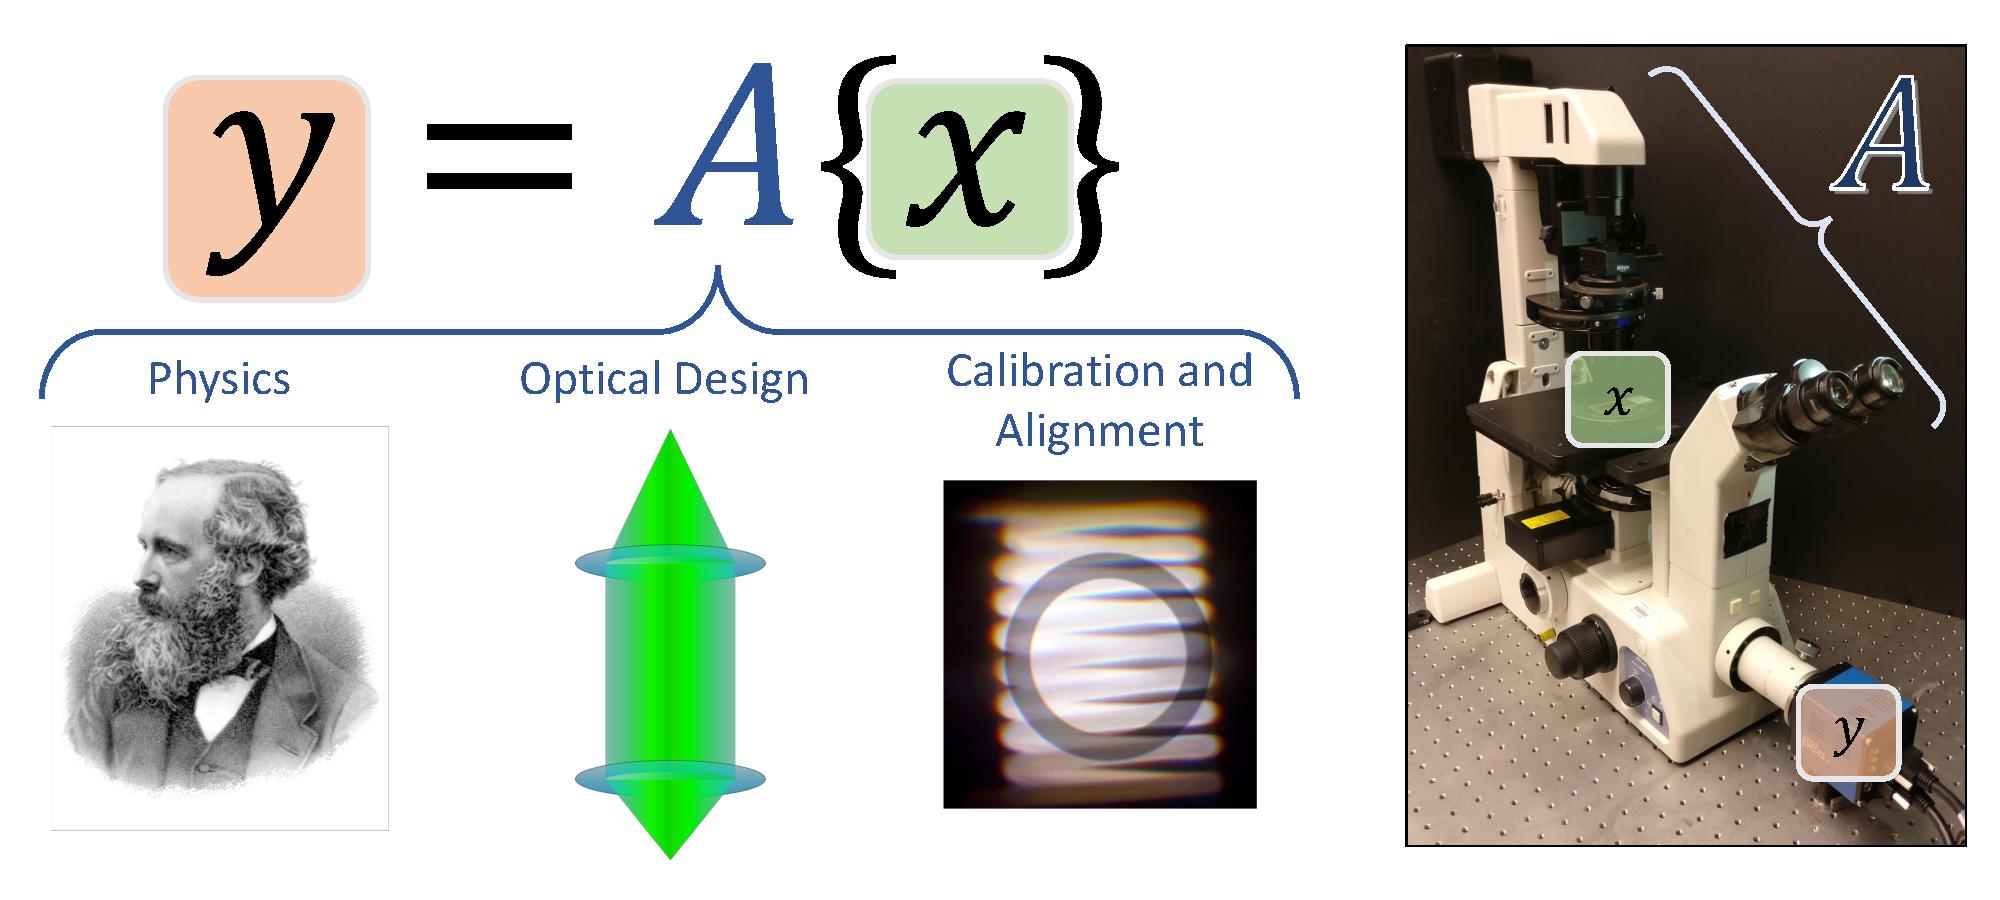
\includegraphics[width=0.95\textwidth]{figures/fig_intro_comp_imaging.pdf}
    \label{fig:intro_overview}
    \caption{Overview of Computational Imaging. The forward model $\op{A}$ is a function of the physical properties of light, the optical system design, and (mis)calibration of the system. An image of a Nikon TE300 microscope used in this work is provided for context.}
\end{figure}

The concept of using computational tools to simulate and invert optical imaging systems was developed soon after the emergence of computers, based on the mathematical framework which was developed prior to this time. Recently, the field of computational imaging has expanded considerably due to increasing availability of computing power and digital sensing hardware. In modern microscopes, digital cameras allow the detection of the intensity of an optical field using a grid of photodetectors, which digitize the optical field and facilitate computational imaging reconstructions on a host computer. As graphical processors (GPUs) have become faster and more widely available, computational algorithms have likewise accelerated both in speed and scale.

An early example of computational imaging was the application of a cubic phase plate at the microscope pupil, which provides drastically increased depth of field but produces a highly distorted image. Since these distortions are known, however, the original image with extended depth of field can be deconvolved using knowledge of the system's point spread function (PSF)\cite{Dowski:95}. Since these early works, computational microscopy has ballooned due to the widespread availability of computing hardware and software tools for simulating optical systems and performing quantitative analysis. Prominent examples include super-resolution methods such as structured illumination~\cite{gustafsson2000surpassing, gustafsson2005nonlinear}, which enhances resolution by projecting a pattern onto the sample, localization microscopy~\cite{betzig2006imaging, Rust:06}, which employs statistical analysis to localize sparse fluorophores using temporal dynamics, and both conventional~\cite{rodenburg2004phase} and Fourier~\cite{Zheng2013} ptychography. Three-dimensional imaging has likewise become a powerful for imaging three dimensional biological quantities and becomes absolutely necessary for high-$NA$ imaging of thick samples which encounter multiple scattering. Various approaches have been proposed, including deconvolving focal stacks~\cite{agard1984optical}, light-field microscopy~\cite{broxton2013wave, Ng2005}, point-spread function engineering~\cite{pavani2008three}, as well as diffraction tomography~\cite{wolf1969three, kim2014diffraction, maleki1992tomographic}. In addition, computational imaging has been widely used for quantitative phase imaging, using interferometry~\cite{Popescu2006,kim2014diffraction, Bhaduri:12}, Off-axis holography~\cite{Witte:12}, commercial add-ons~\cite{phasics,bon2012method}. Another add-on option uses two cameras to capture defocused images which can then be used to solve the Transport of Intensity Equation (TIE)~\cite{allman2005optical}. Alternatively, if chromatic aberrations are large enough, they can enable single-shot color TIE~\cite{wallerColorTIE} without any hardware changes.

Reconstruction algorithms vary considerably based on the desired application and acquisition strategy, but most build upon theoretical abstractions provided by the Fourier optics model. The seminal text on imaging using Fourier theory to analyze imaging systems was published in 1968~\cite{goodman:68} which produced the framework which enables many common computational techniques such as deconvolution, holography, and the free-space propagation of an electric field. The Fourier optics description is especially useful for an optical system configured as a telecentric ($4f$) system:

\begin{figure}[tbh]
\centering
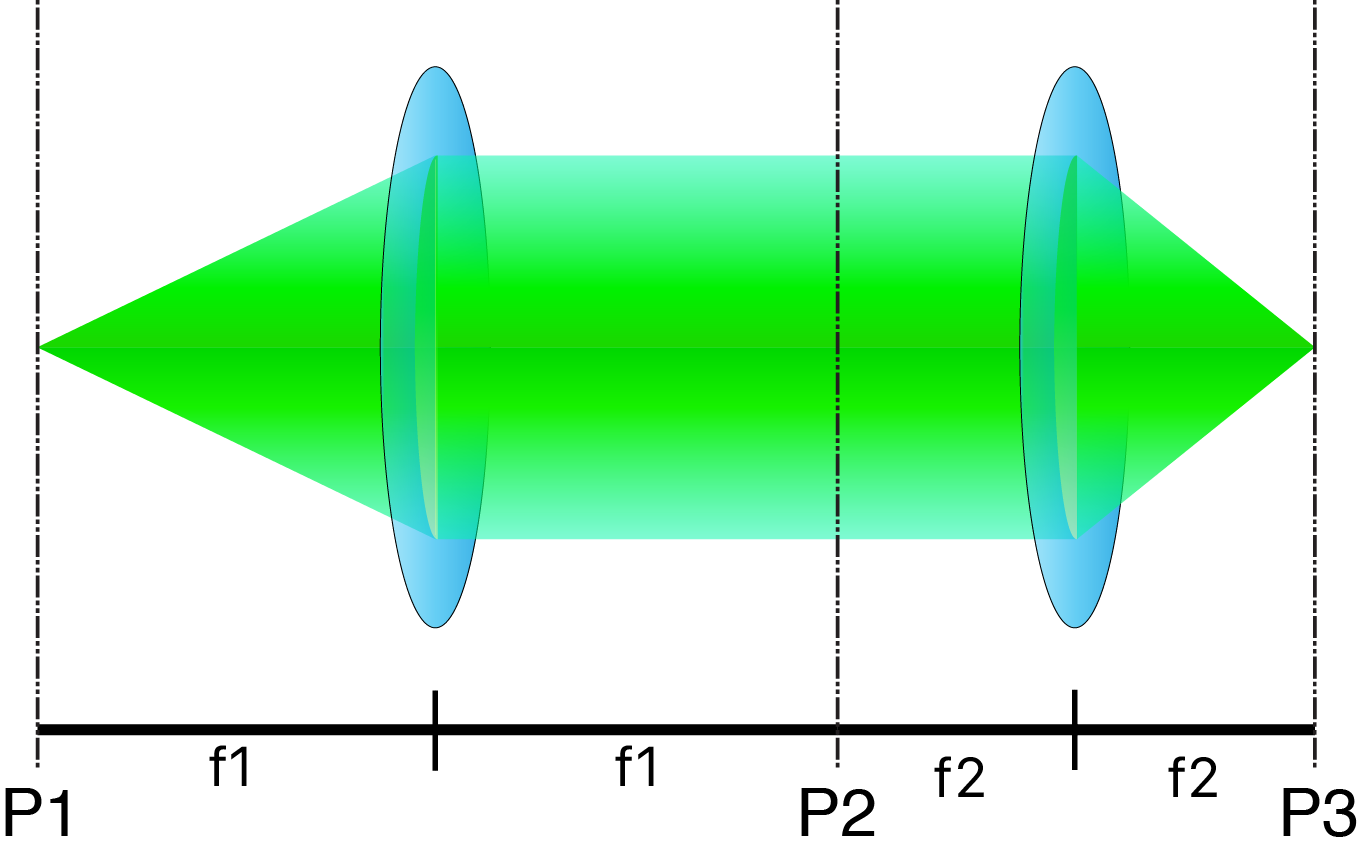
\includegraphics[width=0.4\textwidth]{intro-4f.png}
\caption{\label{fig:4f} Schematic of a 4$f$ optical system}
\end{figure}

\noindent In this system, the lenses in this system operate as forward and inverse Fourier transform operators on the input optical field at (P1) as it propagates through the pupil plane (P2) to the image plane (P3). In this configuration, the electric field at position P2 can be modeled as the Fourier transform of P1, which is often occupied by an aperture stop (circular low-pass filter) to limit the NA of the objective. This stop defines the resolution of the optical system and can be used to reduce aberrations and prevent aliasing of the optical signal at the camera plane.

In most cases the propagation and refraction of light can be modeled using a small number of linear and non-linear operations and may be accurately simulated using linear algebra software packages such as \texttt{numpy}. With knowledge of this forward model, an inverse problem may be formed to recover the object without any distortions imposed by the imaging system (provided the information is still present in the measurement). In computational imaging these distortions are carefully designed to reveal contrast in ways a conventional system cannot, enabling the recovery of high-dimensional or high-resolution information using computation after an acquisition in performed. Many imaging inverse problems share a common standard form:

\begin{equation}\label{eq:intro_inverse_problem}
\begin{aligned}
& \hat{\vec{x}} = \underset{\vec{\vec{x}}}{\text{argmin}}
& & ||\op{A}\{\vec{x}\} - \vec{y} ||_2^2
\end{aligned}
\end{equation}

Where $\vec{x}$ represents the variable of interest (generally the object), $\op{A}\{\cdot\}$ is the mathematical operation describing the optical system, $\vec{y}$ is the measured intensity, and $\hat{\vec{x}}$ is an estimate of the object $\vec{x}$. The forward operator $\op{A}\{\cdot\}$ is normally formed based on the physics of the optical systems, need not be linear or represented by a matrix.

The goal of a computational imaging system is to invert the forward operator $\op{A}\{\cdot\}$ in a way which minimizes the distance between the object estimate distortions of the forward-inversion process ($||\hat{\vec{x}} - \vec{x}||_2^2$). If $\op{A}\{\cdot\}$ is linear, is can be inverted in a closed-form solution using the Moore-Penrose Pseudo-Inverse~\cite{moore1920reciprocal}, or with an iterative method such as gradient descent. If $\op{A}\{\cdot\}$ is non-linear but smooth, it must be inverted iteratively using analytic expressions for each regularization. If $\op{A}\{\cdot\}$ is non-smooth, it can, in some cases, still be inverted using iterative soft-thresholding method such as FISTA~\cite{beck2009fast}.

In general, linear problems (characterized by satisfying the relationship $\op{A}\{\vec{a} + \vec{b}\} = \op{A}\{\vec{a}\} + \op{A}\{\vec{b}\} $) are much easier to invert and solve, having lower memory requirements and complexity as well as a direct inverse. Linear convolution operators are particularly common for telecentric imaging systems. When a convolution is well-posed, it may be efficiently inverted using a FFT-based deconvolution algorithm~\cite{cooley1965algorithm}, which has complexity $N \log(N)$ as opposed to $N^2$ for normal operators.

The performance of inversion processes may be improved by adding regularization term to penalize certain undesirable characteristics of the signal, such as noise. The most commonly used regularization method is Tikhonov (or $\ell_2$) regularization~\cite{tikhonov1943stability} which enforces a prior on the total energy of a system. Tikhonov regularization is equivalent to adding an additional $\ell_2$ term to Eq.~\ref{eq:intro_inverse_problem}:

\begin{equation}\label{eq:intro_tikhonov}
\begin{aligned}
& \hat{\vec{x}} = \underset{\vec{x}}{\text{argmin}}
& & ||A\{\vec{x}\}-\vec{y} ||_2^2 + \alpha||\vec{x}||_2^2
\end{aligned}
\end{equation}

\noindent where $\alpha$ is a tuning parameter which represents the weight of the Tikhonov prior (normally set to $\frac{1}{SNR}$). If $\op{A}\{\cdot\}$ is linear and can be represented as a matrix, Eq.~\ref{eq:intro_tikhonov} can be directly inverted using a closed-form expression:

\begin{equation}
    \hat{\vec{x}} = ((\mat{A}^H \mat{A})^{-1} + \alpha \mat{I})\mat{A}^H \vec{y}
\end{equation}

\noindent where $\mat{A}$ is the matrix form of $\mat{A}\{\cdot\}$ and $\mat{I}$ is the identity matrix with the same dimensions as $\mat{A}^H \mat{A}$. This closed-form solution makes Tikhonov regularization popular for many inverse problems, although the total energy prior may not be accurate in all cases.

A second common class of priors enforce sparsity of the object in some domain. Mathematically the $\ell_0$ "norm" returns the number of non-zero elements of the input. This norm is non-convex, however, requiring a large combinatorial search which is intractable for most problems~\cite{candes2008enhancing}. As a proxy, the $\ell_1$ norm is conventionally employed as a convex, though non-smooth alternative~\cite{taylor1979deconvolution}. When coupled with a generalized sparsifying operator $\op{W}\{\cdot\}$ and a differential forward model $\op{A}\{\cdot\}$, this problem is convex, and can be written as:

\begin{equation}\label{eq:intro_sparse}
\begin{aligned}
& \hat{\vec{x}} = \underset{\vec{x}}{\text{argmin}}
& & ||\op{A}\{x\}-\vec{y} ||_2^2 + \alpha||\op{W}\{\vec{x}\}||_1
\end{aligned}
\end{equation}

Because the regularization term is non-smooth, iterative solvers must be used to recover the optimal $\hat{\vec{x}}$. When $\op{W}$ is a unitary function $\mat{w}$ (or the identity matrix), a solver implementing proximal gradient descent using soft-thresholding may be used to minimize this objective function, such as FISTA~\cite{beck2009fast}, ADMM~\cite{boyd2011distributed}, or TwIST~\cite{bioucas2007new}. In general, $\mat{W}$ can be any unitary transform, including the Fourier transform  or Wavelet Transform, or a learned unitary operator which is optimized using a machine-learning framework~\cite{ravishankar2013learning}. In all of these cases, the optimal $\hat{\vec{x}}$ may be recovered by performing many iterations of proximal gradient descent:

\begin{equation}
    \vec{x}^{k+1} = \mat{W}^H prox_{\alpha}(\mat{W} (\vec{x}^{k} - \alpha \nabla_{\op{A}\{\vec{x}\}} (\op{A}\{\vec{x}\} - \vec{y})))
\end{equation}

In the case where $\mat{W}$ is not unitary, the above relationship does not hold, and other proximal methods must be used. One prominent example is total-variation regularization (TV), which enforces sparsity of the image gradients~\cite{rudin1992nonlinear}. TV regularization can be implemented using ADMM~\cite{wahlberg2012admm}, FISTA~\cite{beck2009fast}, or using soft-thresholding on wavelet coefficients~\cite{kamilov2012wavelet}, although it is known to create a "cartoon-like" effect for high $\alpha$ values.

\section{Noise in Computational Microscopy Systems}\label{sec:intro_noise}
All measurements contain noise from various sources, including photon quantization, camera electronics. In general, these noise sources can be additive or multiplicative, and may take on a variety of statistical profiles including Gaussian and Poisson distributions. In this dissertation, we generally assume the presence of an additive, Gaussian noise term $\vec{\eta}$ with zero-mean, and variance $\sigma_{\vec{\eta}}$, which is added to each measurement made under a general forward operator $\op{A}\{\cdot\}$:

\begin{equation}\label{eq:intro_forward_model}
    \vec{y} = \op{A}\{\vec{x}\} + \vec{\eta}
\end{equation}

This approximation is generally valid for measurements made with more than 10 photon counts, which includes every case presented in this dissertation (including fluorescence imaging). The effect of this noise on image quality is generally represented as the signal-to-noise ratio (SNR). Here, we use the common imaging SNR definition:

\begin{equation}
    \label{eq:intro_snr}
    SNR = \frac{\bar{\vec{y}}}{\sigma_{\vec{\eta}}}
\end{equation}

\noindent where $\sigma_{\vec{\eta}}$ is the standard deviation of the noise term. When inverting the forward operator $\op{A}\{\}$ to recover $\vec{x}$, the presence of $\vec{\eta}$ will lead to error in the measurements compared to the ground truth. Take, for example, if $\op{A}$ can be represented as a matrix $\mat{A}$, the Moore-Penrose pseudoinverse of the object is given by:

\begin{equation}\label{eq:intro_noise_inverse}
        \hat{\vec{\vec{x}}} = (\mat{A}^H \mat{A})^{-1} \mat{A}^H y = (\mat{A}^H \mat{A})^{-1} \mat{A}^H \mat{A} \vec{x} + (\mat{A}^H \mat{A})^{-1} \mat{A}^H \vec{\eta} = \vec{x} + (\mat{A}^H \mat{A})^{-1} \mat{A}^H \vec{\eta}
\end{equation}

Based on Eq.~\ref{eq:intro_noise_inverse}, the root-mean-squared error (RMSE) between $\hat{\vec{x}}$ and the true $\vec{x}$ is $(\mat{A}^H \mat{A})^{-1} \mat{A}^H \vec{\eta}$. Taking the covariance of this term, we can find an expression for the covariance of the error term in the reconstruction:

\begin{equation}\label{eq:intro_noise_covariance}
    \mat{\Sigma}_{\mat{A}^{\dagger}\vec{\eta}} = (\mat{A}^H \mat{A})^{-1} \mat{A}^H \sigma_{\vec{\eta}}^2 \mat{A} (\mat{A}^H \mat{A}) ^{-H} = \sigma_{\vec{\eta}}^2 (\mat{A}^H \mat{A})^{-1} \mat{A}^H  \mat{A} (\mat{A}^H \mat{A}) ^{-H} = \sigma_{\vec{\eta}}^2 (\mat{A}^H \mat{A}) ^{-H}
\end{equation}

The main result of Eq.~\ref{eq:intro_noise_covariance} is that the inversion process re-weighs the spectrum of the original Gaussian white noise $\vec{\eta}$. When $\mat{A}$ has an $\ell_2$ operator norm of 1, the minimum singular value of $\mat{A}$ defines the maximum noise amplification, while the sum of the inverse singular values defines the total RMSE:

\begin{equation}\label{eq:intro_noise_amplification}
    \sigma_{\mat{A}^{\dagger}\vec{\eta}} = \sigma_{\vec{\eta}} \sqrt{\mat{\Sigma}_{i=0}^N{\frac{1}{\sigma_i^2\{\mat{A}\}}}} = \sigma_{\vec{\eta}} \sqrt{Tr\{(\mat{A}^H \mat{A})^{-1}\} / N}
\end{equation}

\noindent where $N$ is the length of $\vec{x}$ and $\sigma_i^2 \{\mat{A}\}$ represents the $i^{th}$ singular value of $\mat{A}$. This definition is consistent with~\cite{agrawal2009optimal}. This relationship between the singular values of $A$ and the amplification of $\vec{\eta}$ enables a closed-form relationship to the reconstruction signal-to-noise ratio ($SNR_{recon}$) of a measurement $\vec{y}$, defined as:

\begin{equation}\label{eq:intro_snr_recon}
SNR_{recon} = \frac{\bar{\vec{y}}}{\sigma_{\mat{A}^{\dagger}\vec{\eta}}} = \frac{\bar{\vec{y}}}{\sigma_{\vec{\eta}} \sqrt{\mat{\Sigma}_{i=0}^N{\frac{1}{\sigma_i^2\{\mat{A}\}}}}}
\end{equation}

Where $\bar{\vec{y}}$ is the mean signal of the measurement as in Eq.~\ref{eq:intro_snr_recon}. From this relationship, it becomes clear that the deconvolution process will reduce the $SNR$ by a factor:

\begin{equation}\label{eq:intro_dnf}
    f = \sqrt{\mat{\Sigma}_{i=0}^N{\frac{1}{\sigma_i^2\{\mat{A}\}}}}
\end{equation}

Where $f$ is the deconvolution noise factor (DNF). This result is particularly useful for convolutional forward operators, where the singular values of $A$ can be computed quickly and efficiently from the Fourier coefficients of the convolution kernel $h$ due to the circulant structure of $A$. This analysis of RMSE amplification is equivalent to A-optimal design~\cite{chernoff1953locally}, which is used here due to strict compatibility with the definition of imaging snr (Eq.~\ref{eq:intro_snr}).

\begin{figure}[tbh]
\centering
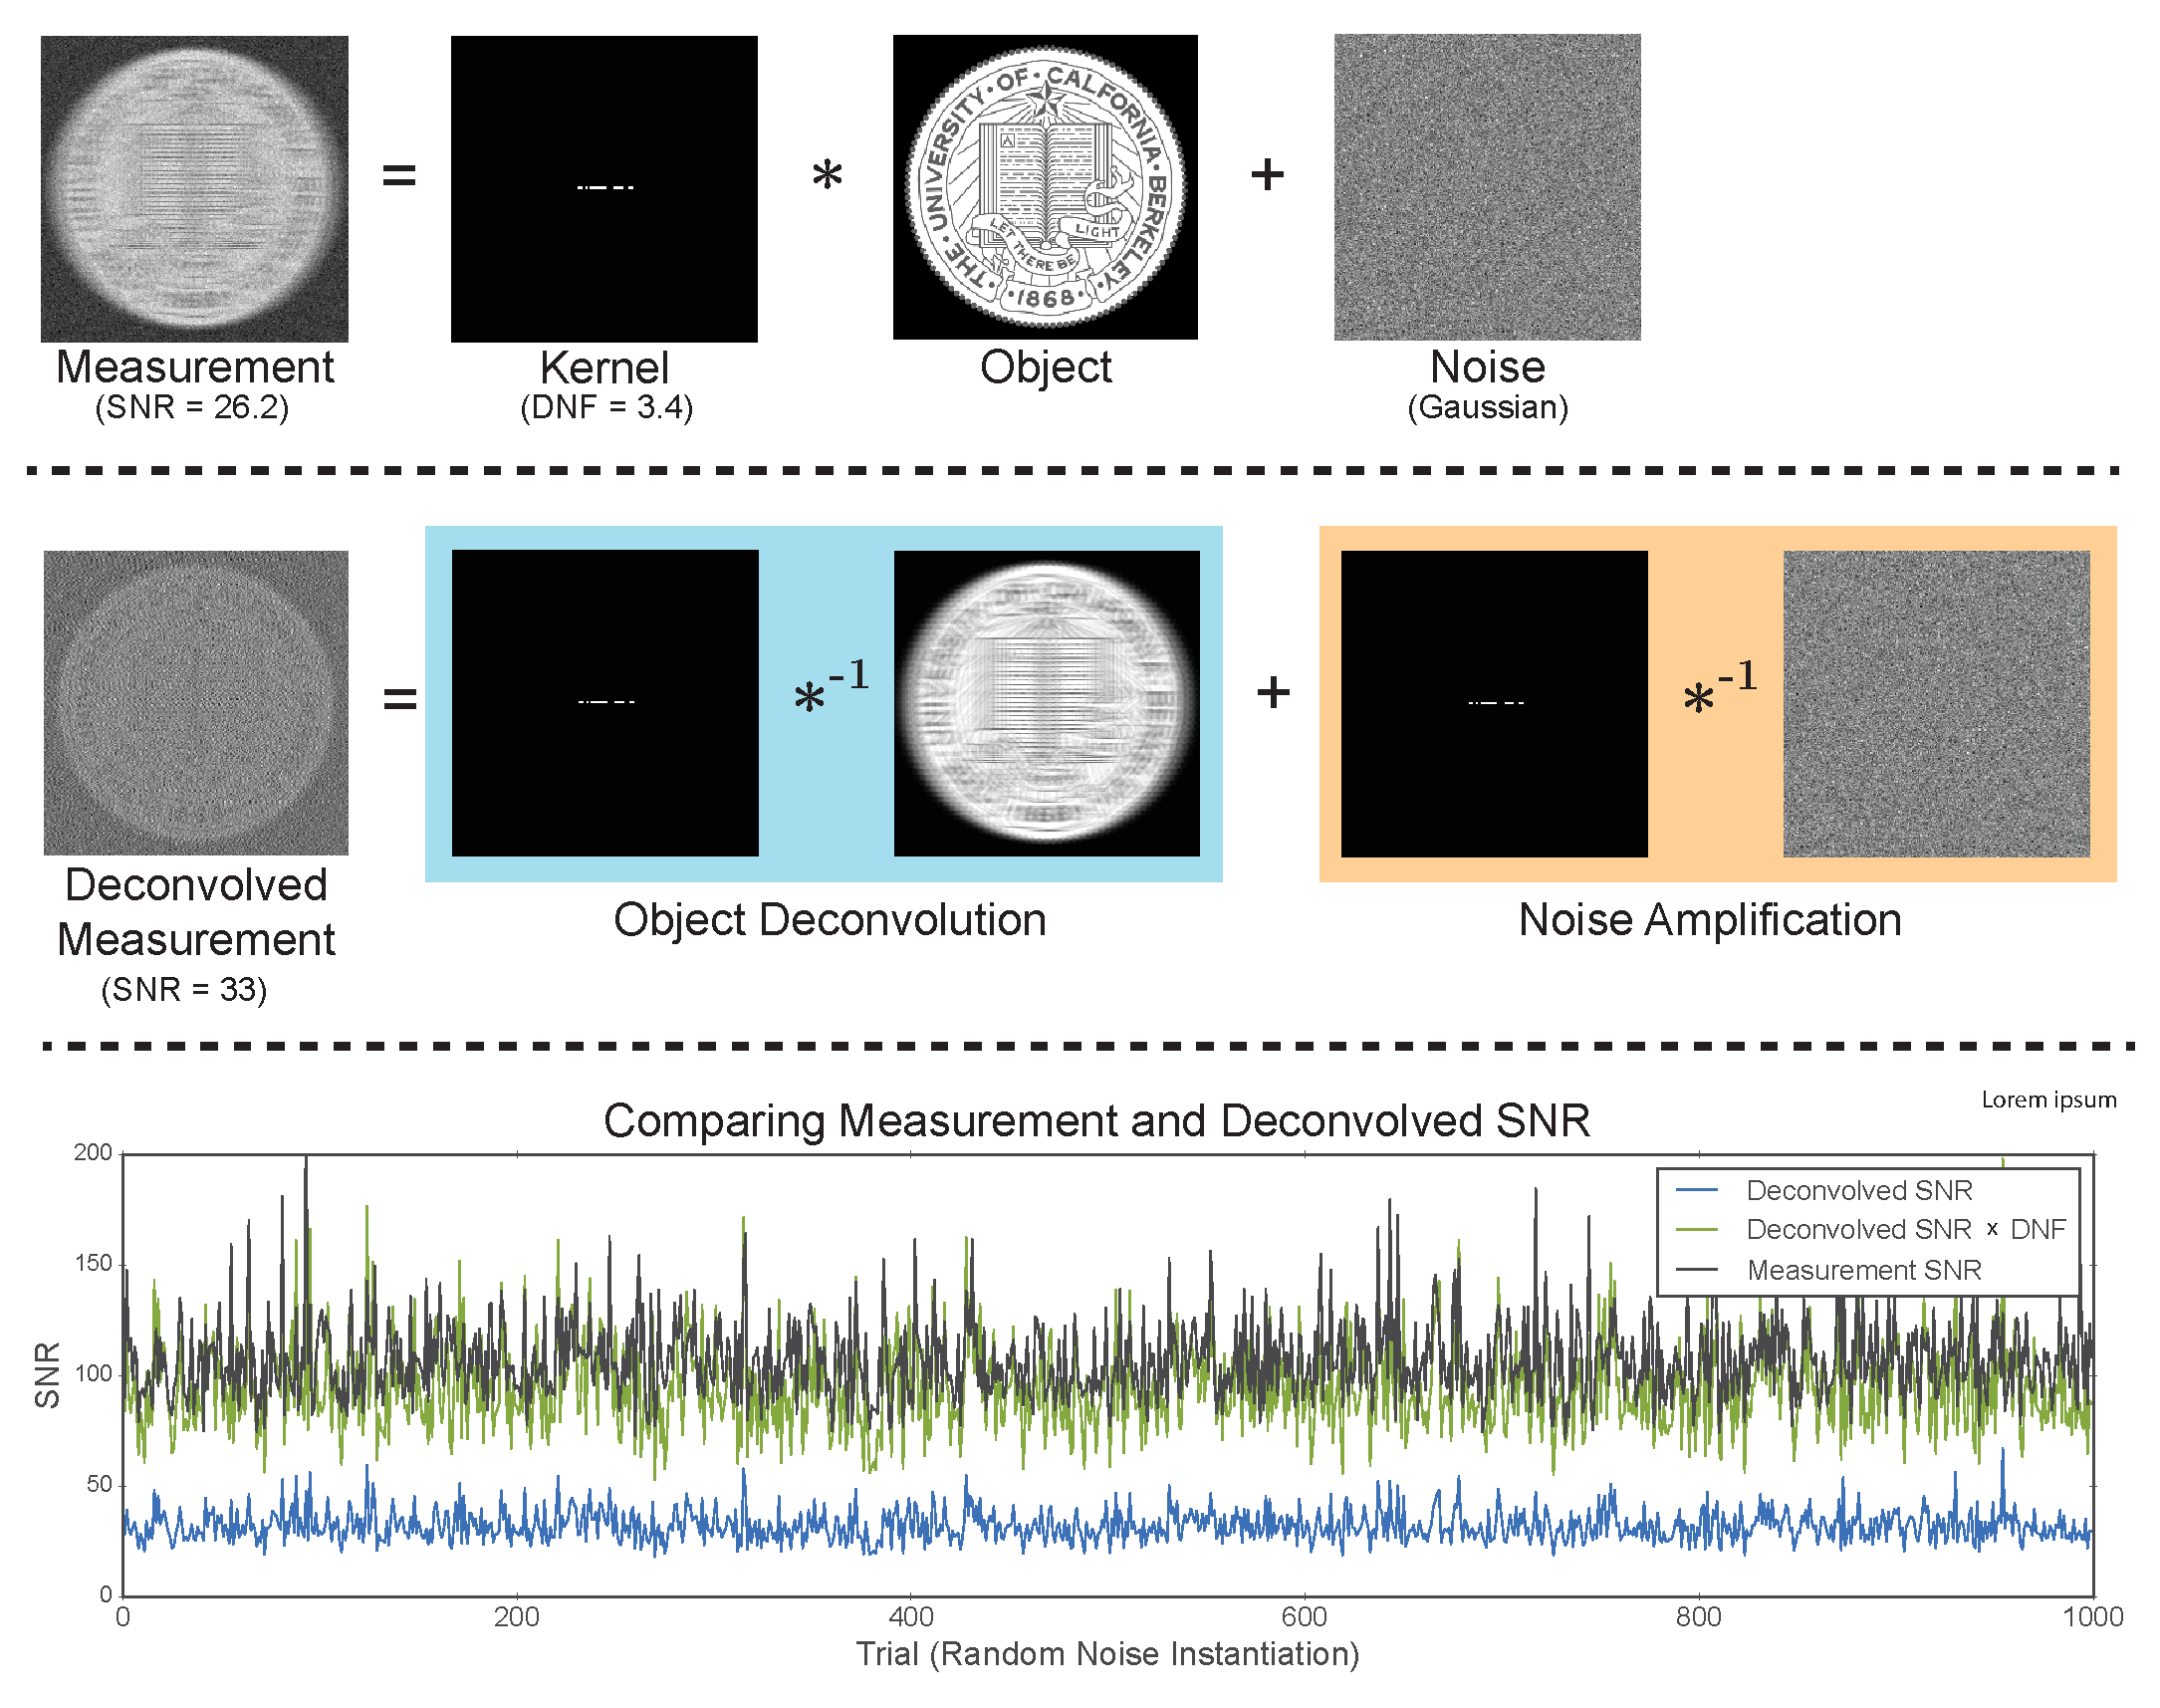
\includegraphics[width=\textwidth]{figures/fig_intro_dnf.pdf}
\caption{\label{fig:intro:dnf} Simulation of a convolutional forward model and verification of DNF calculations. Top row shows forward modal with additive Gaussian noise, while the middle row shows the deconvolution of the same measurement, separated into object deconvolution and noise amplification terms. Bottom row shows the measurement and reconstruction SNR across 1000 random generations of the Gaussian white noise term, overlaid with the multiplication of the reconstruction SNR multiplied by the DNF as a verification. The operators $*$ and $*^{-1}$ represent 2D convolution and deconvolution, respectively.}
\end{figure}

As a demonstration of this relationship, we simulated a convolutional forward model with additive Gaussian noise, and performed deconvolution of the noisy measurement. These results show that the DNF provides a very close scalar relationship between measurement SNR and deconvolved SNR, which is illustrated by comparing the estimated measurement SNR (deconvolved SNR multiplied by the DNF) to the original measurement SNR. Small discrepancies between the expected and predicted SNR calculations are likely due to sampling error, since we evaluate the noise standard deviation across a 20-pixel square in the top left corner of each image, rather than the full image (to avoid including the standard deviation of the object in our SNR calculation). These relationships are used in both Chapter~\ref{ch:phase} and Chapter~\ref{ch:highthroughput} for analyzing the noise propagation of linear forward models.

\section{Coded Illumination for Optical Microscopy}


Since the 17$^{th}$ century, microscopes have employed some sort of light source to illuminate a specimen, from candles to semiconductor light sources. In this dissertation, we explore, through both theory and demonstration, the use of programmable LED sources for microscopy, replacing conventional sources such as halogen lamps. These sources enable both fast switching of qualitative contrast methods~\cite{Zheng2011, albeanu2008led} as well as the capability to perform quantitative reconstructions of the complete complex field of the sample~\cite{Tian3dDpc, Zheng2013, tian2015quantitative}.

Contrast in optical microscopy is conventionally obtained in a variety of ways - for purely absorptive samples, bright field microscopy images the light that is attenuated by the sample by illuminating within the range of angles defined by the numerical aperture ($NA$) of the objective. Conversely, dark field microscopy uses illumination from angles outside of the illumination $NA$, imaging only light that is scattered or "bent" by a refractive medium such as water. Rather than relying on expensive illumination hardware to block transmitted light at the pupil plane, the simple addition of an LED array enables both of these modalities by dynamically changing the pattern via software~\cite{Zheng2011, zijiMulti}.

In addition to qualitative phase contrast, computational illumination using a LED array enables quantitative phase recovery through with an LED array microscopy involves methods such as Fourier ptychography Ptychography~\cite{Zheng2013, Tian14} and differential phase contrast~\cite{mehta2009quantitative,
tian2015quantitative}, enabling the measurement of the dry mass of many aqueous biological samples~\cite{popescu2008imaging, popescu2008optical}.

In the following chapters, I will describe several novel applications and of coded illumination in optical microscopy, fabrication methods for coded illumination devices, and self-calibration techniques for the aforementioned methods, Fig.~\ref{fig:intro_system_dome} shows the system which was used in most experiments presented in this dissertation. Chapter~\ref{ch:phase} describes methods for qualitative and quantitative phase recovery, including single-shot quantitative phase imaging method which uses partially coherent color illumination to recover the complete optical field of an object from a single measurement. In addition, we perform a SNR-based optimization of LED patterns for linearized phase retrieval using a partially coherent source. Chapter~\ref{ch:highthroughput} describes a novel method for recovering a large field-of view with high SNR by introducing motion deblur during each capture and use a motion deblurring algorithm to recover the static object. We demonstrate the performance of this technique for both brightfield imaging and fluorescence imaging and provide an analysis of optimal acquisition strategy in terms of common system parameters such as camera noise level and illumination power. In Chapter~\ref{ch:fabrication}, we describe the fabrication of several prototypes used for coded illumination, including a programmable domed LED array, LED sources for high-throughput imaging, as well as Computational CellScope, a prototype device which uses a programmable domed LED illumination to perform quantitative phase imaging, digital refocusing, and multi-contrast imaging in a portable (smartphone-based) form factor. Chapter~\ref{ch:selfcal} describes self-calibration techniques for quantitative phase imaging, including LED position recovery for LED domes and aberration recovery using a linearized model. These methods are essential for practical implementation of many quantitative phase imaging techniques. Chapter~\ref{ch:conclusion} concludes this dissertation on quantitative microscopy using coded illumination and provides future extensions of the work presented in the previous chapters.

\begin{figure}[bh]
    \centering
    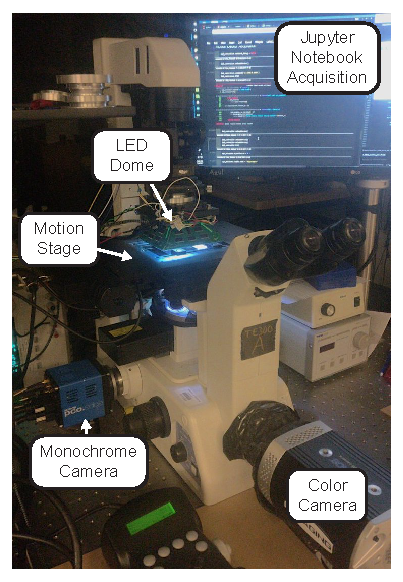
\includegraphics[width=0.7\textwidth]{figures/fig_intro_dome_system.pdf}
    \label{fig:intro_system_dome}
    \caption{Nikon TE300-based system used for most experiments presented in this dissertation consisting of a digital camera, programmable LED illumination source, and mechanical motion stage. Here, a quasi-domed illuminator is mounted in place of the conventional optical condenser, although this may be replaced with a single LED high-throughput imaging.}
\end{figure}

\chapter{Single-Shot Quantitative Phase Retrieval}

\section{Quantitative Phase Imaging}
Quantitative Phase Imaging (QPI) involves recovering the amplitude and phase, or complex field, of a sample. In contrast to \emph{qualitative} phase imaging methods, such as Zernike phase contrast (PhC)\cite{zernike1955discovered}) and Differential Interference Contrast (DIC)\cite{smithDIC}, \emph{quantitative} methods recover the phase delay caused by the sample, decoupled from absorption information. Modifications of PhC~\cite{yun2010system} and DIC~\cite{CuiYangTearney2011} can make these setups quantitative, at a cost of requiring multiple images. More commonly, QPI methods use interferometry with coherent illumination and a reference beam~\cite{Popescu:06,Wang:11,Bhaduri:12}, making them expensive and sensitive to misalignment and vibrations.

Differential Phase Contrast (DPC)~\cite{Hamilton1984a,mehta2009quantitative,Tian14,tian2015quantitative} is a partially coherent QPI technique that requires multiple images. Each is captured using a different asymmetric half-circle source pattern, which shifts the sample's spectrum in Fourier space. Thus, a half circle source and its complement will cause the pupil function to crop opposite sides of the sample's spectrum. Since imaginary information is encoded in Fourier asymmetry, these images can be used to recover phase. Assuming a linearized model for a weakly scattering sample, the inverse problem becomes a single-step deconvolution process~\cite{mehta2009quantitative,tian2015quantitative}. DPC recovers both amplitude and phase with resolution up to the incoherent resolution limit ($2\times$ better than coherent methods). Practically, the illumination switching can be done quickly and at low cost with an LED array~\cite{Tian14,zijiMulti,tian2015quantitative}. At least two complementary source patterns are required, but generally 4 patterns (top, bottom, left, right half-circles) are used to avoid missing frequencies. The DPC method was recently extended to color multiplexing~\cite{lee2015color}, where the 4 source patterns were encoded into two images by using a color camera in combination with a color LED array. Similarly, color photometric stereo has been used for retrographic surface profiling of large objects using off-axis color illumination in reflection mode~\cite{johnson2009retrographic}.

Amongst the wide array of existing QPI methods, several are single-shot techniques. Off-axis holography interferes the sample beam with a tilted reference beam, then recovers phase by Fourier filtering~\cite{Witte:12}. Parallel phase-shifting can spatially multiplex several holograms within a single exposure via an array of polarizers~\cite{2004singleshotPSDH}. And single-shot QPI add-ons based on amplitude gratings work with commercial microscopes, replacing the traditional camera module~\cite{phasics,bon2012method}. Another add-on option uses two cameras to capture defocused images which can then be used to solve the Transport of Intensity Equation (TIE)~\cite{allman2005optical}. Alternatively, if chromatic aberrations are large enough, they can enable single-shot color TIE~\cite{5714248} without any hardware changes. All of these methods require the some spatial or temporal coherence, limiting resolution, but provide camera-limited frame rates.

\begin{figure}[tbh]
\centering
\includegraphics[width=\textwidth]{cdpc-Fig1.pdf}
\caption{\label{fig:hardware}
Single-shot color Differential Phase Contrast (cDPC) microscopy. a) Installation in Nikon TE300 microscope condenser turret. b) CAD model and image of fabricated cDPC insert.c) Optical schematic of a brightfield microscope with a cDPC color filter placed at the back focal plane of the condenser in K\"{o}hler configuration. d) Reconstruction: the captured color image is separated into its RGB components, which are then used to recover two unknowns (amplitude and phase) via a well-posed linear deconvolution. The sample is a micro-lens array (Fresnel Technologies 605). }
\end{figure}

\section{Color-Multiplexed Differential Phase Contrast (cDPC) }
To improve temporal resolution of a DPC system without compromising spatial resolution a multiplexing configuration is necessary to make the problem well-posed. The proposed alternative method, color Differential Phase Contrast (cDPC), requires only a \emph{single} color image for multiplexing source patterns. In this method, the source is discretized into three color channels which are used to display three different half-circle source patterns. It is important to note that while the original DPC algorithm presented in \cite{tian2015quantitative} requires 4 images, the proposed method only requires 3, since the 4th source configuration can be synthesized by taking the sum of two images acquired with opposite half-circle illuminations (a synthetic brightfield image) and subtracting that of a 90 degree rotated half-circle source. In early prototypes the color source pattern pattern was implemented in an LED array microscope, which offers many imaging modalities in one platform~\cite{Tian14,zijiMulti,tian2015quantitative,Ma:15,Phillips15, Zheng2011, Zheng2013}. However, the proposed configuration does not require a dynamic source, making it possible to use a static multi-color filter placed in the condenser back focal plane, assuming K\"{o}hler illumination. Both configurations simplify hardware and reduce costs significantly as compared to phase contrast or DIC, while providing quantitative phase, which is more general and can be used to synthesize both of the aforementioned methods digitally~\cite{JMI:JMI1027}.

\subsection{Hardware Design}
As in conventional DPC, this method requires measurements of the sample illuminated by known asymmetric sources. In cDPC, however, we make use of the microscope's existing condenser unit, which has a turret commonly used for phase contrast inserts or DIC prisms. This intermediate plane can usually be accessed easily by removing the mechanical inserts. Taking advantage of this configuration, a simple 3D printed color filter was designed and fabricated that can be placed in the condenser turret of a Nikon TE300 microscope (Figure~\ref{fig:hardware}a).

The filter prototype consists of Polyethylene Terephthalate (PET) color filters (Lee Filter, Inc.) laser cut to size and installed into a 3D printed insert designed to fit our microscope. Narrow bandwidth illumination filters (e.g. multi-layer coated glass) would separate colors better, but suffer from low light throughput and high cost. Therefore, inexpensive and easy-to-cut PET film filters were used; the resulting cross-talk between color channels will be accounted for in post-processing, described below.

The total cost of raw materials is approximately $\$30$ and filters were produced quickly with a 3D printer and laser cutter. One filter is shown in Figure~\ref{fig:hardware}b; it was installed in the condenser turret of an inverted microscope (Figure~\ref{fig:hardware}a), replacing one of the removable phase contrast (Ph1, Ph2 or Ph3) inserts.
\subsection{Calibration}
\label{Calibration}

Ideally, the color filters would provide perfect separation of the three source patterns into the three color channels. In reality, both the illumination and camera color channels have cross-talk between the desired wavelengths. To account for this, system calibration is separated into two separate steps: detection-side and illumination-side.

Illumination-side calibration corrects for the relative spectral transmittance of each of the source color filters. The illumination pattern simultaneously encodes three half-circle sources, one each for the RGB color channels. Red and green are opposite half-circles, and blue is rotated by 90 degrees relative to the others. Where the blue and green patterns overlap, a cyan filter (blue + green) was used. Where the blue and red patterns overlap, a purple filter (blue + red) was used. Hence, the final filter design actually contains four quadrants having red, green, cyan and purple filters (see Fig.~\ref{fig:transferfunctions}).

\begin{figure}[tbh]
\centering
\includegraphics[width=0.8\textwidth]{cdpc-Fig2.pdf}
\caption{\label{fig:transferfunctions}
Transfer functions for amplitude and phase contrast in each cDPC color channel. Left: Spectral contribution of each illumination filter as captured by the camera's Bayer pattern. The following columns show the components of the amplitude and phase transfer functions in the spatial frequency domain and the source represented in each image.  Bottom row: sum of each column, representing the calibrated and scaled source and the total coverage of amplitude and phase transfer functions, respectively. }
\end{figure}

When filtered by the sensor Bayer pattern, the filter spectrum bases are not orthogonal. This can be seen in the spectra of each PET film after capture with a color camera (left column of Fig.~\ref{fig:transferfunctions}). The result is an undesirable loss of asymmetry in the source that reduces phase SNR. However, it is possible to account for the asymmetry during reconstruction by modeling the source patterns as in Fig.~\ref{fig:transferfunctions}.

Detection-side calibration accounts for spectral cross-talk of the camera color channels. Standard RGB Bayer filters do not provide perfect discrimination between RGB wavelengths, but coupling artifacts can be removed by calibration. Given the pixel values from the raw color image with an RGBG Bayer filter ($I_r$, $I_{g1}$, $I_{g2}$, $I_b$), it is possible to solve for the decoupled color image ($I_R$, $I_{G}$, $I_{B}$) that would be obtained if the sample were illuminated with a single color, according to the following equation,

\begin{equation}
\label{eq:couplingmatrix}
\begin{bmatrix}
I_{r} \\
I_{g1}\\
I_{g2}\\
I_{b}
\end{bmatrix}
 =
 C
 \begin{bmatrix}
I_{R} \\
I_{G}\\
I_{B}
\end{bmatrix}.
\end{equation}

\noindent  The matrix $C$ is a 4$\times$3 calibration matrix describing the coupling between each color channel. It is generated by filtering the broadband source with each filter independently, then measuring the relative red ($I_R$), green ($I_G$) and blue ($I_B$) read-outs to populate the corresponding column vectors of the $C$ matrix. The ratio between the intensities of each flat-field image at each detection channel provides a linear weighting of the contribution of each source to the color measurement. Once $C$ has been measured once, it can be used to pre-process all later measurements by solving Eq.~\eqref{eq:couplingmatrix}. This step is important for reducing artifacts in the phase results.

Another important step for cDPC is to account for wavelength-dependent changes in phase and spatial frequency. DPC recovers absorption ($\mu$) and phase ($\phi$) information from intensity measurements. These quantities are defined as:

\begin{equation}
\label{eq:absorption_phase}
\mu = \frac{2\pi}{\lambda_0} \alpha d,\ \phi = \frac{2\pi}{\lambda_0} n d,
\end{equation}

\noindent where $\lambda_0$ is a reference wavelength, $d$ is the thickness of the sample, $n$ represents refractive index and $\alpha$ indicates absorption coefficient. Absorption and phase transfer functions are determined by illumination numerical aperture (NA), objective NA and illumination wavelength~\cite{tian2015quantitative}. In the proposed color-multiplexed DPC method, the transfer functions must also consider the change in wavelength of each color channel. Phase ($\phi$) depends on which wavelength is used. By assuming no dispersion in the sample, it is possible to use Eq.~\eqref{eq:absorption_phase} to synthesize phase for any wavelength by simply multiplying the optical path length ($nd$) by the wave number ($\frac{2\pi}{\lambda_0}$) of a desired reference wavelength $\lambda_0$.

\subsection{Forward model}
\label{sec:forward}
Here a linearized forward model is formed by deriving the Weak-Object Transfer Functions (WOTFs) for both amplitude and phase ~\cite{Claus2015, tian2015quantitative, Hamilton1984a}. The WOTF formulation linearizes phase recovery by neglecting the nonlinear scatter-scatter term; this is a good approximation when the object is weak (having low absolute phase or amplitude). Each image is modeled as the sum of convolutions between color-dependent point spread functions (PSFs) for intensity, and physical quantities - absorption and phase ($\mu$, $\phi$),

\begin{equation}
	I(\vec{r},\lambda) = I_{0}(\lambda) +H_{\mu}(\vec{r},\lambda) * \mu(\vec{r}) + \mathrm{i}\cdot H_{\phi}(\vec{r},\lambda) * \phi(\vec{r}),
	\label{eq:two}
\end{equation}

\noindent where $\vec{r}$ represents 2D real-space coordinates, $I$ is the color intensity measurement, $I_0$ is the background signal, $*$ denotes convolution, $H_{\mu}$ and $H_{\phi}$ are PSFs for absorption and phase, respectively. Taking the 2D Fourier transform of both sides of Eq.~\ref{eq:two}, we obtain:

\begin{equation}
	\tilde{I}(\vec{f},\lambda) = \tilde{I}_0(\lambda)\cdot\delta(\vec{f})+ \tilde{H}_{\mu}(\vec{f},\lambda)  \cdot \tilde{\mu}(\vec{f})+ \mathrm{i}\cdot\tilde{H}_{\phi}(\vec{f},\lambda)  \cdot \tilde{\phi}(\vec{f}),
\end{equation}

\noindent where $\vec{f}$ is 2D spatial frequency coordinates, $\tilde{\cdot}$ denotes Fourier transform,  $\tilde{H}_{\mu}$ and $\tilde{H}_{\phi}$ are the wavelength-dependent transfer functions for absorption and phase, respectively. Given a known source ($S$), and pupil function ($P$) which is modeled as a circle with radius set by the objective NA and wavelength $\lambda$, the transfer functions are~\cite{Claus2015,tian2015quantitative}:

\begin{equation}\label{WOTFre}
\tilde{H}_{\mu}(\vec{f},\lambda) = \left[  P(\vec{f},\lambda) \star (P(\vec{f},\lambda)\cdot S(-\vec{f},\lambda))+ (P(\vec{f},\lambda) \cdot S(-\vec{f},\lambda)) \star P(\vec{f},\lambda)\right]
\end{equation}

\begin{equation}\label{WOTFim}
\tilde{H}_{\phi}(\vec{f},\lambda) = \frac{\lambda_0}{\lambda}\cdot\left[ P(\vec{f},\lambda) \star (P(\vec{f},\lambda)\cdot S(-\vec{f},\lambda))- (P(\vec{f},\lambda) \cdot S(-\vec{f},\lambda)) \star P(\vec{f},\lambda) \right],
\end{equation}

\noindent where $\star$ denotes cross-correlation. Note that because spatial frequency is a function of wavelength, the source shape $S(\lambda)$ and pupil function $P(\lambda)$ also depend on wavelength. Specifically, the diameters of the source and transfer functions in Fourier space are inversely proportional to the wavelength of the color channel. Hence, blue illumination provides larger Fourier space coverage and better resolution than red. The proposed modified forward model accounts for these differences in the color channel's transfer function. Figure~\ref{fig:transferfunctions} shows the absorption and phase transfer functions for $\lambda = 450 nm$, $\lambda = 546 nm$ and $\lambda = 670 nm$, with top-right, bottom-right and top-left half-circle sources, respectively.

Examining Fig.~\ref{fig:transferfunctions}, it is clear that the absorption transfer functions for each color channel are symmetric low-pass filters. The phase transfer functions, on the other hand, are asymmetric band-pass-like filters with a line of missing frequencies along the axis of asymmetry. By rotating the blue half-circle by 90 degrees relative to the red and green ones, the missing line is filled. The overall amplitude and phase transfer functions for cDPC are shown in the last row of Fig.~\ref{fig:transferfunctions}, calculated by summing the absolute values of each color transfer function. As with previous DPC implementations, absorption information loses contrast at high spatial frequencies. Phase has a similar drop-off at high frequencies, but also loses contrast in the low spatial frequency regions. Hence, SNR will be important for accurately recovering low-frequency phase information. The maximum spatial frequency range captured is 2$\times$ the NA of the blue color channel. However, the final resolution using cDPC is set by the diffraction limit of green light, since total frequency coverage is set by the maximum spatial frequency which is measured by \textit{two or more} color channels. This comes as an implication of trying to recover two unknowns, amplitude and phase, thus requiring at least two measurements.

\subsection{Inverse problem}
Using the forward model developed in Section~\ref{sec:forward}, the cDPC inverse problem aims to minimize the difference between the measured color image and that which would be measured, given the estimate of the sample's amplitude and phase:

\begin{equation}\label{eq:objectivefunction}
\begin{split}
\min_{\mu,\phi} \sum_{m=1}^{3}\frac{1}{2} \parallel\tilde{I}'(\lambda_m) - \tilde{H}_{\mu}(\lambda_m)\cdot \tilde{\mu} - \mathrm{i}\cdot\tilde{H}_{\phi}(\lambda_m)\cdot \tilde{\phi} \parallel_2^2 + R(\mu,\phi),
\end{split}
\end{equation}

\noindent where $\tilde{I}'$ is the spatial frequency spectrum of the background-subtracted intensity, $m$ is the wavelength index and $R(\mu,\phi)$ is a regularization term (typically on the order of $10^{-3}$). This problem is linear and can be solved with a one-step least-square solution (e.g. Wiener deconvolution~\cite{HayesDSP}) or by an iterative algorithm (e.g. gradient descent). The ideal choice of regularizer $R(\mu,\phi)$ depends on the sample and noise. Basic $\ell_2$ regularization should be tuned to suppress noise amplification in spatial frequencies that are measured with low-contrast, without destroying sample information at those frequencies. Alternatively, if the sample is sparse (only a few non-zero values), one can use an $\ell_1$ regularizer~\cite{2002_l1_sparcity}. Other types of \textit{a priori} information may be incorporated by appropriate regularization. In the experiments presented here no assumptions on the sample structure were made; However, $\ell_2$ regularization is used to constrain the total energy of the signal and make the problem well-posed. Equation~\eqref{eq:objectivefunction} thus becomes,

\begin{equation}\label{eq:objectivefunction2}
\begin{split}
\min_{\mu,\phi} \sum_{m=1}^{3} \frac{1}{2}  \parallel\tilde{I}'(\lambda_m) - \tilde{H}_{\mu}(\lambda_m)\cdot \tilde{\mu} - \mathrm{i}\cdot\tilde{H}_{\phi}(\lambda_m)\cdot \tilde{\phi} \parallel_2^2 + \gamma_\mu\cdot \parallel \mu\parallel^2_2 + \gamma_\phi\cdot \parallel \phi\parallel^2_2,
\end{split}
\end{equation}

\noindent which remains differentiable and allows us to find the global minimum solution for absorption and phase with a single matrix inversion step. The final reconstruction for the absorption and phase maps can therefore be written mathematically as:

\begin{equation} \label{eq:Ha}
\mu = F^{-1}\left\{\frac{\left(\sum\limits_{m}|\tilde{H}_{\phi,m}|^2+\gamma_{\phi}\right)\cdot\sum\limits_{m}\left(\tilde{H}^*_{\mu,m}\cdot\tilde{I}'_{m}\right)-\sum\limits_{m} \left ( \tilde{H}^*_{\mu,m}\cdot\tilde{H}_{\phi,m} \right ) \cdot\sum\limits_{m}\left(\tilde{H}^*_{\phi,m}\cdot\tilde{I}'_{m}\right)}{\left(\sum\limits_{m}|\tilde{H}_{\mu,m}|^2+\gamma_{\mu}\right)\cdot\left(\sum\limits_{m}|\tilde{H}_{\phi,m}|^2+\gamma_{\phi}\right) - \sum\limits_{m}\left(\tilde{H}_{\mu,m}\cdot\tilde{H}^*_{\phi,m}\right)\cdot\sum\limits_{m}\left(\tilde{H}^*_{\mu,m}\cdot\tilde{H}_{\phi,m}\right)} \right\}
\end{equation}

\begin{equation} \label{eq:Hp}
\phi = F^{-1}\left\{\frac{-\mathrm{i}\cdot\left[\left(\sum\limits_{m}|\tilde{H}_{\mu,m}|^2+\gamma_{\mu}\right)\cdot\sum\limits_{m}\left(\tilde{H}^*_{\phi,m}\cdot\tilde{I}'_{m}\right)-\sum\limits_{m}\left(\tilde{H}_{\mu,m}\cdot\tilde{H}^*_{\phi,m}\right)\cdot\sum\limits_{m}\left(\tilde{H}^*_{\mu,m}\cdot\tilde{I}'_{m}\right)\right]}{\left(\sum\limits_{m}|\tilde{H}_{\mu,m}|^2+\gamma_{\mu}\right)\cdot\left(\sum\limits_{m}|\tilde{H}_{\phi,m}|^2+\gamma_{\phi}\right)-\sum\limits_{m}\left(\tilde{H}_{\mu,m}\cdot\tilde{H}^*_{\phi,m}\right)\cdot\sum\limits_{m} \left( \tilde{H}^*_{\mu,m}\cdot\tilde{H}_{\phi,m} \right )} \right\},
\end{equation}

\noindent where $\cdot$ represents point-wise matrix multiplication, $\gamma_\mu$ and $\gamma_\phi$ are regularization coefficients of absorption and phase, respectively, and $F^{-1}$ denotes the inverse DFT operation. To compute amplitude ($A$) from absorption, the relation $A = e^{\mu}$, is used, which is similar to the reconstruction method used in~\cite{tian2015quantitative} but does not assume a pure phase object, leading to additional terms in Eq.~\ref{eq:Hp}.

\begin{figure}[bth]
\centering
\includegraphics[width=\textwidth]{cdpc-Fig3.pdf}
\caption{\label{fig:spatialRes}
Experimental comparison of single-shot cDPC with monochromatic DPC and through-focus phase retrieval methods. (Left) Source patterns. (Middle) Raw camera measurements. (Right) Recovered optical field. DPC methods (partially coherent) were acquired using a 20$\times$ 0.4 NA objective lens, while through-focus images (spatially coherent) were captured using 60$\times$ 0.8 NA, in order to ensure equal resolution in all cases.}
\end{figure}

\clearpage

\section{Validation}

To experimentally validate the proposed cDPC method, results were compared with two established QPI methods: monochromatic DPC and through-focus phase retrieval (Fig.~\ref{fig:spatialRes}). For fair comparison, all are implemented on the same Nikon TE300 microscope using illumination generated by an RGB LED array (Adafruit). Each cDPC experiment uses a discretized version of the cDPC color filter design displayed on the LED array. Monochromatic DPC uses 4 images captured with each of 4 asymmetric source patterns~\cite{zijiMulti}. Through-focus phase imaging uses only the central green LED (for temporal and spatial coherence) while capturing 14 images at different focus depths; phase is then recovered by a nonlinear optimization phase retrieval method~\cite{JingsanSourceRecovery2016}.

Because of the coherent illumination, through-focus phase imaging has 2$\times$ worse resolution than DPC methods. Thus, a 20$\times$ 0.4 NA objective lens was used for DPC methods, but switched to a 60$\times$ 0.8 NA objective for through-focus phase, in order keep resolution equal for all three. Spatial resolution is quantified using a spoke-pattern phase target~\cite{standardphaseresolution2016}.

As can be seen in Fig.~\ref{fig:spatialRes}, the RGB color channel images have similar contrast to the left, right and top images of the monochromatic DPC, as expected. The phase results are also similar, with equivalent spatial resolution. Because the cDPC image is captured in one shot with color filters, it has lower SNR than monochromatic DPC and deviates in its low-frequency fluctuations, which have weaker transfer function values. Overall, however, single-shot cDPC performs comparably to multi-shot DPC.

Next, the LED array was removed and replaced with the existing illumination pathway. For illumination, a broadband arc lamp light source was used. Alternatively, a high-power blue-phosphor static LED source could be used. The color filter insert shown in Fig.~\ref{fig:hardware}b was then installed into the condenser turret. Figure~\ref{fig:mosaic} shows amplitude and phase reconstructions from the proposed cDPC method with objectives of various magnification. The cDPC method is compatible with any standard objective having $ NA_{objective}\leq NA_{condenser}$. If an objective with larger NA than the condenser NA is used, the low frequencies of phase will not be transmitted during image formation (see the phase transfer function in Fig. \ref{fig:transferfunctions}), since phase contrast comes primarily from high-angle illumination. The spatial coherence factor $\sigma$ is often defined as:

\begin{equation}
\sigma = \frac{NA_{condenser}}{NA_{objective}}.
\end{equation}

\noindent In other words, $\sigma < 1$ will result in reduced phase contrast as compared to the $\sigma \geq 1$ case. The Nikon TE300 microscope used in this study was configured with a 0.53 NA condenser lens. Imaging with a higher objective NA would require high-NA illumination (e.g. by using a domed LED array~\cite{Phillips15}). Temporal coherence is set by the bandwidth of the color filters, since these have narrower bandwidth than the camera filters. The full-width-half-maximum (FWHM) bandwidth for the filters used in this study was approximately 50nm, which is similar to the emission spectrum of the LED array used previously~\cite{tian2015quantitative}.

\begin{figure}[ph]
\centering
\includegraphics[width=1\textwidth]{cdpc-Fig4.pdf}
\caption{\label{fig:mosaic}
Phase and amplitude reconstructions for various samples and magnifications. (First column) Micro-lens array, 4x 0.1 NA. (Second column) Wild-type c. elegans, 10x 0.25 NA. (Third column) HEK 293T cells, 20$\times$ 0.4 NA). (Fourth column) MCF7 cells, 20$\times$ 0.4 NA.}
\end{figure}

\clearpage


\subsection{Temporal Resolution}
Since cDPC is single-shot, temporal resolution is set by the camera's frame rate, giving a factor of 4 improvement over conventional DPC. Single-shot methods reduce artifacts due to motion blur and image registration. This can be seen in Fig.~\ref{fig:temporalRes}, where the performance cDPC and conventional DPC are compared when imaging a live c. elegans culture. Motion blur is significantly reduced with cDPC, since the sample changes rapidly between frames, even at 12.5 frames per second.

\begin{figure}[tbh]
\centering
\includegraphics[width=\textwidth]{cdpc-Fig5.pdf}
\caption{\label{fig:temporalRes}
Experimental demonstration of motion blur reduction with cDPC vs. conventional DPC. The cDPC method results in significantly reduced motion blur artifacts due to its single-shot acquisition.}
\end{figure}

\subsection{Synthesized PhC and DIC Images}

\begin{figure}[tbh]
\centering
\includegraphics[width=\textwidth]{cdpc-Fig6.pdf}
\caption{\label{fig:synthDIC_PC}
Comparison of standard DIC and PhC images to their synthesized counterparts from cDPC. Ground truth DIC images were acquired using a 20x 0.75 NA objective and phase contrast images using a 20x 0.4 NA PhC objective. cDPC images were acquired using a 20x 0.4 NA objective and the filter insert.}\end{figure}

Differential Interference Contrast (DIC) and conventional Phase Contrast (PhC) microscopy are examples of the widespread adoption of phase imaging methods in medicine and biomedical research. Though both methods have gained widespread adoption, optical components required for their implementation remain expensive, and alignment by an experienced user is required for acceptable performance. Both DIC and phase contrast can be described by forward models which produce a qualitative mixture of amplitude and phase images~\cite{zernike1942phase, smithDIC}. Since the forward models of these systems are well known, quantitative phase imaging methods can be used to form these images digitally, mimicking the physical optical system through numerical simulation. Synthesized images from cDPC, as well as ground truth DIC and PhC images, are shown in Figure~\ref{fig:synthDIC_PC} to be comparable.

Synthesizing DIC and PhC is of particular use for clinicians and researchers who have been trained to make diagnoses or decisions based on these images. While all QPI methods can be used to synthesize these images, the cDPC method is particularly well-suited since it is single-shot, allowing for real-time digital synthesis. In addition, cDPC is much cheaper to implement than either DIC or PhC, since it requires only the addition of an inexpensive color filter insert and no specialized objectives. In contrast, DIC prisms and phase contrast objectives (specific to a given NA) can drive up the cost of a microscope significantly.

\subsection{Stained and Dispersive Samples}
The cDPC method uses color multiplexing to recover complex-field, making an inherent assumption that the sample is both non-dispersive and colorless. Non-dispersive means that the refractive index does not change appreciably with wavelength:

\begin{equation} \label{Eq:nonDispersive}
\phi(n(\lambda),d,\lambda) \approx \phi(n_0,d,\lambda).
\end{equation}

\noindent This assumption implies that the optical path length ($OPL = nd$) will remain constant for all measurements. The relative phase delay will always vary with $\lambda$ (Eq. \ref{eq:absorption_phase}), but this is accounted for in the cDPC algorithm by scaling the transfer functions based on the relative wavelength of each color channel. Unless the dispersion curve is known and the material is assumed to be uniform, one cannot account for dispersive effects in the sample using the proposed algorithm. However, in practice these effects do not corrupt our phase reconstructions results significantly due to relatively small dispersive effects of water across optical wavelengths.

The second assumption is that the sample is colorless, meaning that the absorption does not have chromatic dependence:
\begin{equation} \label{outEq:monochrome}
\mu(\lambda) \approx \mu_0.
\end{equation}
\noindent This is generally valid for unstained biological samples, which are transparent. Color variations due to filter transmission coefficients at different wavelengths are present, but can be removed by the calibration procedure described in Section 1.2. Color-dependent absorption, such as that created by stained samples, cannot be recovered and will cause errors in the phase result. In practice, these assumptions limit the applicability of the cDPC method to unstained uncolored samples. However, quantitative phase reveals the mechanical structure of the microenvironment with high contrast, which may eliminate the need for staining in many applications.

\chapter{High-Throughput Imaging using Coded Illumination}\label{ch:highthroughput}

High-throughput wide-field microscopy enables the collection of large amounts of image data at high-speed, using optimized hardware and computational techniques to push system throughput beyond conventional limits. These systems play a critical role in many fields, including drug-discovery~\cite{Perlman1194, brodin2011high, bickle2010beautiful}, functional protein analysis~\cite{Liebel:03, huh2003global} and  neuropathology~\cite{peiffer1979alcohol, remmelinck2000could, alegro2017automating}, enabling the rapid acquisition of large volumes of data. In wide-field microscopes, the choice of objective lens defines both the resolution and field of view (FOV) of the system, requiring the user to allocate optical throughput to either high-resolution features or a wide FOV (but not both). Addressing this trade-off has been the subject of a large number of computational imaging techniques~\cite{Zheng2013, betzig2006imaging, Rust:06, gustafsson2000surpassing, rodenburg2004phase, Tian2014}, which have, through various mechanisms, demonstrated the ability to enhance the resolution of an imaging system beyond the wide-field diffraction limit while maintaining the same FOV. Similarly, system throughput may also be enhanced by increasing the FOV directly through mechanical scanning and image-stitching while maintaining the resolution of the imaging optics. This direct approach has been widely employed for commercial slide-scanning systems~\cite{zeissSlideScan}, which, when coupled with state of the art analysis tools such as CellProfiler~\cite{Carpenter2006}, have enabled statistical analysis of the cellular micro-environment at larger scales than ever before. 

Despite their wide adoption for a large variety of imaging tasks, the performance of slide-scanning systems is often limited by the mechanical parameters of the motion stage rather than optical parameters of the camera. This leads to lower information throughput than comparable computational imaging systems which employ coded illumination. The information throughput of an imaging system can be quantified by the space-bandwidth product (SBP), which is the dimensionless product of the spatial coverage (FOV) and Fourier coverage (resolution) of a system~\cite{Lohmann1996space}, as well as the Space-bandwidth rate (SBR), which is SBP per unit time. Improving the SBP and SBR has been the subject of several seminal works in the field of computational imaging, including structured illumination~\cite{gustafsson2000surpassing}, localization microscopy~\cite{Rust:06, betzig2006imaging}, and both conventional~\cite{rodenburg2004phase} and Fourier~\cite{Zheng2013,tian2015computational,Tian2014} ptychography. While these methods are diverse in their approaches and application spaces, they share a common theme of acquiring multiple wide-field measurements under diverse imaging conditions to improve the throughput of an imaging system. 

Quantifying the SBR of high-throughput imaging systems reveals bottlenecks in their acquisition strategy. For example, conventional slide-scanning systems are often SBR-limited by the time required for a motion stage to move between scan positions and stabilize. These mechanical motions can lead to long acquisition times, especially when imaging very large samples such as coronal sections of the human brain~\cite{Grinberg2007} at cellular resolution. 
Conversely, a Fourier-domain super-resolution technique such as Fourier ptychography only requires electronic scanning of LED illumination, so is more likely to be SBR-limited by photon counts or camera readout, since the time to change LED patterns is on the order of microseconds. However, most super-resolution methods have a fixed FOV, requiring additional mechanical scanning to capture extended samples.

Conventional slide-scanning microscopes employ one of two imaging strategies. The first, commonly referred to as "stop-and-stare" involves moving the sample to each scan position serially, halting the stage motion before each exposure and resuming motion only after the exposure has finished. While this method produces high-quality images due to long exposures, it is slow due to the time required to stop and start motion between exposures. A second approach, often referred to as "strobed illumination", involves illuminating the sample with a very short, bright pulse as it moves continuously, such that the motion blur which would otherwise be introduced by an extended pulse is avoided. While fast, acquisitions performed under strobed illumination will generally produce images with much lower SNR than a comparable stop-and-stare acquisition due to short pulse times (often on the order of micro-seconds). The choice between these two acquisition strategies requires user to trade SNR for acquisition rate, often in ways which make large-scale imagery impractical due to extremely long acquisition times.

In the following sections, we will describe a technique for improving the speed of real-space scanning techniques by multiplexing using motion deblurring and coded illumination. Multiplexing was previous applied to Fourier ptychography~\cite{Tian2014} by illuminating LEDs from different angles during each frame, reducing acquisition times and increasing measurement SNR. This work presents a similar technique, where LED intensities are coded in time as the sample is moved continuously, and the resulting image is deconvolved using the known illumination sequence to recover the static image. Further, we show situations where our method is sub-optimal compared to the current state-of-the-art techniques in both theory and experiment\footnote{This work was performed in collaboration with Sarah Dean and Benjamin Recht (ADEPT Lab, EECS, UC Berkeley).}.

\section{Quantifying Throughput in Microscopy Systems}
The information throughput of an imaging system can be quantified by the space-bandwidth product (SBP), which is the dimensionless product of the spatial coverage (FOV) and Fourier coverage (resolution) of a system~\cite{Lohmann1996space}, as well as the space-bandwidth rate (SBR), which is SBP per unit time. Improving the SBP and SBR has been the subject of several seminal works in the field of computational imaging, including structured illumination~\cite{gustafsson2000surpassing}, localization microscopy~\cite{Rust:06, betzig2006imaging}, and both conventional~\cite{rodenburg2004phase} and Fourier~\cite{Zheng2013,tian2015computational,Tian2014} ptychography. While these methods are diverse in their approaches and application spaces, they share a common theme of acquiring multiple wide-field measurements under diverse imaging conditions to improve the throughput of an imaging system.

Evaluating the space-bandwidth product in conventional imaging systems involves comparing the minimum resolution enabled by the optical system with the aberration-free FOV shape. If a camera is perfectly matched to the resolution and FOV supported by the imaging optics, this is equivalent to counting the number of pixels on the camera. Practically, this is rarely the case, since camera pixels are rectangular and the optical point-spread function (PSF) is generally circular (owing to the circular shape of most camera apertures). The nominal optical FOV in a microscope is normally set based on the quality of the optical designs used in the objective lens; calculating this is beyond the scope of this work (although Chapter~\ref{ch:selfcal}, Section~\ref{sec:selfcal:dpc} illustrates the graduation degradation of resolution across the FOV). Practically, the camera is what defines the FOV, as most system designers aim to image within the center of the FOV which generally has little aberration. The minimum resolution, however, is readily calculated from the system numerical aperture $NA$ using the Rayleigh criterion~\cite{rayleigh1896xv}:
\begin{equation}\label{eq:highthtoughput_rayleigh}
    \Delta x = \frac{1.22 \lambda}{NA}
\end{equation}

\noindent where $\lambda$ is the illumination wavelength. This resolution limit defines the maximum spatial frequency in the optical system, which is related to the numerical aperture of the camera by the simple relation:
\begin{equation}
    k_{max} = \frac{NA}{\lambda}
\end{equation}

The camera sampling must be chosen such that this maximum spatial frequency is sampled as the Nyquist rate, which is $2k_{max}$. Practically, this is accomplished by introducing magnification to the optical system to shrink the pixel shape to match the required spatial frequency. Mathematically, the goal is to determine a magnification factor $M$ which satisfies the following bound, given a camera pixel size $\Delta$:

\begin{equation}
    \frac{\Delta}{M} \leq \frac{1}{2k_{max}}
\end{equation}

For color imaging system, note that the factor $\Delta$ must be doubled, since measurements at each color channel occur at twice the distance between each measurement.

Assuming these criterion are met, the total bandwidth of the system is set by the system resolution (Eq.~\ref{eq:highthtoughput_rayleigh}) and the sensor shape scaled by the magnification. The Wigner Distribution Function (WDF)~\cite{BASTIAANS197826}) provides an intuitive geometric description of the aspect ratio of the system coverage in the spatial and spectral dimensions as a function of the prescribed resolution and FOV as set by the system magnification. For example, the SBP of a 10$\times$ / 0.25NA and a 40$\times$ / 1.0NA objective may be the same, but the former will allocate more throughput to resolution than FOV, while the latter will provide a wide FOV at lower resolution. This well-known trade-off is illustrated in Figure~\ref{fig:highthroughput_sbp}.

\begin{figure*}
  \centering
    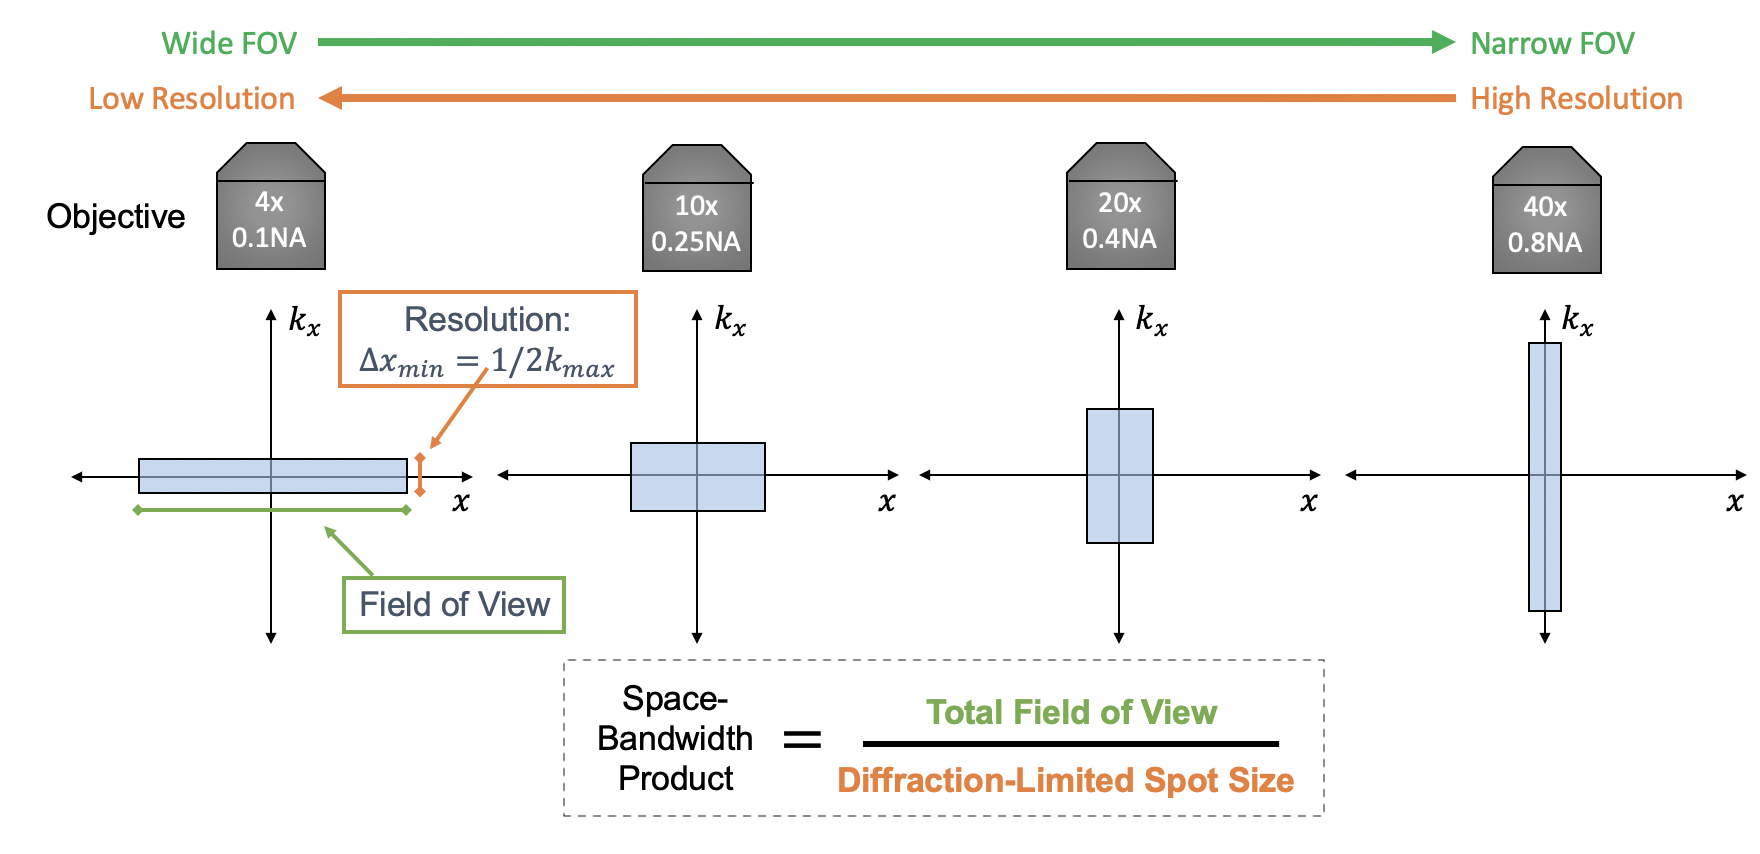
\includegraphics[width=\textwidth]{figures/fig_highthroughput_sbp.png}
  \caption{\label{fig:highthroughput_sbp} Illustration of ideal space-bandwidth product allocation for various common objective lenses as plotted in the WDF. While the area of each rectangle remains constant, the aspect ratio illustrates the allocation of bandwidth between high-resolution and a wide FOV.}
\end{figure*}

The illustration in Fig.~\ref{fig:highthroughput_sbp} reveals the regions which are most amenable to scanning for common objective types. For example, when using an objective with a high magnification and NA, it would be more optimal to scan a sample in the real domain, since each measurement will already have significant spectral coverage (resolution). Conversely, low-magnification optics are more amenable to scanning in the frequency domain to build resolution, since these systems already have a very large FOV. This intuition explains the practical benefits of performing Fourier ptychography using a low-magnification objective~\cite{Zheng2013}, since scanning is performed in the frequency domain - there would be little practical benefit to performing Fourier ptychography using a high-magnification objective and the maximum illumination NA would be roughly the same as the imaging NA (making any resolution improvement marginal compared to brightfield or DPC phase imaging).

On the other hand, mechanical scanning provides a means for augmenting the SBP in real-space, making it amenable for high-magnification imaging systems. A basic example of this technique is slide-scanning systems, which move a sample while serially capturing images between each movement. A second example is conventional ptychography~\cite{rodenburg2004phase}, which probes a sample in real-space while imaging the diffracted field in the Fourier domain (usually using propagation onto a detector array). The choice of which scanning method to use is a general question and is beyond the scope of this work, but would certainly depend on the relative acquisition bottlenecks present in each system, and would be best compared using the SBR. Figure~\ref{fig:highthroughput_scanning} illustrates these two scanning techniques.

\begin{figure*}
  \centering
    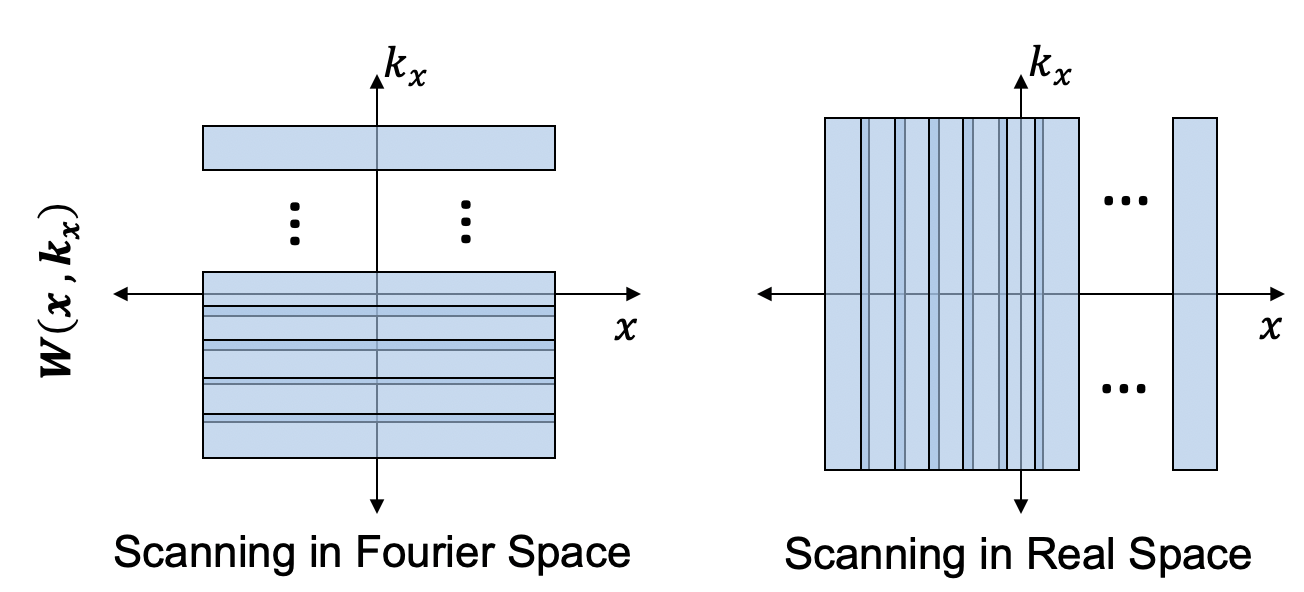
\includegraphics[width=\textwidth]{figures/fig_highthroughput_scanning.png}
  \caption{\label{fig:highthroughput_scanning} Comparison of spectral and spatial scanning techniques in high-throughput systems.}
\end{figure*}

A final parameter of interest is the signal-to-noise ratio (SNR) of the recovered images. In imaging, SNR is generally defined as ratio of the mean signal to the standard deviation of the background (As described in Eq.~\ref{eq:intro_snr}). The absolute SNR requirements vary based on applications; generally speaking, a $SNR > 10$ is considered a threshold where images have good SNR, although images below this threshold are also useful for many applications. The SNR is inherently tied to space-bandwidth rate because SNR will always increase for larger exposure times, which would conversely lead to a lower SBR due to longer dwell times for each measurement. Therefore, it is important to consider a minimum SNR as an additional constraint on the speed of the optical system. Practically, this trade-off is most noticeable under strobed illumination, where a dim illumination source and short exposure time can cause low measurement SNR. Decreasing sample velocity will increase SNR, but at the cost of a slower overall acquisition. The remaining sections of this paper present a method for increasing the SNR of measurements, which could also be interpreted as increasing the maximum SBR to maintain a necessary minimum signal-to-noise ratio.

\begin{figure*}
  \centering
    \includegraphics[width=\textwidth]{figures/fig_highthroughput_system.pdf}
  \caption{\label{fig:system}High throughput imaging system with coded illumination. A.) Our system consists of an inverted optical fluorescence microscope with a 2-axis motion stage, illuminated using a programmable LED illumination source. In our proposed method, the sample is illuminated with many discrete pulses while being scanned at constant velocity. B.) Comparison between conventional high-throughput imaging techniques (stop-and-stare, strobed illumination) and our proposed coded illumination technique. Coded illumination provides a trade-off between SNR and acquisition speed, particularly for low-light situations such as fluorescence imaging. C.) Image of our system, which is a Nikon TE300 microscope configured with a Prior motion stage and LED illuminator.}

\end{figure*}

\section{High-Throughput Microscopy with Motion Deblurring}
In this section, we propose a novel computational imaging technique which employs a coded-illumination acquisition and deconvolution to meet the demands of high-throughput applications which require a minimum SNR. Our method involves illumination the sample with multiple pulses during each acquisition in order to improve the SNR compared to strobed illumination, while maintaining a high acquisition rate. With knowledge of this pulse sequence and motion trajectory, the blurred image can be used to perform a reconstruction of the static image, with higher SNR than a comparable strobed acquisition. Our method employs a motion-multiplexing technique to enhance the measurement SNR of our system by illumination with a sequence of short, bright pulses every frame. The captured images contain motion-blur artifacts, which must be removed computationally through a motion deblurring algorithm~\cite{raskar2006coded}. The overall gain in SNR is proportional to the number of pulses as well as the conditioning of the motion deblurring process~\cite{agrawal2009optimal}, necessitating careful design of pulse sequences to produce the highest-quality image. In the following sections, we detail the joint design of the hardware and algorithms to enable gigapixel-scale fluorescence imaging with improved SNR,
compare the performance of our proposed framework against traditional methods, and provide an experimental demonstration of situations where coded illumination is both optimal (e.g. fluorescence imaging) and sub-optimal (e.g. brightfield imaging) as a function of common system parameters such as illumination power and camera noise levels. Thus, our contribution is both the proposal of a new high-throughput imaging technique as well as an analysis of when it is practically useful for relevant applications.

\begin{figure}
  \centering
    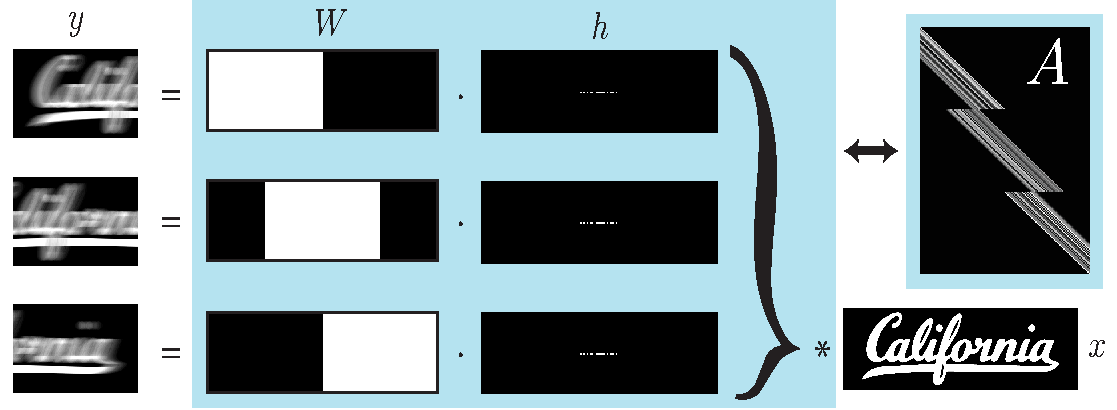
\includegraphics[width=\textwidth]{figures/fig_highthroughput_forward_model.pdf}
  \caption{\label{fig:forward_model}Multi-frame forward model. Here $[*]$ represents 2D convolution and $[\cdot]$ represents the element-wise product.}
\end{figure}

\subsection{Methods}
\subsection{Motion Blur Forward Models}
With knowledge of both sample trajectory and illumination sequence, the physical process of capturing a single measurement of a sample illuminated by a sequence of pulses while in motion can be mathematically described as a convolution:

\begin{equation}
\label{eq:single_forward}
\image = \kernel * \object + \noise,
\end{equation}

\noindent where $\image$ is the blurred measurement, $\object$ is the static object to be recovered, $\noise$ represents additive noise, $*$ represents 2D convolution, and $\kernel$ represents the blur kernel, the mapping of the temporal illumination intensity to positions in the imaging coordinate system using kinematic motion equations. With appropriate padding, this convolution can be computed efficiently using the Fourier Transform, and can be similarly inverted using FFT-based deconvolution.

To use coded illumination for large FOV imaging, we propose an extension of the single-frame forward model to the multi-frame case. 
Mathematically, we model the serial acquisition of motion-blurred frames as the vertical concatenation of many single-frame forward models, which are individually convolutional (Fig.~\ref{fig:forward_model}). 
In our model, each captured image has an associated blur operator $\B_j$ defined by each blur kernel $\h_j$ such that $\h_j * \x = \B_j \x$.
Additionally, we prepend each convolutional sub-unit with a crop operator $\W_j$, which selects an area of the object based on the field-of-view of the camera. Together, these operators encode both spatial coverage and the local blurring of each measurement, and are concatenated to form the complete multi-frame forward operator:

\begin{equation}
\label{eq:multiframe_forward}
\begin{bmatrix}\y_1\\ \vdots \\ \y_n \end{bmatrix} = \begin{bmatrix}\W_1\B_1 \\ \vdots \\ \W_n \B_n \end{bmatrix} \x + \noise = \A\x + \noise\:
\end{equation}

This forward operator $\A$ is no longer generally convolutional, taking the form of a spatially variant convolution based on the coverage of each individual $\W_j$. A one-dimensional illustration of the multi-frame smear matrix $\A$ is displayed in Fig.~\ref{fig:forward_model}. 
With the addition of appropriate windowing logic, the forward operation and its adjoint can be computed efficiently for use in iterative reconstruction.

\begin{figure*}
  \centering
    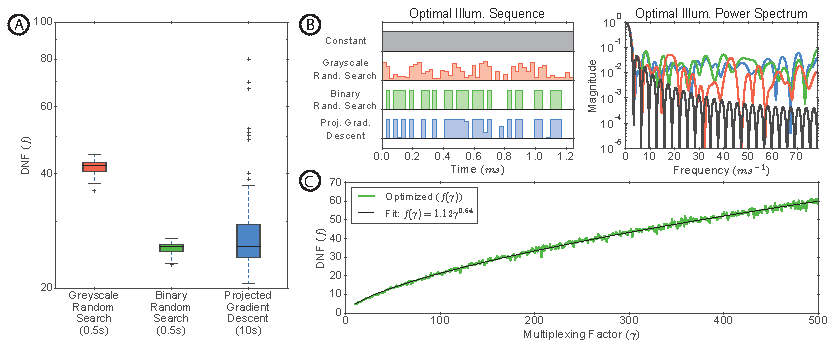
\includegraphics[width=\textwidth]{fig_highthroughput_illumination_optimization.pdf}

  \caption{ \label{fig:illum_optimization} A.) Resulting DNF values for illumination patterns generated by different optimization methods show that random search over binary patterns is of comparable effectiveness to the projected gradient descent method. B.) Example illumination sequences show differing power spectra between constant illumination and patterns generated by random search over greyscale, random search over binary, and projected gradient descent. C.) Optimized DNF (binary random search method) is plotted over different values of $\gamma$. A power law fit of $f(\gamma) = 1.12 \gamma^{0.641}$ has standard error of $1.075$.}
\end{figure*}

\subsection{Reconstruction Algorithm}\label{sec:highthroughput:recon}
To invert our forward model (\eqref{eq:multiframe_forward}), we employ Nesterov accelerated gradient descent~\cite{nesterov} algorithm to minimize the distance between our measurements $\y$ and estimated object $\widehat \x$ passed through forward model $\A$ in the $\ell_2$ metric. For the purposes of this work, we seek to minimize an unregularized cost function, $O(\x) = \frac{1}{2}\|\A\x - \y\|_2^2$ using the following update equations at each $k^{th}$ iteration:

\begin{align}\label{eq:reconstruction}
\begin{split}
    \vec z^{k+1} &= \x^k - \alpha \A^\top (\A\x - \y) \\
    \x^{k+1} &= \beta^k \vec z^k + (1-\beta^k) \vec z^{k+1}\:    
\end{split}
\end{align}
Here, $\alpha$ is a fixed step size and $\beta^k$ is set each iteration by the Nesterov update equation.

In all reconstructions we performed 30 iterations of~\eqref{eq:reconstruction}, which we found was a favorable balance of reconstruction quality and reconstruction time. While adding a regularization term such to enforce signal priors could improve reconstruction quality (and was previously analyzed in the context of motion deblurring~\cite{mitra:2014}), we chose not to incorporate regularization to provide a more fair and straightforward comparison between the proposed coded illumination acquisition and conventional strobed and stop-and-stare acquisitions. It should be noted that running our algorithm for a pre-defined number of iterations may provide some regularization from early-stopping~\cite{hagiwara2000regularization}.

Reconstructions were performed in Python using the Arrayfire GPU computation library~\cite{Yalamanchili2015}. 
Due to the structure of our scans (Figure~\ref{fig:system}A), the reconstruction algorithm is highly parallelizable -- we separate our reconstruction into strips along the major translation axis to perform 1D convolutions, and stitch these strips together after computation. 
Using this parallelization, we are able to reconstruct an approximately 1 gigapixel FOV in approximately 2 minutes. Further details of the reconstruction implementation are discussion in Section~\ref{sec:highthroughput:results}.

\subsection{Reconstruction SNR}\label{sec:highthroughput:methods_snr}

To minimize the error between the reconstructed $\widehat \x$ and the true object $\x$, the blur kernels and scanning pattern should be chosen such that the noise is minimally amplified by the inversion process. This amplification is controlled by the singular values of the forward model $\A$. 

In the case of single-frame blur, the singular values are controlled by the length and coding of the blur kernel $\h$. 
While early works~\cite{raskar2006coded, Ma:15} used a non-linear optimization routine (i.e. the \texttt{fmincon} function in MATLAB (Mathworks)) to minimize the condition number of $\A$, more recent work proposed maximizing the reconstruction signal-to-noise ratio directly, using camera noise parameters, source brightness, and the well-posedness of the deconvolution~\cite{agrawal2009optimal, cossairt2013does}. 

We extend this work to the multiframe setting.
In our analysis, we adopt the convention of imaging SNR, which is the ratio of the mean signal to the signal variance (due to photon shot noise, camera readout noise, fixed pattern noise, and other camera-dependent factors). Under a simplified model, the noise variance will be the addition in quadrature of the camera read noise variance $\sigma^2_{r}$ plus a signal dependent term $\bar{s}$:

\begin{equation}
    \label{eq:snr}
    SNR = \frac{\bar{s}}{\sqrt{\bar{s} + \sigma^2_{r}}}\;
\end{equation}

Here, we ignore exposure-dependent noise parameters such as dark current and fixed-pattern noise, since these are usually small for short exposure times relative to read noise $\sigma^2$. Note that the denominator of~\eqref{eq:snr} is equivalent to the standard deviation of $\noise$ in~\eqref{eq:single_forward}. This definition is valid for both strobed illumination and stop-and-stare acquisitions. For an acquisition performed using coded illumination, it is necessary to consider the noise amplification that results from inverting the forward model. As defined in previous work~\cite{agrawal2009optimal}, this amplification is controlled by the deconvolution noise factor (DNF), which for single-frame blurring is defined as:

\begin{equation} \label{eq:DNF}
f = \sqrt{\frac{1}{m} \sum_{i=0}^m \frac{\max_i{|\tilde{\h}|_i^2}}{|\tilde{\h}|_i^2}}\:
\end{equation}
In~\eqref{eq:DNF}, $m$ is the size of the blur kernel $\h$, and $\tilde{\h}$ represents the Fourier transform of $\h$. % Note that for a convolutional forward model, the magnitude of the Fourier coefficients of the kernel $\h$ ($|\tilde{\h}|$) are the singular values of the convolutional operator $\B$ which performs a convolution with $\h$.


\begin{figure*}
  \centering
    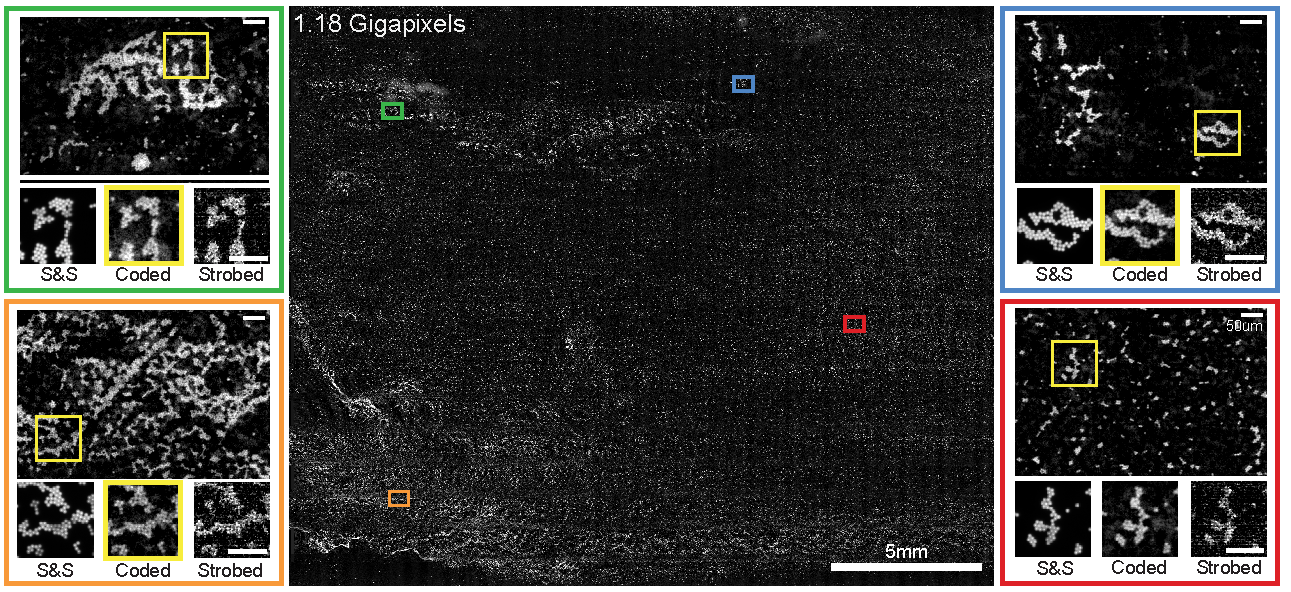
\includegraphics[width=1.0\textwidth]{fig_highthroughput_full_field.pdf}
    
  \caption{(1.18 gigapixel, 23mm $\times$ 20mm full-field reconstruction of 4.7$\mu m$ fluorescent microspheres. Inset scale bars are 50$\mu m$. While coded reconstructions have lower SNR than stop-and-stare (S\&S) measurements, measurements acquired using coded illumination (Coded) were more than 5.5$\times$ faster while maintaining enough signal to distinguish individual microspheres compared to strobed illumination (Strobed)}

\end{figure*}

To write an expression for the singe-frame SNR under coded illumination, we first define a multiplexing factor $\gamma=\sum_{i} h_i$, the total amount of illumination imparted during exposure. If $\h$ is constrained to be binary, $\gamma$ will be equal to the number of pulses in $\h$. \eqref{eq:snr} can the be modified using both $f$ and $\gamma$:

\begin{equation}
    \label{eq:snr_coded}
    SNR  = \frac{\gamma\bar{s}_0}{f\sqrt{\gamma\bar{s}_0 + \sigma^2_{r}}}\:
\end{equation}
In~\eqref{eq:snr_coded}, $\bar{s}_0$ is the mean signal imparted by a single illumination pulse. We include the complete derivation of~\eqref{eq:snr_coded} in Appendix~\ref{sec:appendix:snr_derivation} for completeness. 

The derivation of this quantity relies on the convolutional nature of single-frame motion blur. 
However, the multi-frame forward operator $\A$ has the form of a spatially variant convolution matrix. As shown in Fig.~\ref{fig:forward_model},
each column of this matrix defines a localized convolutional kernel; near the horizontal boundaries between the different frames, the vertical combinations of kernels are non-trivial. 
While methods for analyzing spatially variant convolution matrices exist~\cite{chan2011bounds}, we focus our analysis on a practical simplifying assumption: blur path and illumination patterns are fixed to be the same across all frames, i.e. $\h_j=\h$ for all $j$.

In this special case, the resulting SNR of the proposed multi-frame model is governed by both the power spectrum of the blur kernel and the spatial coverage of the crop operators. We define $c_i$ to be the \textit{coverage} at pixel $i$, i.e. the number of times pixel $i$ is included in the windows $\{\W_1,...,\W_n\}$.
The SNR for a multi-frame acquisition with coded illumination is bounded as
\begin{align*}
    SNR  \geq \sqrt{
    \min_{i} c_i}  \cdot \frac{ \gamma\bar{s}_0}{f\cdot \sqrt{\gamma\bar{s}_0 + \sigma^2_{r}}}\:
\end{align*}

Thus, the SNR improves by at least a factor of square root the minimum coverage compared with the single-frame coded illumination case in~\eqref{eq:snr_coded}. The derivation is included in Appendix~\ref{sec:appendix:multiframe_app}.

Notably, this bound decouples the spatial coverage from the spectral quality of the blur, allowing for blur kernel optimization independent of the multi-frame aspect. A good motion path ensures even spatial coverage through $c_i$ while a good illumination sequence ensures spectral coverage through traditional single-frame methods. In what follows, we focus system design on the maximization of this decoupled lower bound. 

The decision to use the same blur kernel in every frame has several practical implications as well: the micro-controller memory would be saturated when storing more than one thousand kernels and post-processing registration is much easier since all measurements have been distorted by the same blurring operator. Additionally, the fact that this reduction requires the motion to be along single motion axis is not limiting, since in practice horizontal strips are reconstructed independently to accommodate computer memory. 

\subsection{Illumination Optimization}\label{sec:highthroughput:illum_opt}
Previous work~\cite{raskar2006coded, agrawal2009optimal} showed that reconstructions performed using constant (non-coded) illumination will have very poor quality (in terms of SNR) compared to using optimized pulse sequences or a short, single pulse. Here, we explore several approaches for generating illumination pulse sequences which maximize the reconstruction SNR (\eqref{eq:snr_coded}). We first consider the problem of minimizing the DNF ($f$) with respect to $\h$:
\begin{align}
    \begin{split}
        \label{eq:illum_opt_single}
        f(\gamma) := \min_{\h}&~~ f \\
          s.t. &~~0 \leq h_i \leq 1 \; \forall \; i, \quad
          \sum_{i} h_i = \gamma \:,
    \end{split}
\end{align}

\noindent where inequality constraint on $\h$ represents the finite optical throughput of the system. 
This optimization problem is non-convex, and it resembles those used in previous work~\cite{raskar2006coded,agrawal2009optimal,Ma:15} (Our multiplexing factor $\gamma$ is related to the kernel length $N$ and throughput coefficient $\beta$ in previous work by $\gamma = N\beta$). This definition enables a layered approach to maximizing the SNR: after solving~\eqref{eq:illum_opt_single} for each multiplexing factor, it is possible to find the one which optimizes~\eqref{eq:snr_coded} in the context of camera noise parameters.

To simplify the optimization task, the positions encoded in $\h$ may be restricted a priori, e.g. to a centered horizontal line with fixed length as in Fig.~\ref{fig:forward_model}. In the following, we constrain the positions to a straight line with length $N=2\gamma$. This provides a sufficiently large sample space for kernel optimization, and is supported as optimal by analysis in~\cite{agrawal2009optimal}.

We consider several methods for solving the DNF optimization in~\eqref{eq:illum_opt_single}: random search over greyscale kernels, random search over binary kernels, and a projected gradient descent (PGD) approach. Our random search approach is simple: a fixed number of candidate kernels are randomly generated, and the one with the lowest DNF is chosen. The grayscale candidates were generated by sampling uniform random variables, while the binary were generated by sampling indices without replacement. In our PGD approach, the kernel optimization problem (\eqref{eq:illum_opt_single} is reformulated as the minimization of a smooth objective $g(\h)$ subject to convex constraints $\mathcal{S}$.  

Starting from an initial $\h_0$, the update rule includes a gradient step followed by a projection:
\begin{align*}
    \tilde \h^{k+1} &= \mathrm{Proj}_{\mathcal{S}}(\h^k - \alpha^k \nabla g(\h))\:.
\end{align*} 
Details of the reformulation and optimization approach are presented in Appendix~\ref{sec:appendix:optimization_app}.

The box plots in Fig.~\ref{fig:illum_optimization}A show the distribution of optimization results for 100 trials of each approach, where the random search methods sample 1000 candidates and PGD runs with step-size determined by backtracking line search until convergence from a random binary initialization. Example illumination sequences from each method and their corresponding power spectra are displayed in Fig.~\ref{fig:illum_optimization}B.

Though the kernels with the lowest DNF were generated through PGD, binary random search results in comparable DNF values and is up to $20\times$ faster than PGD. Further, we note that a random binary search resulted in significantly lower DNF calculations than grayscale random search. A binary restriction also achieves fast illumination updates, since grayscale illumination (as in~\cite{Ma:15}) would require a pulse-width-modulation (PWM) cycle spread across multiple clock cycles.  

Plotting the DNF ($f(\gamma)$) generated through binary random search in Fig.~\ref{fig:illum_optimization}C reveals a concave curve. Fitting the curve with a power-law, a closed-form approximation for the DNF as is $f(\gamma)=1.12\gamma^{0.64}$. This analytic relationship allows for a direct optimization of SNR: substituting any $f(\gamma) \propto \gamma^p$ into~\eqref{eq:snr_coded} and differentiating with respect to $\gamma$, we can determine the approximately optimal multiplexing factor $\gamma^*$ as a function of mean strobed signal $\bar{s}_0$ and camera readout noise $\sigma_r^2$:

\begin{equation}
    \label{eq:optimal_gamma}
    \gamma^* = \frac{2-2p}{2p-1} \cdot \frac{\sigma_r^2}{\bar{s}_0}\:.
    % \frac{2.57143 \cdot \sigma_r^2}{\bar{s}_0}
\end{equation}

We note that for smaller $p$, i.e. slower DNF growth with $\gamma$, the optimal multiplexing factor will be larger. 
With $p=0.5$, the expression for SNR in~\eqref{eq:snr_coded} only increases with increasing multiplexing factors, meaning that the optimal $\gamma^*$ would be as large as possible given hardware constraints. 
We show in Appendix~\ref{sec:appendix:dnf_limit} the lower bound $f(\gamma)\geq \gamma^{0.5}$ regardless of optimization method or illumination sequence.
The experimental $p=0.64$ accurately reflects the practical relationship, given that we experience limitations from imperfect optimization methods. Part of the observed relationship may come from the the increasing difficultly of optimization as the decision space grows with $\gamma$. 

The expression for optimal $\gamma^*$ also solidifies the intuition that a higher multiplexing should be used for systems with high noise in order to increase detection SNR, while a lower multiplexing is appropriate for less noisy systems. This result is in agreement with~\cite{agrawal2009optimal}, in which it was demonstrated that the choice of multiplexing factor depends on the relative magnitude of the acquisition noise. 

\subsection{System Hardware and Software} \label{sec:highthroughput:hardware}
Our system is built around a inverted microscope (TE300 Nikon) using a lateral motion stage (Prior, H117). Images were acquired using a SCMOS camera (PCO.edge 5.5, PCO) through hardware triggering, and illumination was provided by a high-power LED (M470L3, Thorlabs) which was controlled by a micro-controller (Teensy 3.2, PJRC). Brightfield measurements were illuminated using one of two sources: a custom LED illuminator with 40 blue-phosphor LEDs (VAOL-3LWY4, VCC), or a single, high-power LED source (Thorlabs M470L3), both modulated using a simple single-transistor circuit through the same micro-controller. The first illuminator was designed to have a broad spectrum for brightield imaging, while the second was intended for fluorescence imaging, having a narrow spectral bandwidth. For this project, we found it was necessary to adopt very simple LED circuitry to avoid electronic speed limitations associated with dimming (PWM) and serial control of LED driver chips. A schematic and layout of our system is shown in Fig.~\ref{fig:system}A and a photograph in Fig.~\ref{fig:system}C.

The micro-controller firmware used in this device was developed as part of a broader open-source LED array firmware project~\cite{illuminate}. Images were captured through the python bindings of the Micro-Manager software~\cite{micromanager}, which were controlled through a Jupyter notebook~\cite{Kluyver:2016aa}, enabling fast prototyping of both acquisition and reconstruction pipelines in the same application. With the exception of our custom illumination device, everything in our optical system is commercially available in combinations commonly available at many imaging centers. Therefore, our method is amenable to most traditional optical setups, and can be implemented cheaply through the simple addition of our temporally coded light source and open-source software tools.

All acquisitions in this work were performed using a 10$\times$, 0.25NA objective, which had a depth of field of approximately 8.5 $\mu m$. Because this depth-of-field was relatively large compared to our sample, we were able to level the sample manually prior to acquisition using adjustment screws present on the motion stage to ensure the sample remained in focus across an approximately 20$mm$ movement range. For larger areas or shallower DOF, we anticipate a more sophisticated leveling technique will be necessary, such as active autofocus~\cite{nikonperfect, zeissdefinite}. In practice, the focal adjustment process required only a few minutes for our 10$\times$ objective, and was stable between samples (requiring infrequent adjustment).

\section{Results}\label{sec:highthroughput:results}
\subsection{Gigapixel Reconstruction}
To demonstrate the performance benefit of our system, we performed a 1.18 gigapixel reconstruction of a microscope slide plated with 4.7$\mu m$ polystyrene fluorescent beads (Thermo-Fisher) using the high-throughput coded illumination microscope shown in Fig.~\ref{fig:system}. Multiple images were captured at spatial offsets, enabling a reconstruction with extend field of view (FOV). Each scan pathway consisted of multiple 1D continuous scans structured in a raster-scanning pattern (Fig~\ref{fig:forward_model}{B}) to enable fast 2D scanning of the sample. For a complete comparison, we acquired stop-and-stare, strobed illumination, and coded illumination datasets serially, and performed image stitching and registration of the three datasets for a direct comparison of image quality. The total acquisition time for the coded reconstructions of this size was 31.6 seconds, while a comparable stop-and-stare acquisition required 210.9 seconds. The computation time for coded-illumination reconstructions using~\eqref{eq:reconstruction} with step-size $\alpha=0.5$ was approximately 30 minutes on a Macbook Pro (Apple) with attached RX580 external GPU (Advanced Micro-Devices), or approximately 2 minutes when parallellized across 18 EC2 p2.xlarge instances with Nvidia Titan GPUs (Amazon Web Services), excluding data transfer to and from our local machine.

\subsection{Method Comparison}\label{sec:highthroughput:method_comparison}

\begin{figure}
\centering
\includegraphics[width=\textwidth]{figures/fig_highthroughput_system.pdf}
  \caption{\label{fig:experimental_comparison}(Top) Experimental SNR values for a USAF 1951 resolution illuminated across a range of illumination values under strobed (square) and coded illumination (diamond). Solid lines illustrate predicted SNR based on known system parameters. Experimental SNR values are the average of 3 SNR measurements performed across the field. Green and orange data points represent inset data for fluorescent beads and resolution targets respectively. Characteristic illuminance values for LED sources, Halogen-Tungsten Lamps (Hal.), Mercury Lamps (Hg), Xenon Lamps (Xe), and Metal-Halide Lamps (M-H) are shown for reference. (Bottom) Selection of measurements used to generate the above plot. Scale bar is 25 $\mu m$.}

\end{figure}

To provide a complete comparison of our coded illumination method with existing high-throughput imaging techniques, we sought to quantify the expected SNR for each method based on relevant system parameters such as source illuminance, camera noise parameters, and desired acquisition frame-rate. In conventional high-throughput imaging it is well-understood that stop-and-stare strategy will provide higher SNR than imaging using strobed illumination, but is only feasible for low-frame rates due to mechanical limitations of the motion stage. 
%While our coded illumination method can be thought of as an improvement of strobed illumination, it will nearly always be sub-optimal compared to stop-and-stare illumination at low-frame rates due to extended exposure times without additional deconvolution noise. 
Therefore, at high frame-rates we restrict our comparison to strobed illumination and coded illumination. Later, we perform a comprehensive analysis of these trade-offs; Fig.~\ref{fig:component_analysis}A provides a visual representation of where stop-and-stare is possible in terms of mechanical parameters of the motion stage.

Using the experimental setup described in Fig~\ref{fig:system} we compare acquisitions performed under brightfield and fluorescence configurations while sweeping the output power of the LED source. In each case, we measured the illuminance at the camera plane using an optical power meter (Thorlabs). For each image and reconstruction we computed the average imaging SNR across three different regions of interest to produce an experimental estimate of the overall imaging SNR of the scene. To ensure a fair comparison, we performed no prepossessing on the data except for subtracting a known, constant offset from each measurement which was characterized before acquisitions were performed and verified with the camera datasheet. Reconstructions of measurements made using coded illumination were performed using the reconstruction algorithm described in Section 2\ref{sec:highthroughput:recon}. 

Fig.~\ref{fig:experimental_comparison} shows that coded illumination can provide up to $10\times$ higher SNR in low-illumination situations, which are most relevant for fluorescence microscopy (illuminance < 1000 lux). For brightfield microscopy, strobed illumination provides a higher SNR without additional computational complexity associated with our coded illumination method. The solid lines in Fig.~\ref{fig:experimental_comparison} are theoretical predictions of reconstruction SNR for each method based on our system parameters, which are generally in agreement with our experimental data. The methods for computing these curves are described in the following section.

\subsection{Component Analysis}\label{sec:highthroughput:component_analysis}

\begin{figure*}
  \centering
    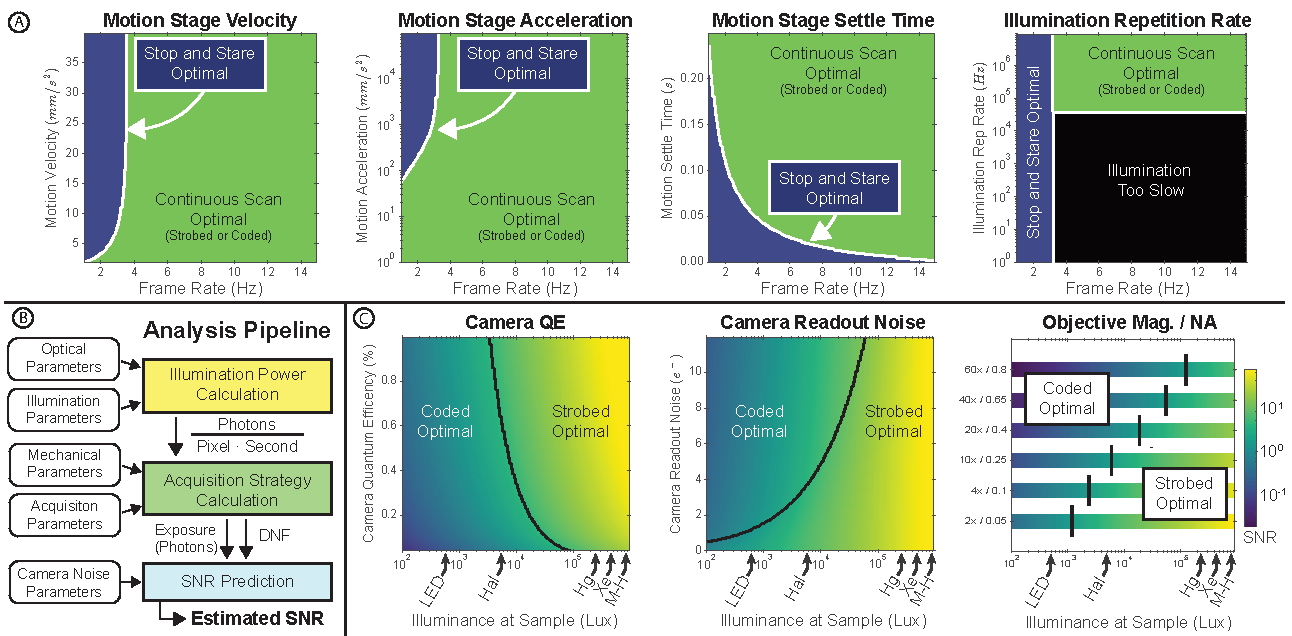
\includegraphics[width=1.0\textwidth]{figures/fig_highthroughput_component_analysis.pdf}
      \caption{\label{fig:component_analysis} Limiting Analysis of Imaging System. A.) Analysis pipeline for predicting SNR from system parameters, including illumination power, mechanical parameters of the motion stage, and camera noise parameters. B.) The stop-and-stare acquisition strategy is only possible for some configurations of mechanical system parameters and frame rates. C.) Different combinations of optical system parameters and system illuminance determine the best possible SNR and whether strobed or coded illumination is preferable. Characteristic illuminance values for LED sources, Halogen-Tungsten Lamps (Hal), Mercury Lamps (Hg), Xenon Lamp (Xe), and Metal-Halide Lamps (M-H) are shown for reference. }
\end{figure*}

In Section~\ref{sec:highthroughput:method_comparison}, we showed that the choice to use strobed or coded illumination depends heavily on the illumination power of the source; however, other system parameters may also affect this trade-off. In this section, we consider other parameters such as camera noise and motion velocity, and include an analysis of when stop-and-stare should be used as opposed to continuous-scan methods (strobed illumination and coded illumination). As a first step, we derive the expected photons per pixel, per second ($J$) we expect to measure in a transmission microscope, incorporating system magnification ($M$), numerical aperture ($NA$), camera pixel size ($\Delta$), mean wavelength ($\bar{\lambda}$, and the photometric look-up table $K(\bar{\lambda})$:

\begin{equation}
\label{eq:photonflux}
J = K(\bar{\lambda}) \bar{\lambda}\hbar c \cdot I_{lux} * (NA)^2 * (\frac{\Delta}{M})^2
\end{equation}

Here, $\hbar$ is Planck's constant, $c$ is the speed of light, $I_{lux}$ is the source illuminance in lux, and $J$ is the photon flux per pixel-second. Given $J$, the mean signal $\bar{s}$ is a function of the illumination time $t_{illum}$ and the camera quantum efficiency $Q$:

\begin{equation}
\label{eq:illuminance_to_signal}
    \bar{s} = J Q t_{illum}
\end{equation}

Substituting~\eqref{eq:illuminance_to_signal} into~\eqref{eq:snr_coded}, we can define the expected SNR as a function of these parameters as well as the blur kernel $h$ and camera readout noise $\sigma_r$:

\begin{equation}
\label{eq:photonflux_snr}
SNR = \frac{J Q t_{illum}}{f \sqrt{J Q t_{illum} + \sigma_r^2}}
\end{equation}
\eqref{eq:photonflux_snr} is used in the analysis of Fig.~\ref{fig:experimental_comparison} and Fig.~\ref{fig:component_analysis}.

The parameters $t_{illum}$ and $f$ are functions which change based on acquisition strategy. 
For stop-and-stare and strobed acquisitions, we set $f = 1$, since no deconvolution is being performed, while for coded acquisitions $f$ depends on the parameter $\gamma$ as derived in Section 2\ref{sec:highthroughput:illum_opt}. 
Similarly, $t_{illum}$ is set based on acquisition strategy and motion stage parameters. For stop-and-stare illumination, $t_{illum}$ is proportional to the residual time after stage movement, including stage acceleration ($v_{stage}$), the field of view of a single frame along the blur axis ($FOV$), mechanical settle time ($t_{stage}$), and desired acquisition frame rate $r_{frame}$:

\begin{equation}
\label{eq:sns_illum}
t_{illum} = \frac{1}{r_{frame}} - 2\frac{v_{stage}}{a_{stage}} - \frac{FOV - 0.5 * \frac{v_{stage}^2}{a_{stage}}}{v_{stage}}\:.
\end{equation}

For strobed and coded illumination, the minimum pulse duration $t_{illum}$ is set by the overlap fraction ($O$) between frames, the number of pixels along the blur direction, $N_{px}$, and the multiplexing by $\gamma$ (with strobed encoded by $\gamma=1$):

\begin{equation}
\label{eq:strobed_coded_illum}
t_{illum} = \frac{\gamma}{r_{frame}(1 - O) N_{px}}\:.
\end{equation}
In~\eqref{eq:strobed_coded_illum}, we implicitly calculate the velocity as the fastest speed where two frames may overlap with $O$ within a time set by $r_{frame}$.

Derivations for the above relationships are provided in Appendix~\ref{sec:appendix:app_throughput}. With these theoretical solutions for $t_{illum}$, we are able to derive closed-form solutions for expected SNR as a function of acquisition rate with knowledge of our system parameters (Listed in Appendix~\ref{sec:appendix:sys_param}), using the pipeline shown in Fig.~\ref{fig:component_analysis}B.

Our system analysis is divided into two parts; When stop-and-stare is possible given a desired acquisition frame rate, it will always provide higher SNR than strobed or coded illumination due to high photon counts compared to strobed illumination and no deconvolution noise. Fig.~\ref{fig:component_analysis}A analyzes where stop-and-stare is both possible and optimal compared to a continuous acquisition technique as a function of frame rate. If acquisition frame rate is low or limited by other factors (such as sample stability), stop-and-stare will always be optimal in terms of SNR. If a high-frame rate is desired, however, a continuous acquisition strategy is optimal, so long as the illumination repetition rate of the source is fast enough to accommodate sample velocity.

Fig.~\ref{fig:component_analysis}C describes the optimal continuous imaging technique as a function of illuminance, imaging objectives, camera readout noise ($\sigma_r$, and camera quantum efficiency ($QE$). Generally speaking, higher illuminance values favor strobed illumination (being shot-noise limited), while lower illuminance values favor coded illumination (being read-noise limited). Conversely, as read noise ($\sigma_r$) increases or camera $QE$ decreases, coded illumination becomes more beneficial. Practically, a camera with high read-noise with a low $QE$ will favor coded illumination more strongly (at higher source illuminance) than a high-end camera (such as the PCO.edge 5.5 used in this study), where $\sigma_r \approx 3.7 e^-$ and $QE \approx 0.6$). In addition, objectives with a higher magnification and NA will generally favor coded illumination more strongly due to the decreasing $\frac{NA}{Mag}$ ratio, although this is not necessarily true for all NA/magnification combinations due to differing optical designs. It should be noted, however, that higher NA values will require more sophisticated autofocusing methods than those presented in this work. Example illuminance values for common microscope sources were calculated based on estimated source power at 550nm~\cite{illumpower}.

\subsection{Biological Limitations}

\begin{figure}
  \centering
    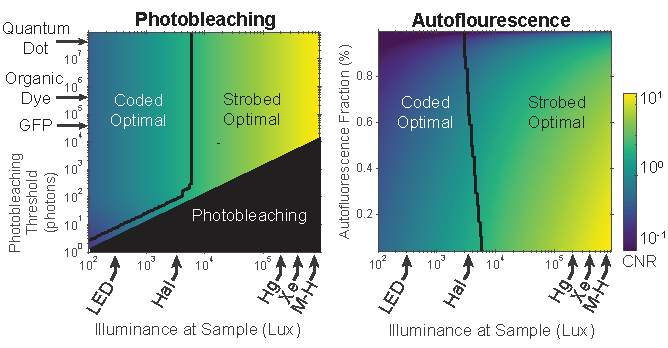
\includegraphics[width=\textwidth]{figures/fig_highthroughput_fluorescence_analysis.pdf}
      \caption{\label{fig:fluorescence_analysis} Limiting analysis of constraints imposed by the chemical fluorescence process, using contrast-to-noise ratio as the figure of merit. A.) Photobleaching influences the choice between coded and strobed illumination only when introducing a coding scheme would cause photobleaching, corresponding to a thin area of strobed optimality near the photobleaching limit. This plot assumes no background autofluorescence, so contrast-to-noise and SNR are equivalent. B.) The amount of autofluorescence relative to the signal mean has a slight effect on the optimality of strobed and coded illumination, but the effect is not strong relative to the other parameters studied here. Generally, the presence of autofluorescence degrades contrast-to-noise ratio significantly for all methods, for all illumination levels.}
\end{figure}

In fluorescence imaging, autofluorescence~\cite{autofluor} and photobleaching~\cite{lippincott2003photobleaching} are primary considerations when assessing system throughput. Photobleaching, the result of chemical interactions of activated fluorophores with the surrounding medium, is of particular concern for motion deblurring applications due to higher captured SNR compared to strobed acquisitions. Practically, photobleaching can limit the maximum number of pulses which a sample may tolerate before exhibiting a non-linear response, causing strobed illumination to become a more favorable option, even at low-light. However, the region where this condition occurs is small (for the proposed system), and near the photobleaching limit (Fig.~\ref{fig:fluorescence_analysis}A). Autofluorescence is also a well-studied process which can further degrade the quality of fluorescence images. Autofluorescence affects contrast, which is best quantified using the contrast-to-noise ratio:

\begin{equation}
    \label{eq:cnr}
    CNR  = \frac{\gamma\bar{s}_0 - \bar{b}}{f\sqrt{\gamma\bar{s}_0 + \bar{b} + \sigma^2_{r}}}\:
\end{equation}

\noindent where $\bar{b}$ is the mean background signal (autofluorescence) and all other variables are the same as in~\eqref{eq:snr_coded}. Note that in the absence of a background ($\bar{b} = 0$), $CNR$ is equivalent to $SNR$. Fig.~\ref{fig:fluorescence_analysis}B illustrates the relative optimality of strobed and coded illumination in the presence of background autofluorescence, as expressed as a fraction of the primary signal.

While significant, the lifetime of various fluorophores is not limiting at illumination speeds presented in this work. Most endogenous fluorophores and fluorescent proteins have a lifetime of less than 10$ns$, while organic dyes may have lifetimes of less than 100$ns$~\cite{fluorlifetime2010}. The fastest illumination source used in this work had a repetition period of approximately 4$\mu s$, which is 40$\times$ faster than fluorophore-limited update rate for organic dyes. Still, for future systems using motion stages moving at high velocities (such as $>100\frac{mm}{s}$ and high magnifications (greater than $40\times$), it will become more important to consider the lifetime of the dyes used. These same constraints would also apply to strobed imaging, but not stop-and-stare imaging (which does not require high-speed signal modulation).



\section{Summary}
In this chapter, we have demonstrated a novel high-throughput imaging framework which employs multi-frame motion deblurring using coded illumination. Through both experiment and theoretical analysis we have shown the applicability of out method for fluorescence microscopy, and performed a comprehensive analysis of when our method makes sense in terms of source power and other system parameters. These results indicate that coded illumination provides up to $10\times$ higher SNR than conventional strobed illumination methods in low-light situations, making our method particularly well-suited for applications in drug-discovery and whole-slide imaging. Our analysis of optimal kernel selection indicates that efficient illumination sequences can be calculated quickly and cheaply using a simple random search, and our analysis of optimal pulse length provides an approximate relationship between the length of a pulse sequence and source illuminance. Further, our proposed multi-frame reconstruction algorithm produces good results using simple accelerated gradient descent with no regularization, and can be scaled to multiple cloud instances for fast data processing. Future work should address improvements such as regularization, more complicated motion pathways, self-calibration, and reconstructions using under-sampled data.
\chapter{Fabrication of Coded Illumination Devices}

In this chapter, we explore the various illumination source types and designs for optical microscopes. Illumination sources vary significantly between microscope setups based on applications, capabilities, availability, and cost. Early microscope sources involved using a candle or oil lamp source for illumination. As early as 1665, Hooke used an oil lamp and water-filled globe to focus an oil lamp onto a sample to be imaged using his early microscope~\cite{hookeMicrographica}. These methods (along with gas lamps) were used for centuries, until the carbon arc-lamp enabled electronic illumination in the late 1800s. Around this time, K\"ohler provided a more complete understanding of proper illumination collection to avoid imaging the source directly onto the sample~\cite{kohler1893neues}, which was widely adopted and continues to be used today (including this work). As new lamp sources were invented (such as the Xenon arc lamp~\cite{anderson1951xenon}, tungsten lamp~\cite{edison1880electric}, and others) they found use in microscopy under the K\"ohler configuration. 

As fluorescent microscopy and labels were developed, these sources were often spectrally filtered to produce sharp, non-overlapping emission and excitation peaks, leading to temporally coherent illumination. In addition, spatially coherent sources were used to provide phase contrast \cite{smithDIC, zernike1942phase}, often by filtering spatially incoherent lamps using a pinhole aperture. With the invention of the laser~\cite{schawlow1958infrared}, spatially coherent illumination could be directly used, although these have had limited use as commercial microscope sources outside of fluorescence imaging due to coherent background artifacts.

In addition to illumination sources, collection optics play a major role in defining the resolution and light throughput in a microscope. In bright-field imaging, the resolution of a microscope is set by the sum of the illumination and detection (objective) numerical apertures, subject to $NA_{illumination} \leq NA_{objective}$. Illumination beyond $NA_{objective}$ is considered dark-field illumination, which can be used to reveal the locations of high-resolution features and sharp edges (without directly increasing the resolving power of the microscope). However, providing high-angle illumination ($NA_{illumination} >\approx 0.6$) in the K\"ohler configuration often requires large optics (with either short focal length or vary large diameters), which are cumbersome and expensive in most optical systems.

Illumination using light-emitting diodes (LEDs) has gradually emerged as an energy-efficient and low-cost alternative to lamp-based sources. As more diverse and efficient semiconductor materials have been discovered, LED light sources have found greater usage for both fluorescence and bright-field imaging. In addition, arrays of LEDs have been used to achieve even greater light throughput~\cite{albeanu2008led}, improve sectioning in confocal microscopy~\cite{poher2007optical}, and provide brightfield and darkfield contrast as well as 3D digital refocusing~\cite{Zheng2011}. When paired with computation, LED arrays have found significant usage for quantitative phase imaging~\cite{tian2015quantitative, phillips2015multi, chen2018quantitative}, super-resolution imaging~\cite{Zheng2013, Tian2014}, and high-throughput imaging~\cite{Ma:15}. These devices have found widespread usage within the research community due to their low-cost, simple implementation, fast switching, and relatively high light output. However, conventional LED arrays suffer from low light-throughput at high angles due to the angular emission profile of the sources and the large distances between the LED and sample.

In this chapter, we detail the design process and manufacture of several LED array designs, and discuss their performance in relevant use-cases and applications.

\section{Domed Illumination Devices for Coded Illumination}

Designing the ideal LED array source for optical microscopy is challenging, both in designing the device to compliment as many applications as possible while also being cheap to fabricate (in terms of time and monetary cost). As shown in Fig.~\ref{fig:dome_overview}, many iterations of domed LED arrays were required to construct our current prototype. As shown in~\cite{phillips2015multi, Dominguez:14}, a domed illuminator provides significantly higher intensity at high-NA, as compared to a planar array. This is due to a combination of emission profiles, field vignetting by the objective window, and reduced distance from the illuminator to the sample. For a planar array, intensity at the sample $I$ can be related to the angle of illumination $\theta$ of the emitter by the equation:

\begin{equation}
    I_{\theta} \propto {\cos(\theta)}^4
\end{equation}

\noindent where $\theta$ is the angle between the illumination vector and the optical axis. When the LEDs are arranged in a domed shape, all factors except field vignetting by the objective window are removed, reducing the intensity falloff to:

\begin{equation}
I_{\theta} \propto {\cos(\theta)}^1
\end{equation}

\begin{figure} [ht]
\begin{center}
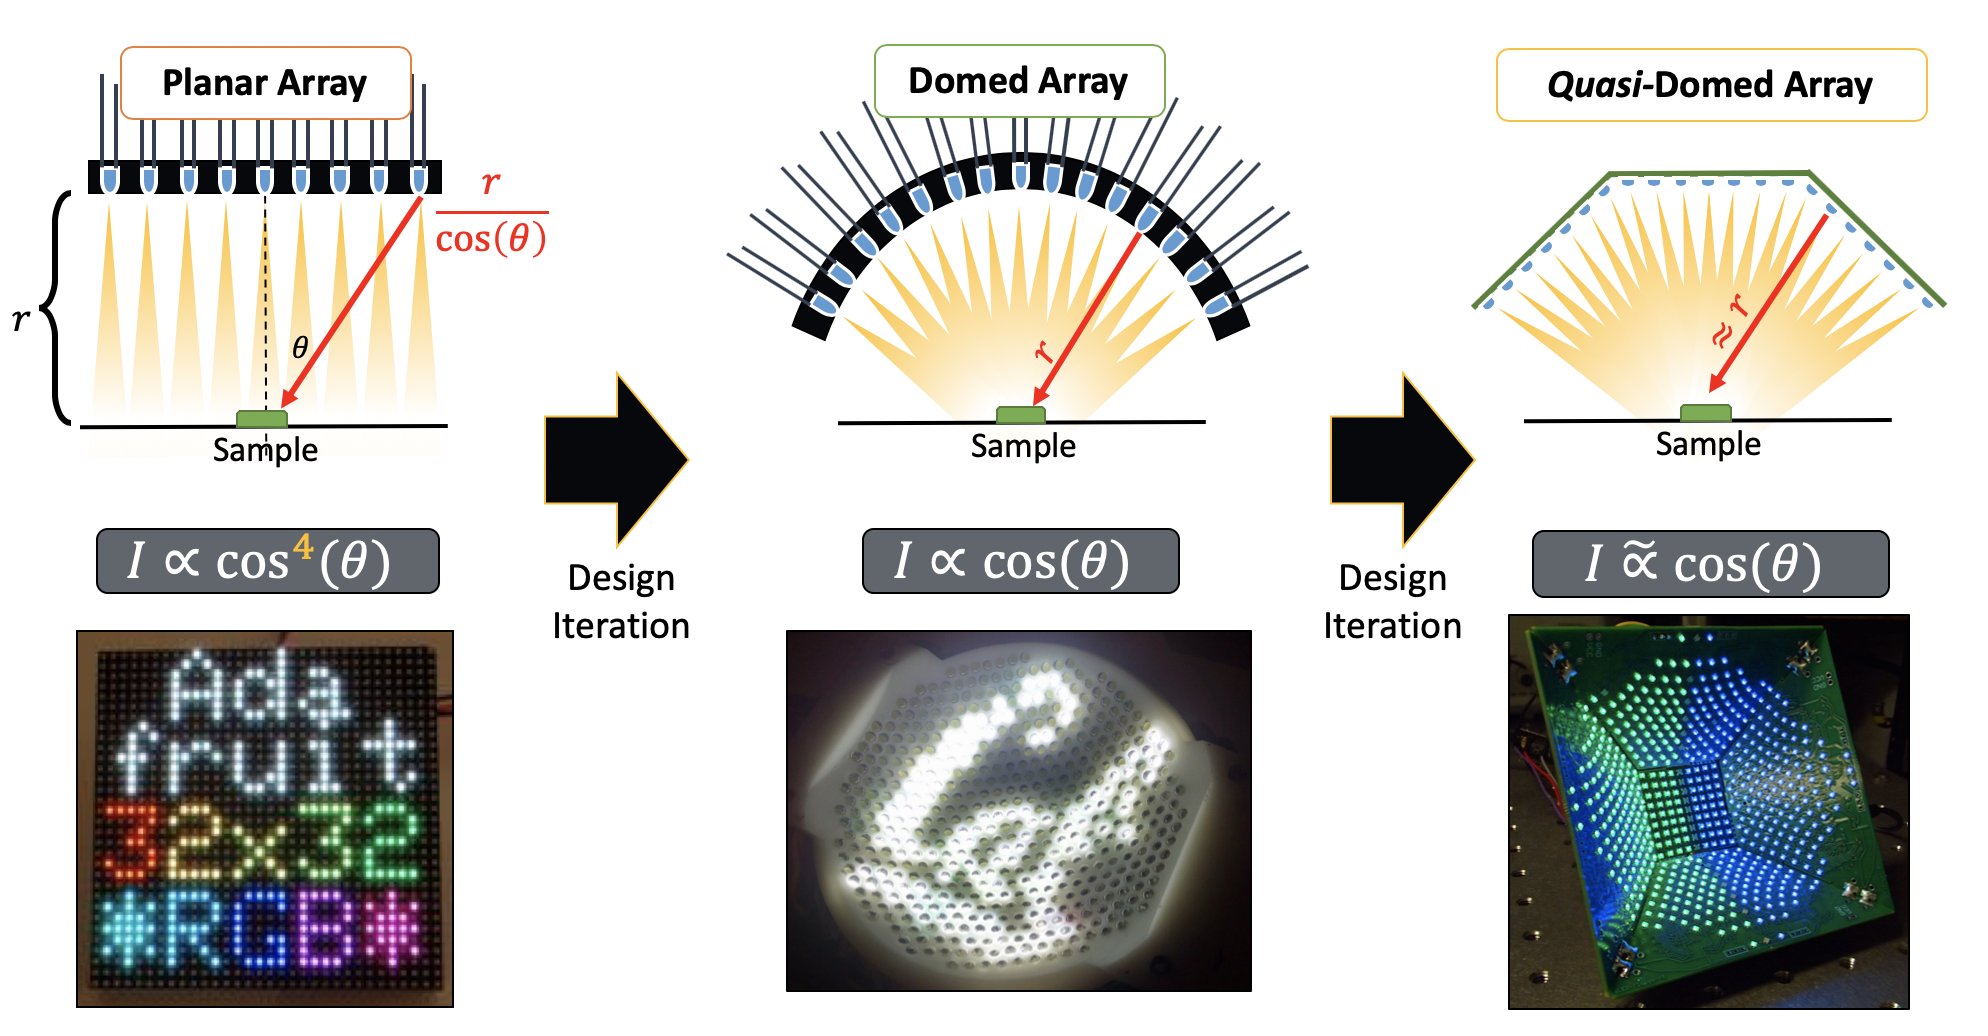
\includegraphics[width=\textwidth]{figures/fig_dome_overview.png}
\end{center}
\caption {Overview of dome designs from the Adafruit 32$\times$32 LED array to the proposed quasi-domed device. Example LED distances are provided in red.}
\label{fig:dome_overview}
\end{figure}

The illumination throughput benefits are a result of two phenomena, shown in Fig. ~\ref{fig:fabrication_ccs_dome}e. The first is that off-axis LEDs in a planar array will have a larger LED-to-sample distance and thus decreased intensity at the sample. For example, if we assume that each LED is a point emitter, the intensity falloff due to increased distance can be expressed as $I(\theta) = I_0 \cos^2(\theta)$, where $I_0$ is the intensity at the sample from the on-axis LED and $\theta$ is illumination angle. The second improvement in light efficiency comes from the fact that LEDs have significant angular variation in intensity (typically emitting more light in the forward direction). In a planar array, the LEDs at higher angles provide less effective illumination, a problem corrected by the dome geometry, where all LEDs are radially oriented. In both the domed and planar geometries we note that intensity further decreases with a final factor of $\cos(\theta)$ due to the smaller profile of objective window when viewed off-axis; combining these factors and assuming a Lambertian ($\sim\cos(\theta)$) angular dependence for physical (non-point-source) LEDs results in an expected intensity falloff of $\sim\cos^4(\theta)$ for the planar geometry but only $\sim\cos(\theta)$ for the domed geometry, a vast improvement at high incidence angles. Thus, the difference between geometries is proportional to $cos^3(\theta)$, or a factor of $> 50\%$ at $40\degree$ and $99\%$ at $77\degree$ incidence, having a substantial impact on illumination throughput, and therefore required exposure times to achieve a good SNR.

In planar arrays (such as the widely-used Adafruit $32 \times 32$ array), LEDs are conventionally uniformly spaced on the LED array. When projected onto numerical aperture (NA) coordinates, this spacing becomes tighter at high-angles, leading to an uneven sampling across the full range of illumination angles. While having a tighter spacing is usually not a problem for computational imaging applications such as differential phase contrast or Fourier ptychography, it is inefficient, and may lead to unnecessarily long acquisition times. Using a domed geometry eliminates this problem by spacing LEDs uniformly in angular, or NA coordinates. 

The minimum LED spacing depends on the application, or intended reconstruction method. In Fourier Ptychography, for example, early work~\cite{Zheng2013, Tian14, Guo:15} indicated that at least a 60\% pupil overlap was necessary in order to properly recover the complex field at high resolution. This quantity depends on the diameter of the pupil (and therefore numerical aperture of the objective); systems with smaller, low-NA objectives will have tighter requirements on LED spacing. The 60\% overlap requirement is developed to provide at least 2$\times$ overlap between measurements at every point in the Fourier domain, which is necessary to reconstruct both amplitude and phase from intensity measurements. Increased overlap beyond this requirement may provide a benefit in terms of SNR, but this effect is difficult to quantify due to the non-linear algorithm used for Fourier ptychographic reconstructions. Generally speaking, differential phase contrast has a much less stringent requirements, so long as there are 4 or more LEDs which illuminate at angles close to the objective NA.

While an LED dome is clearly necessary for obtaining high illumination intensity at high angles, practical limitations on manufacturing and assembly of non-planar circuit boards make building these domes at low cost and large scale non-trivial. In the following sections, we detail the design of a domed LED illuminator through several iterations of the design and prototyping process.

\subsection{3D-Printed Approach}\label{sec:fabrication:ccsdome}

% Dome design figure
\begin{figure} [ht]
\begin{center}
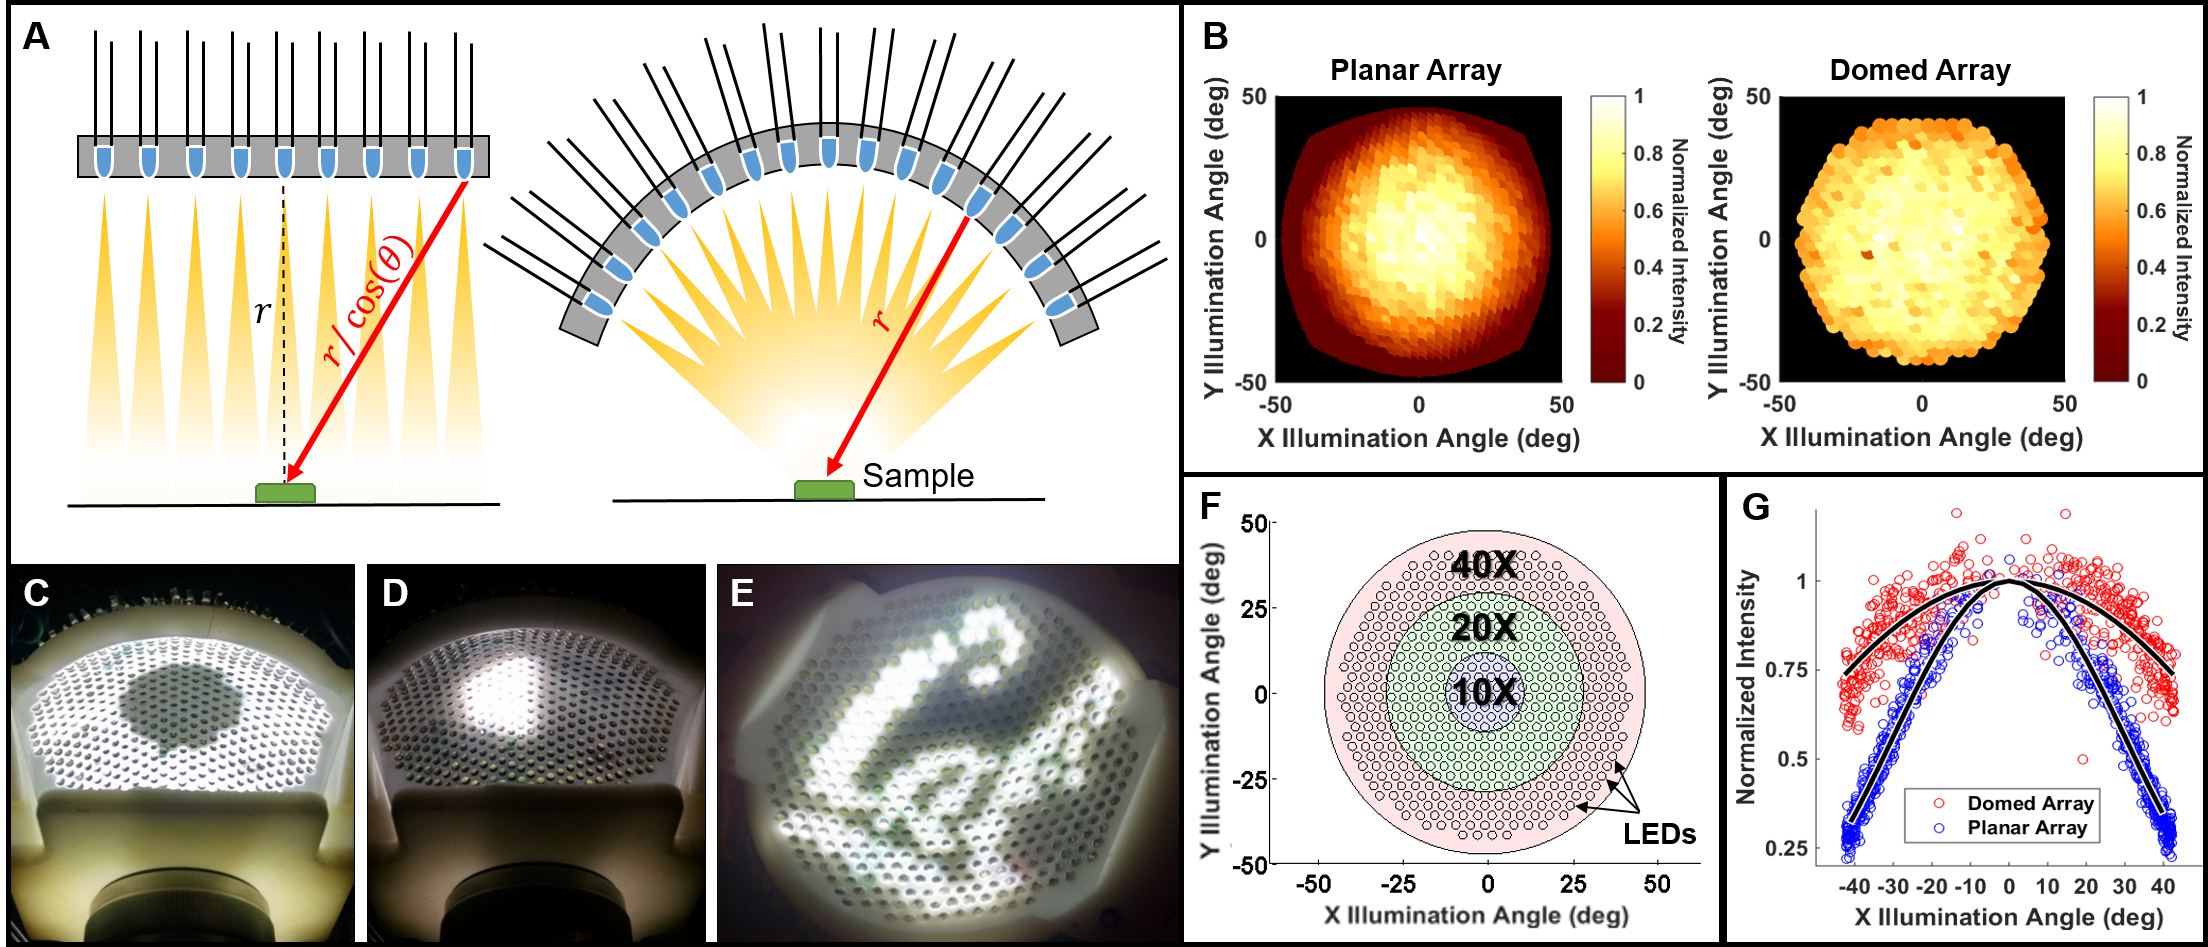
\includegraphics[width=\textwidth]{figures/fig_ccs_dome.png}
\end{center}
\caption {{ Domed LED Illuminator.}{a)} Illumination pattern used to acquire dark field images with a 0.25 NA objective.
{b)} Illumination pattern used to synthesize differential phase contrast images with a 0.25 NA objective.
{c)} Illustration of the arbitrary illumination patterning capabilities of the device.
{d)} Normalized mean pixel intensities measured at the sensor for the planar and domed arrays. Intensity decreases as a function of angle in both cases, but much more strongly in the case of the planar geometry. Values were normalized to the central LED's brightness in both cases.
{e)} Visual comparison of a planar LED array with a domed array. Since the intensity of a spherical wave drops as a function of the inverse square of radius, the illumination at the sample depends on the distance between the LEDs and the sample. In the planar case (left), LED distance $r$ increases as a function of illumination angle, causing weaker illumination at higher angles. A domed LED array (right) eliminates this variation ($r$ is constant).
{f)} Plot illustrating the relative objective NA for several common magnifications, as compared to our dome's LED placement (small black circles).
{g)} Normalized measured intensity falloff as a function of angle relative to the optical axis for the domed and planar LED arrays. Falloff is proportional to $\cos(\theta)$ for the domed geometry and $\sim\cos^4(\theta)$ for the planar geometry. Black lines are $\cos(\theta)$ and $\cos^4(\theta)$ fits for the domed and planar geometries, respectively. The domed geometry exhibits significant improvements in intensity at large angles of illumination.
}
\label{fig:fabrication_ccs_dome}
\end{figure}

The first iteration of domed illuminators was heavily inspired by the AWARE gigapixel camera series~\cite{brady2012multiscale, marks2014characterization, llull2015characterization}, where hundreds of individual cameras were manually inserted into an aluminum dome which enforced opto-mechanical constraints on directionality and position through a hexagonal camera packing. In this endeavor, we designed and fabricated a 3D-printed domed illuminator consisting of 508 individually addressable broad spectrum (white) LEDs uniformly distributed across an approximately hexagonal packing pattern across a 77 degree cone of angles corresponding to an illumination NA of 0.62. In general, the design is modular and features simple electronics, including the use of the inexpensive and widely used Arduino micro-controller platform. LED brightness control was achieved using pulse-width modulation (PWM) of the LED intensity in time using a 1MHz clock signal. The TLC5926 chips were serially connected in a daisy-chain configuration, enabling their control with a single serial connection. Pattern updates took approximatly 30ms.

The completed prototype is shown in Fig.~\ref{fig:fabrication_ccs_dome}. The experimentally measured angular illumination power of this dome matches well with theory (Figs.~\ref{fig:fabrication_ccs_dome}d,g), where the measured intensity is shown for both geometries out to 40˚ incidence. Variations in intensity between LEDs may also come from electrical variations such as batch differences in controller chips and resistor tolerances. Overall, this prototype was very difficult to manufacture because LEDs had to be inserted by hand, and the leads of each LED had to be manually soldered to one of the 9 circuit boards above the dome. This 3D reconstruction process required significant time and effort to ensure all of the LEDs were functional. The designs of this illuminator were published publicly, but to our knowledge there were no successful reproductions, owing to the difficult fabrication process.

\subsection{Quasi-Dome}\label{sec:fabrication:quasidome} 

\begin{figure}
    \centering
    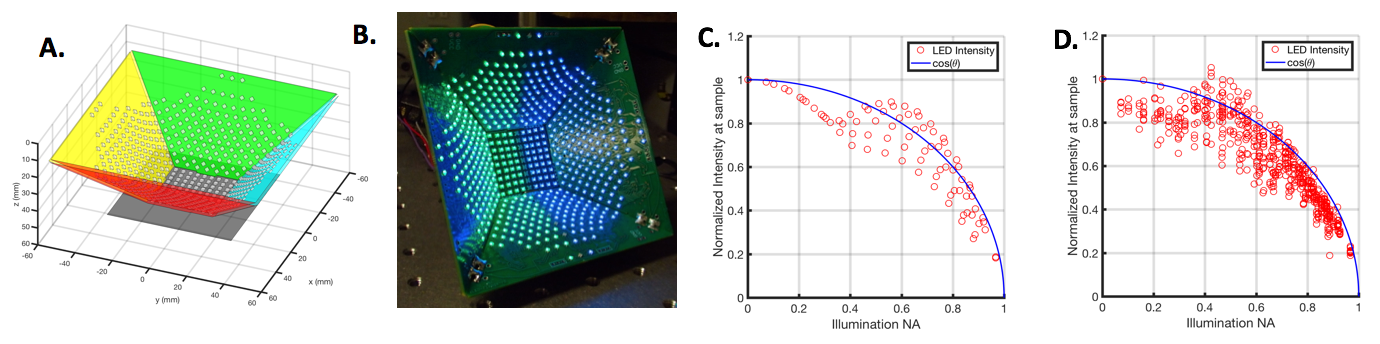
\includegraphics[width=\textwidth]{figures/fig_qdome_main.png}
    \caption{Quasi-dome programmable LED illuminator. (a) CAD model of LED flange positions. (b) Assembled LED array quasi-dome displaying two half circles (center line of LEDs are turned off). (c) Simulated intensity falloff of LED array considering all factors (normalized). (d) Experimental normalized intensity falloff.}\label{fig:fig_fabrication_quasi_dome}
\end{figure}

In response to difficulties experienced in fabricating the 3D-printed dome, we developed a quasi-domed LED array consisting of 5 panels (see Fig.~\ref{fig:fig_fabrication_quasi_dome}a,b), each of which are standard printed circuit boards with all components pre-assembled using standard printed circuit board (PCB) manufacturing techniques. Our circuit uses multi-channel LEDs (Knightbright APTF1616SEEZGQBDC) which have individual channel control without multiplexing using on-board LED Controllers (Texas Instruments TLC5955), connected in a serial daisy-chain (Fig.~\ref{fig:fabrication_dome_circuit}). This electrical configuration enables 16-bit LED intensity control of each channel (using PWM) with fast pattern updates (10ms) due to high-speed serial control via a Teensy 3.2 Microcontroller (PJRC). The software used to control this illuminator was released as the open-source illuminate LED array firmware~\cite{illuminate}.

Exact LED flange geometry was selected to provide sufficient overlap of sample spectrum areas for Fourier Ptychography. We selected 0.1 NA as our minimum objective numerical aperture, commonly corresponding to a $4\times$ objective. This spacing was used to select LED positions with even spacing in Fourier space, lending to the large LED spacings on the circuit boards at high angles. Fig~\ref{fig:fig_fabrication_quasi_dome}d shows the experimental intensity fall-off of radially projected LEDs as measured at the sensor, showing good agreement between theoretical illumination falloff due to the $\cos(\theta)$ term and experimental measurements. The use of color LEDs enabled color multiplexing, which was used to perform single-shot DPC imaging (cDPC)~\cite{PhillipsChen17cDPC}.

This quasi-domed geometry allows LED domes to be produced at scale, enabling us to fabricate 10 LED domes in the time it took to fabricate the 3D-printed design. This allowed is to use and distribute our devices to research groups around the world, including the UK, Australia, Germany, and Sweden.

\begin{figure}
    \centering
    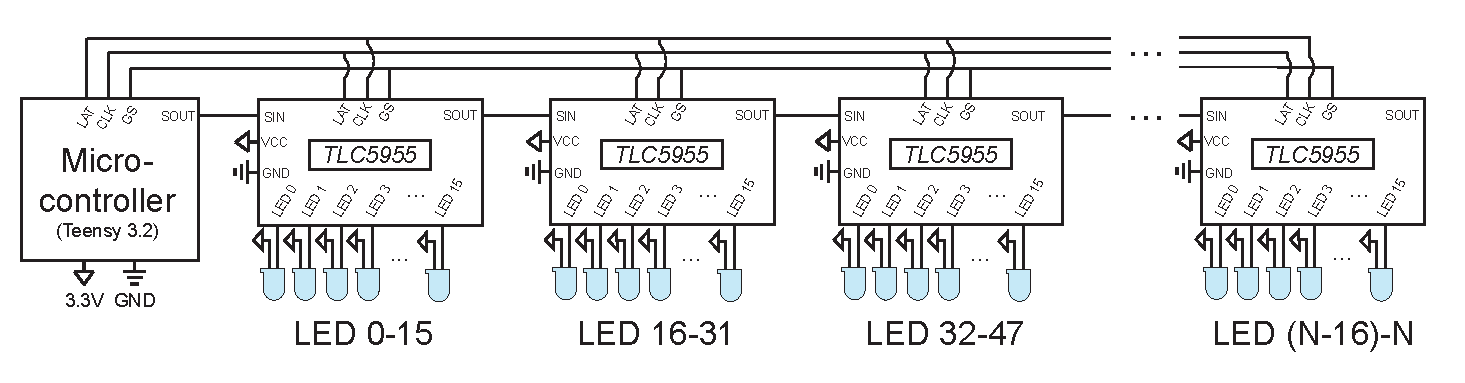
\includegraphics[width=\textwidth]{figures/fig_fabrication_slow_circuit.pdf}
    \caption{Circuit schematic for Quasi-dome device. A chain of up to 40 TLC5955 chips are connected in a daisy-chain configuration, having common Power (VCC), ground (GND), Grayscale-clock (GS), serial clock (SCLK), and latch (LAT) pins. These are controlled by a micro-controller upstream, which enables the control of up to $16 \times N_{tlc}$ LEDs for $N_{tlc}$ TLC5955 chips.}\label{fig:fabrication_dome_circuit}
\end{figure}

\subsection{Coded Illumination Devices for High-Throughput Illumination}\label{sec:fabrication:highthroughput}

High throughput imaging using both strobed illumination and motion deblurring~\cite{raskar2006coded} requires light sources to be extremely fast compared to the domed devices presented in the previous section. In these systems, the sample is imaged and illuminated while being moved continuously by a mechanical motion stage, without stopping. The key requirement of a high-throughput illumination source is repetition rate, or the minimum pulse duration the source can provide. This time must be less than the time required for the sample to move one effective pixel size (pixel size divided by magnification) while being scanned. Mathametically, the source repetition period $T$ is related to the motion velocity $v_{motion}$, camera pixel size $\Delta$, and system magnification $M$ by the following relationship:

\begin{equation}
    T \leq \frac{\Delta}{Mv_{motion}}
\end{equation}

For practical systems (such as those described in Chapter 3), this threshold is on the order of micro-seconds, which is 3-4 orders of magnitude faster than the LED domes described in previous sections. For these applications, it was necessary to adopt very simple LED circuitry to avoid electronic speed limitations associated with dimming (PWM) and serial control of LED driver chips. As such, we adopt an extremely simple circuit, consisting of only a micro-controller and transistor, to control an arbitrary number of LED sources at very high speed, limited only by the clock-speed of the microcontroller. The drawback of this configuration is that only binary illumination is possible, but binary illumination is often optimal for both strobed and coded illumination (See Chapter 3).

For these applications, we developed two sources based on the same platform, one for high-throughput brightfield and quantitative phase imaging, and one for fluorescence imaging. The first device used 40 white (blue-phosphor) LED emitters (VAOL-3LWY4, VCC) controlled by four transistor circuits to modulate 4 quadrants of a circle. The intention of this design was to enable extremely fast brightfield and quantitative phase imaging, where the sample may be color or spectral filtering could be provided downstream in the optical system. The second used a single, high-power LED source (Thorlabs M470L3) modulated using a simple single-transistor circuit through the same micro-controller. Chromatic filters could be added to the illuminaiton pathway and detection pathway to enable fluorescence imaging, and this device was compatible with a wide range of LED sources due to it's modular design. Both of these devices used the same firmware as The micro-controller firmware, which was designed to be modular to accommodate various LED arrays~\cite{illuminate}. A schematic of this high-speed circuit is shown in Fig.~\ref{fig:fabrication_highthroughput_circuit}.

\begin{figure}
    \centering
    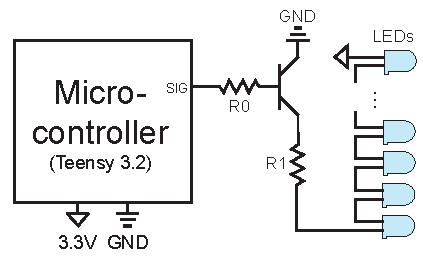
\includegraphics[width=0.5\textwidth]{figures/fig_fabrication_fast_circuit.pdf}
    \caption{Circuit schematic for fast LED driver circuit. A transistor (NPN type) is used to modulate a large current source for controlling many LEDs at once, which are connected in serial. Resistors R0 is normally set to 1K$\Omega$, and R1 is set such that the current is not too large based on the VCC voltage. This circuit enables micro-controller limited illumination updates, although it does not allow per-channel dimming and supports only binary illumination patterns.}\label{fig:fabrication_highthroughput_circuit}
\end{figure}

\section{Coded Illumination Devices for Portable Microscopy}
Optical microscopy is an important tool for disease screening and diagnosis throughout the world. Significant resources have been devoted to developing portable and affordable compact microscopes for remote clinical applications~\cite{Zhu2011, switz2014low, smith2011cell, maamari2013mobile,C4LC00010B,Vashist2014, steenblik2005lenses, cybulski2014foldscope, boppart2014point, Greenbaum17122014, mudanyali2010compact, tseng2010lensfree}. 
Compact microscopes based on mobile phones, including CellScope~\cite{breslauer2009mobile, skandarajah2014quantitative}, have demonstrated that microscopy can be effectively performed outside of hospitals and diagnostic laboratories by minimally trained healthcare workers, that images can be transmitted for confirmation of diagnosis, and that phone-based computational analysis can be used to provide automated diagnosis.

\subsection{Computational CellScope}\label{sec:fabrication:ccs}
Here, a new variation of the CellScope microscope is demonstrated which incorporates recently developed techniques of computational illumination~\cite{Zheng2011, Tian14, zijiMulti} to enable new imaging modalities, including darkfield, phase imaging and digital refocusing\footnote{This work was developed in close collaboration with Daniel Fletcher, Mike D'Ambrosio, and Neil Switz (Fletcher Lab, Bioengineering, UC Berkeley), as well as Lei Tian, Jared Rulison, Hurshal Patel, Nitin Sadras and Aditya Gande (Waller Lab, EECS, UC Berkeley).}. Using the same LED array illumination, Computational CellScope also implements lightfield digital refocusing, so that a sample focus can be changed after the fact (without mechanically changing focus) and 3D image stacks can be extracted for both intensity and phase modes. Further, constant focus correction (auto-focusing) can be implemented in post-processing for long time-lapse studies. The digital refocusing is achieved by sequentially illuminating the sample from each of the LEDs that lie inside the numerical aperture (NA) of the objective, then post-processing to form a stack of through-focus images of intensity~\cite{Ng2005,Zheng2011} or phase contrast~\cite{Tian14}. For thick samples, the result also provides a 3D reconstruction of the sample, similar to limited angle tomography.

The computational illumination techniques used here have been previously demonstrated in a traditional microscope using a planar LED array ~\cite{Zheng2011,Zheng2013,Tian14,zijiMulti,tian20153d}. The purpose of the LED array is to flexibly pattern illumination angles at the sample by turning on different sets of LEDs corresponding to different illumination angles. The optimal arrangement of LEDs, however, is not planar but rather a dome shape ~\cite{Dominguez:14}, which we utilize here. The domed arrangement provides significant improvements in intensity uniformity and light throughput, since LEDs can be directionally biased and arranged at uniform radius from the sample. These benefits contribute to increased signal-to-noise ratio (SNR) in the darkfield images, allowing effective high angle illumination patterning and shorter exposure times.

The flexibility and speed of the programmable LED array illuminator, as well as the lack of moving parts and low cost, make the hardware very amenable to modification as a CellScope attachment. In order for our device to be practically useful in the field, we have here enforced the requirement that all of our processing and control be performed on the smartphone, without use of a PC. Thus, the device can be field-deployable as a simple add-on to CellScope. In the following sections we detail the design and performance of the hardware and software of our new Computational CellScope device.

While our addition involves custom LED drive circuitry and a 3D printed structure, complexity was kept low to preserve the low-cost nature of CellScope. Part counts, cost and especially size may be further reduced in design-for-manufacture. The size of the illuminator could be reduced to essentially the dimensions of the dome itself, and cost could be comparable to the price of a modern smartphone, matching and improving upon the functionality of a full-size microscope at a fraction of the cost.

\begin{figure} [ht]
\begin{center}
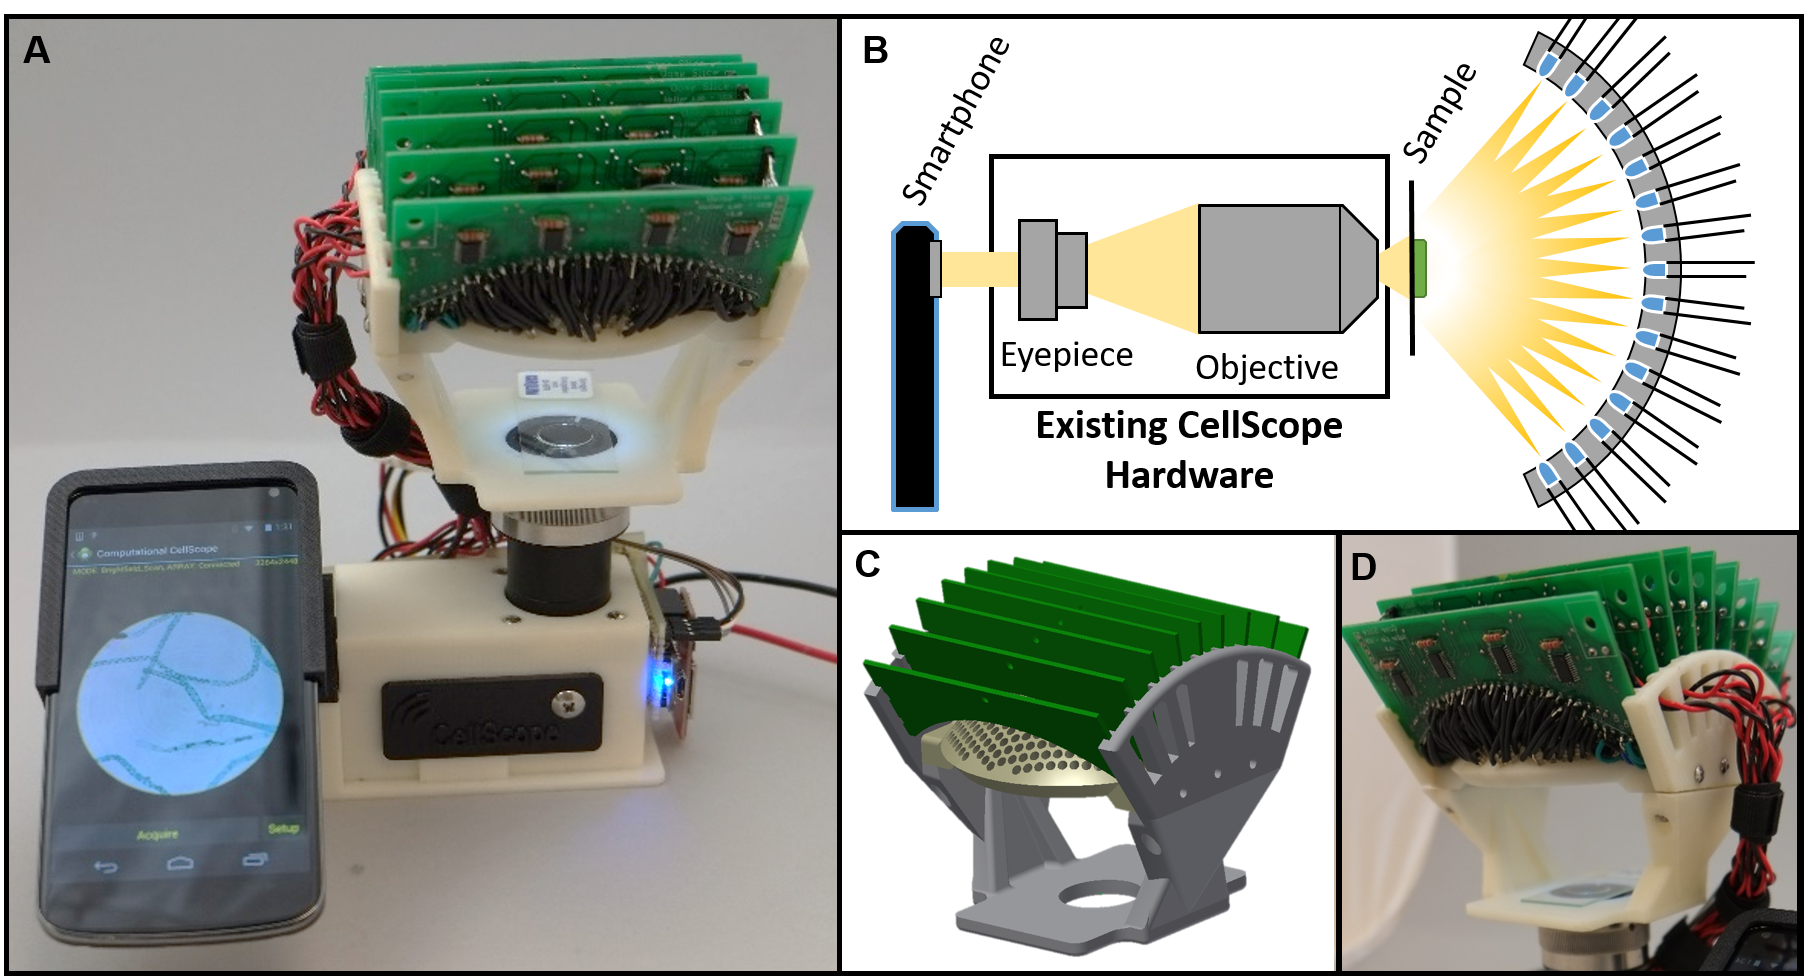
\includegraphics[width=\textwidth]{figures/fig_ccs_system.png}
\end{center}
\caption {{Computational CellScope.} {a).} Device observing a sample using a Nexus 4 smartphone. {b).} Optical schematic of the CellScope device with our custom-made domed LED illuminator. {c).} CAD assembly of the dome. {d).} Assembled dome and control circuitry.}
\label{fig:device}
\end{figure}

% Contrast method comparison figure
\begin{figure}
\begin{center}
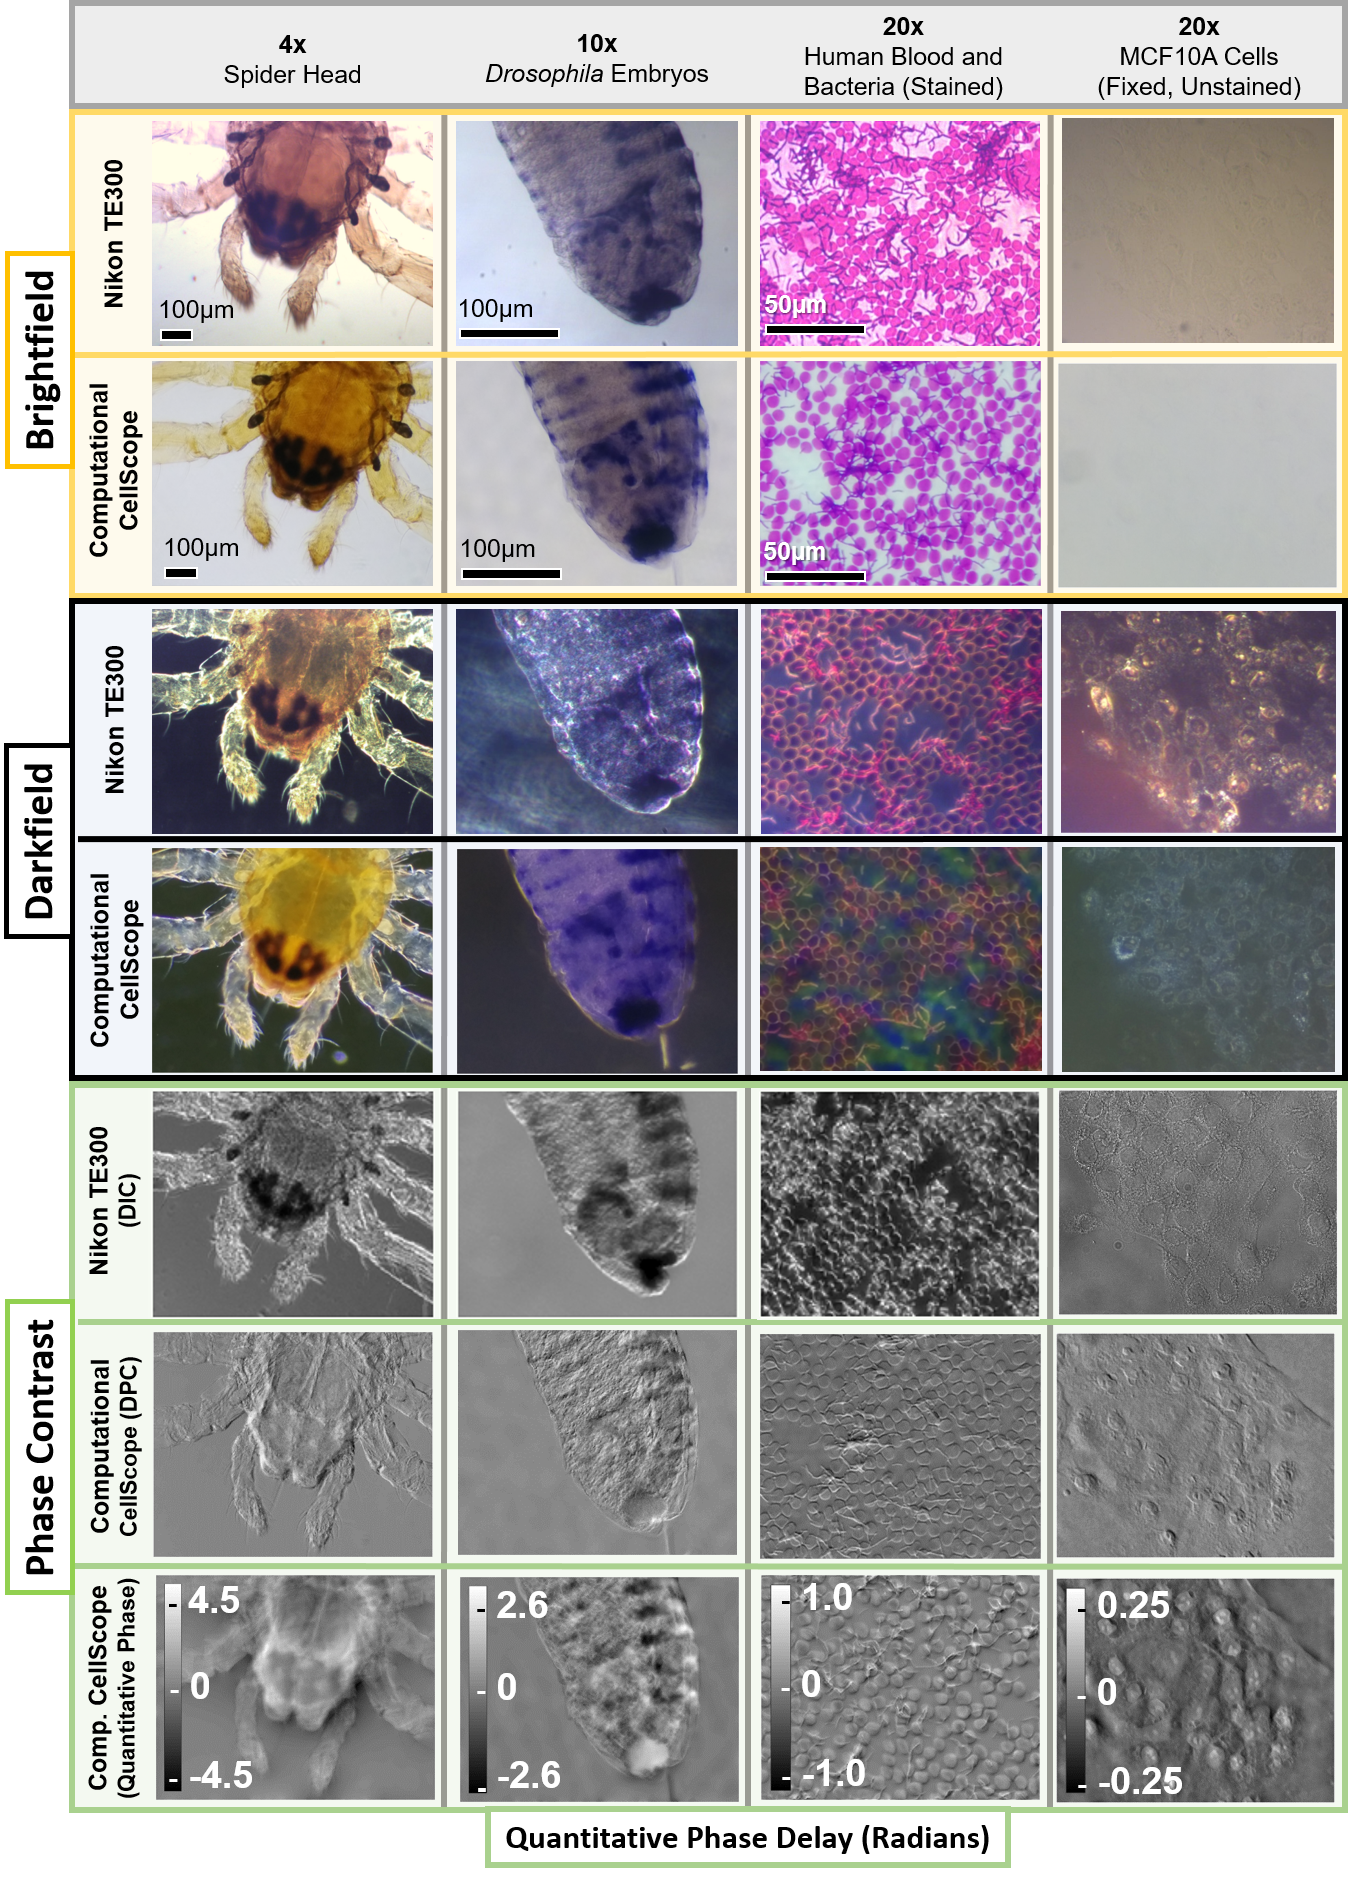
\includegraphics[width=0.67\textwidth]{figures/fig_ccs_mosaic.png}
\end{center}
\caption {{Image Results Compared to a Standard Microscope.} Computational CellScope acquires brightfield and darkfield images of similar quality to a standard upright microscope (Nikon TE300) without the use of hardware inserts. Additionally, it enables phase imaging using Differential Phase Contrast (DPC), which contains similar information to standard phase contrast imaging, and can be inverted to obtain quantitative phase of the sample (bottom row). Differences in color shades are caused by the relative differences in hue of the halogen lamp and the white LEDs. Note the additional dark features in DIC results, as compared to DPC, illustrating mixing of phase and absorption information in DIC. In the rightmost column, we show images for an unstained transparent sample, illustrating the utility of phase imaging methods for label-free imaging.
}
\label{fig:contrastcomparison}
\end{figure}

\subsection{Multi-Contrast Imaging}

To achieve brightfield, darkfield and phase contrast simultaneously, we time-multiplex images taken with different LED patterns and post-process them on the smartphone to synthesize pseudo-real-time multi-contrast imaging, as in~\cite{zijiMulti}. Brightfield images correspond to illumination by LEDs that lie within the cone of angles described by the objective numerical aperture (NA). Darkfield images are obtained by illuminating the sample from angles beyond the angular acceptance of the objective (Fig.~\ref{fig:fabrication_ccs_dome}a)~\cite{Zheng2011}. Since different objectives have different NA, one must specify in the software which objective is being used, with larger NA corresponding to a larger brightfield region of LEDs. Our dome is designed to enable darkfield contrast for any objective of NA$<0.62$, roughly corresponding to a typical 40$\times$ objective.

Phase contrast can be achieved in a single-shot image by any asymmetric illumination pattern~\cite{kachar1985asymmetric,Dodt01101999}. Here, we choose to employ a differential phase contrast (DPC) scheme~\cite{Hamilton1984a,mehta2009quantitative,Tian14,ford2012phase}, which requires two images having complementary illumination patterns, because it gives good phase contrast at all spatial frequencies and can be quantitatively interpreted. The method involves sequentially illuminating the sample with the two opposite halves of the brightfield circle while capturing an intensity image for each. For example, one may first take an image, $I_\mathrm{R}$, with only the right half of the LEDs on and then a second image, $I_\mathrm{L}$, with only the left half of LEDs on (see Fig.~\ref{fig:fabrication_ccs_dome}b). The two images are processed as follows to obtain brightfield and phase contrast:

\begin{equation}
I_{\mathrm{BF}}=I_\mathrm{L}+I_\mathrm{R}, \qquad I_{\mathrm{DPC}}= \frac{I_\mathrm{L}-I_\mathrm{R}}{I_\mathrm{L}+I_\mathrm{R}},
\label{IBF}
\end{equation}

\noindent where $I_{\mathrm{BF}}$ is the brightfield image and $I_{\mathrm{DPC}}$ is the phase contrast image. Since the LEDs are mutually incoherent, adding the two images gives an equivalent brightfield image and subtracting them produces phase contrast, due to asymmetric clipping in Fourier space. The intensity of the DPC image can be shown to be approximately proportional to the first derivative of phase along the direction of illumination asymmetry~\cite{Hamilton1984a}, and different axes of rotation can be programmed by changing the LED array pattern accordingly. Typically, we capture an additional two images in order to compute both the Left-Right and Top-Bottom phase derivative results representing both orthogonal directions. DPC images are qualitatively similar to Differential Interference Contrast (DIC); however, the latter is not a quantitative method. To obtain quantitative phase from DPC images, we solve the inverse problem~\cite{mehta2009quantitative,tian20153d} using a simple deconvolution in Fourier space, as shown in Fig.~\ref{fig:contrastcomparison}.

Thus, by acquiring two (or four) half-brightfield images and a single darkfield image for each time point, we can synthesize brightfield, darkfield, and phase contrast modes in near real-time. Users have the option of saving and post-processing time-multiplexed frames or viewing a live multi-contrast display of the sample, though display speed is significantly faster in the latter case. We developed an application to stream these four contrast modes size-by-side while updating each frame sequentially as the illumination pattern cycles through the different patterns (Fig.~\ref{fig:android}b). The user may touch any of the four images for a live full-screen display of that contrast mode only, and the illumination pattern cycle will update to reflect this.

Some image results for each of the contrast modes are shown in Fig.~\ref{fig:contrastcomparison}, using different objective magnifications and samples. For comparison, we show the same samples imaged in a commercial inverted microscope with traditional hardware. Darkfield was obtained by using a Ph3 condenser aperture in combination with objectives having NA smaller than the sine of the half-angle of the Ph3 annulus inner diameter. Since DPC is not currently commercially available, we instead compare our DPC phase contrast images to (similar-appearing) DIC. Both provide images whose contrast is related to the first derivative of phase along a single direction; however, DIC mixes absorption and birefringence information with phase, so that dark features in the image may result from either absorption of the sample or phase contrast interferences. In the DPC images, on the other hand, the image is related purely to the sample phase distribution (see Fig.~\ref{fig:contrastcomparison}), which can be inverted to reveal quantitative phase, as shown in the bottom row. Provided in a portable package, these multi-contrast video and streaming methods have the potential to allow clinicians to view a sample with three separate contrast methods at once, enhancing the information available for diagnosis and disease discrimination.

\subsection{Digital Refocusing}
For thick samples, our system can capture a different sequence of images in order to recover 3D images and enable digital refocusing. In this case, we sequentially capture images for each of the LEDs in the brightfield region. The resulting dataset is similar to limited angle tomography with many angles, which provides depth sectioning from angular information~\cite{Kak:1988fk}. For simpler processing more amenable to mobile phone programming, we use a lightfield approach here ~\cite{Ng2005,Zheng2011}. This involves a simple shift-and-add algorithm to digitally refocus the image to different axial ($z$) planes. We calculate the digitally refocused intensity image at a distance $\Delta z$ away from the physical focus plane as:
\begin{equation}
I^{\Delta z} = \sum_{\text{all brightfield LEDs}}I_i(x+\Delta z\tan{\theta_x}, y+\Delta z\tan{\theta_y}),
\label{I_refocus}
\end{equation}
where $I_i$ denotes the intensity image for the $i^{\text{th}}$ LED, shifted according to its angle of illumination at the sample $(\theta_x,\theta_y)$ and the desired refocus distance $\Delta z$.

The number of individual LEDs making up the brightfield region roughly determines the number of depth planes that can be accurately reconstructed, and the range of illumination angles determines the axial resolution of the 3D result. Conveniently, the illumination angles may be flexibly sub-sampled in order to trade off acquisition time for quality of result. Since a separate image is taken for each illumination angle, both acquisition and processing time are a function of the numerical aperture of the objective, as illustrated in Fig.~\ref{fig:android}. Acquisition speed was primarily limited by the time required to save an image to the smartphone’s flash memory at full resolution (8 Megapixels on the Nexus 4). This is important because data acquisition remains fast, while processing can occur in the background. Using the same dataset, we can also calculate 3D phase contrast images by digitally refocusing the two halves of the brightfield region separately~\cite{Tian14}. It is expected that this mode of imaging intensity or phase in 3D with no moving parts will give better diagnostic information for thick samples. Alternatively, it could be used for correcting misfocus, obviating the need for automatic axial translation or automated focus adjustment in long time-lapse studies.

% Digital refocus results figure
\begin{figure}
\begin{center}
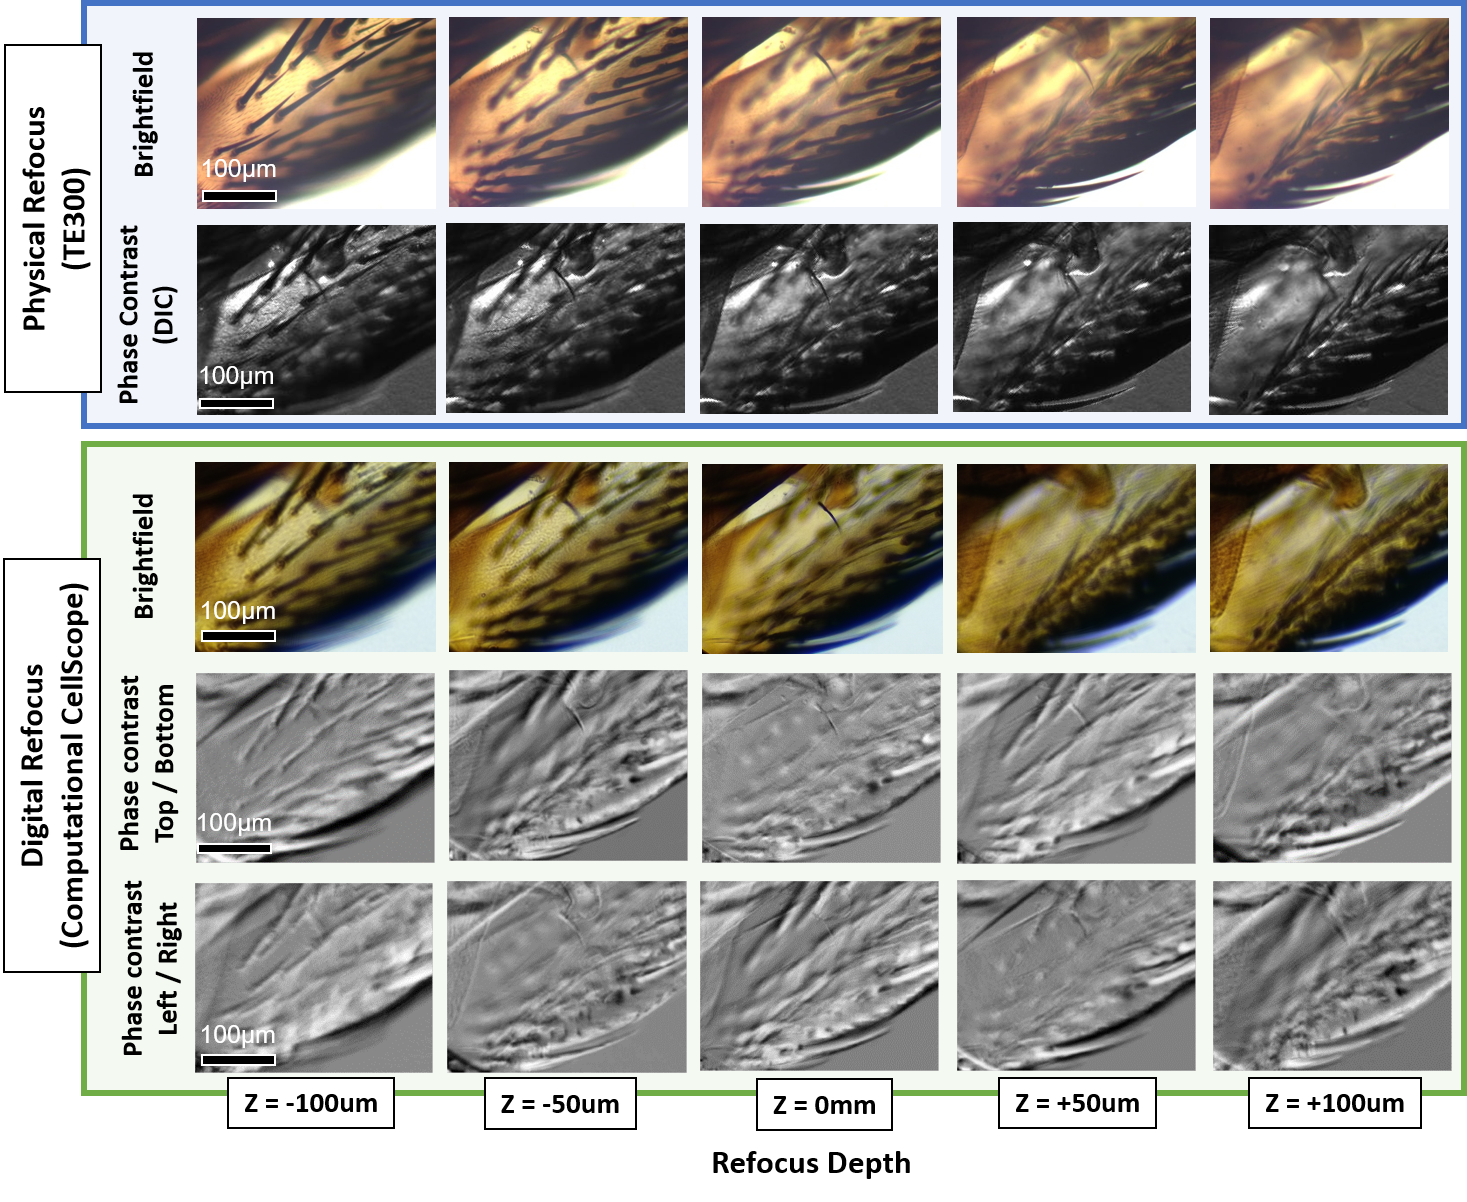
\includegraphics[width=\textwidth]{figures/fig_ccs_refocus.png}
\end{center}

\caption { {Digital refocusing on the Computational CellScope.} Comparison of digital refocusing to physical refocusing on a commercial microscope (Nikon TE300) of a house fly wing sample (AmScope PS200) with a 10$\times$ objective. Digitally refocused phase contrast images are also computed for both vertical and horizontal phase derivatives at different focus depths.}

\label{fig:digrefocus}
\end{figure}

Results are shown in Fig.~\ref{fig:digrefocus} for digitally refocused images as compared to physically refocused images on an inverted microscope (Nikon TE300), both with a 10$\times$ objective (0.25 NA). The phase contrast images show the first derivative of phase along both the vertical and horizontal directions, calculated from the same dataset using only the green color channel. The algorithm successfully refocused features across 400$\mu$m depth of field, limited by object thickness. Our refocusing achieves an axial resolution of approximately 5$\mu$m within $\pm50\mu$m of physical focus position, but degrades approximately linearly with increasing refocus distance~\cite{Tian14}. Processing time is approximately 1.5 minutes per depth slice for a 10$\times$ objective.

\subsection{Hardware Implementation}
The illuminator consists of 4 major components: a hemispherical dome frame for mounting the LEDs, the LEDs themselves, controller circuit boards and the sample stage. The dome mounting structure is a rigid hemisphere designed to constrain the individual LEDs within an array of computationally positioned bores, aligning the LED with the radius vector to the sample center.  This hemisphere was designed with a $60\textrm{mm}$ radius in order to provide maximum intensity at the sample, given our desired number of LEDs and a minimum distance between neighboring LEDs. The part was 3D printed using a SLA printer (InterPro Models) to achieve the necessary 100$\mu$m printing resolution for accurate LED positioning. The LED angular positions were computed algorithmically to ensure uniform spacing across the dome, constrained by a minimum 150$\mu$m distance between bores for mechanical rigidity and a maximum angular separation of 3.85 degrees allowing for sufficient coherence area at the sample. This angular spacing means that 38 LEDs make up the brightfield region for our smallest NA objective (4$\times$), with even more for larger NA objectives, ensuring high quality digital refocusing results across a large range of depth slices for all objectives. The $3\textrm{mm}$ through-hole, white LEDs (Mouser 593-VAOL-3LWY4) were press fit into the dome and a rigid lateral constraint was provided by acrylic retaining inserts behind each individual LED. 508 of these LEDs were soldered directly to controller boards arranged above the array, with insulated leads to prevent electrical shorting.

Accounting for mechanical tolerances of the 3D printed dome and the LED epoxy lenses, manufacturing tolerances suggest that the maximum angular pointing error will be no greater than ±4.8 degrees. This corresponds to a maximum intensity attenuation of only 1.2\% due to assembly variation and tolerances across all illumination angles. Our illumination is also quite uniform across the field of view. The maximum field of view of our optical system has a radius of $1.25\textrm{mm}$, set by the eyepiece field-stop diameter of $10\textrm{mm}$ and assuming a 4$\times$ objective. Given the $60\textrm{mm}$ radius of curvature of our dome, this corresponds to illumination variation due to mechanical tolerances being less than 1\% across the field of view for each single LED illumination.  While this result is quite good, the spread of intensities between different LEDs is significantly larger (see Fig.~\ref{fig:fabrication_ccs_dome}g), as a result of combined mechanical, electrical, and parts tolerances. Conveniently, a one-time calibration sweep of illumination angles, taken with no sample present, is sufficient to allow computational removal of this variation for all practical purposes.

The device used nine identical printed circuit boards placed in a fanned arrangement above the dome, each containing four LED controller chips (Texas Instruments TLC5926) serving up to 64 LEDs. These were controlled by a single Arduino Micro micro-controller, which calculates the appropriate bit pattern based on serial commands from an included Bluetooth transceiver. The array is fully addressable through a standard Bluetooth serial link; no wired connection to the phone is needed, although a powered USB connection is provided to charge the phone’s battery as well, for convenience. We operate the serial output at 115K baud and note that we can update the entire pattern with approximately 100ms latency, although we predefine some of the more complex LED illumination patterns and store them in the Arduino flash memory to further improve acquisition time. Thus our final acquisition time is primarily limited by the smartphone camera rather than the LED array control, so could be improved significantly with future smartphone releases.

The dome's power control board is tolerant of voltages between 7 and 20 VDC to allow compatibility with a large range of power sources, including a standard 12V automotive battery and a 100W wall-plug variable output power supply, as well as many commercially available portable power supplies for consumer electronics. During regular usage, the device requires no more than 2A of current, though it could potentially draw up to 4.8A of current when all LEDs are illuminated. This is not a typical use case, however, since simultaneous illumination inside and outside the objective NA amounts to an undesirable mixing of darkfield and brightfield contrast. Noting that for 4$\times$, 10$\times$, and 20$\times$ objective configurations there are more darkfield than brightfield LEDs, to reduce power consumption we perform darkfield illumination by default using an annulus with a width equivalent to 0.15NA rather than using all of the darkfield LEDs. This moderately reduces the contrast and resolution of darkfield images but significantly reduces power use during the darkfield illumination cycle. We note that the device can operate indefinitely without overheating issues for both multi-contrast and digital refocusing.

% Application Timing and Screenshot figure
\begin{figure}
\begin{center}
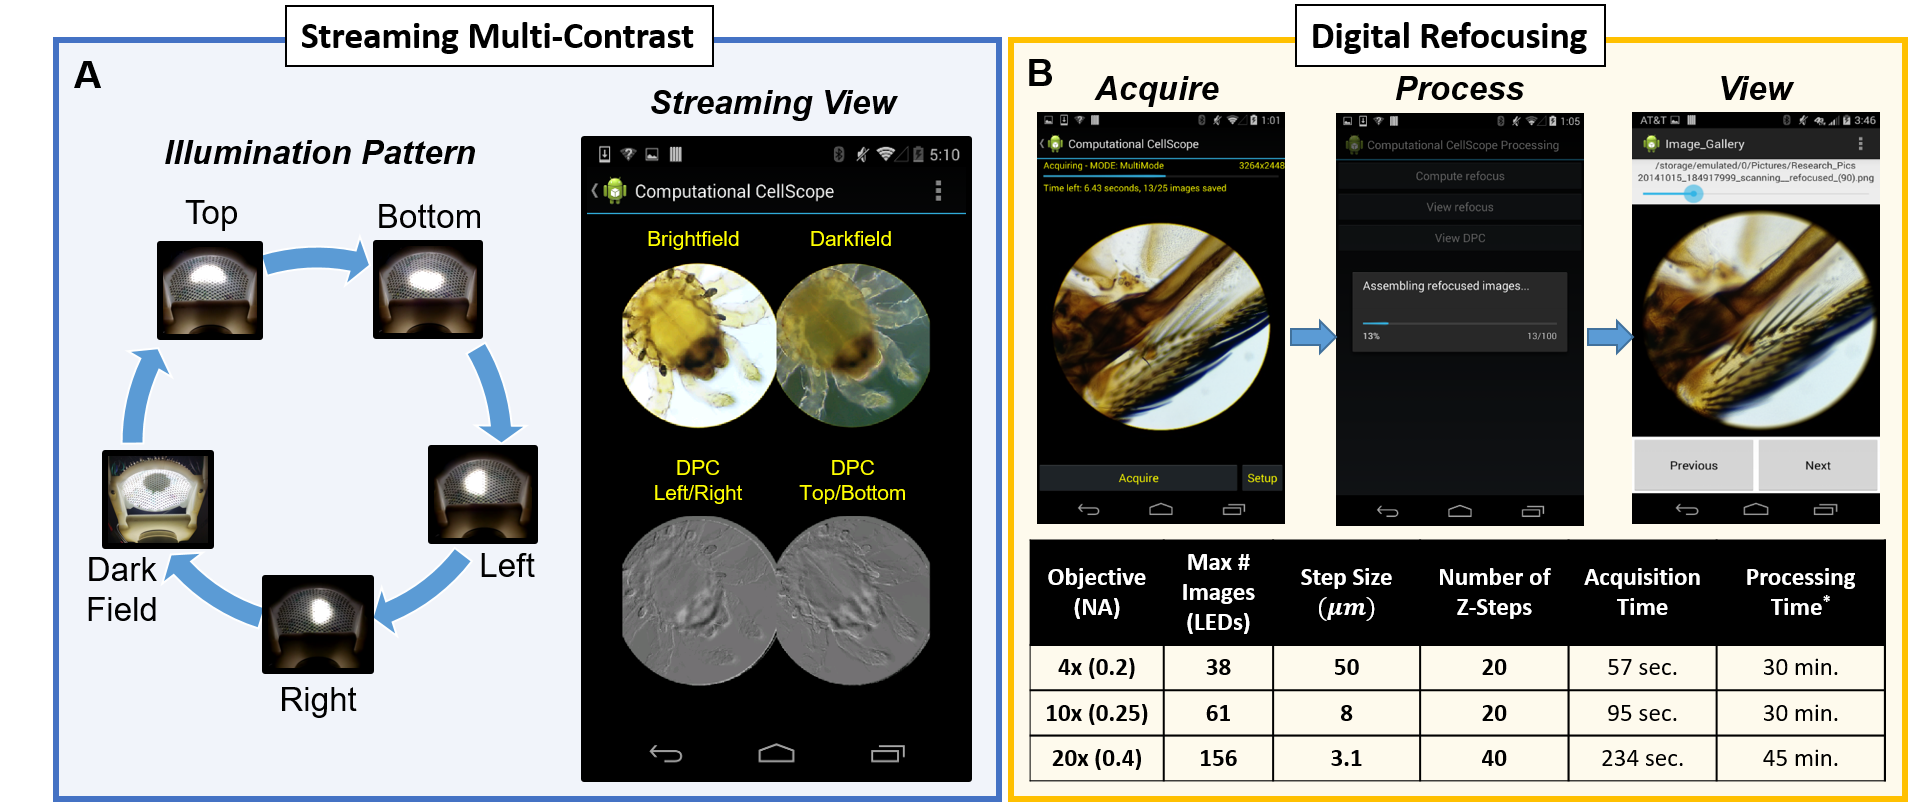
\includegraphics[width=\textwidth]{figures/fig_ccs_app.png}
\end{center}
\caption {{Android Application Workflow.} {a).} Schematic of streaming multi-contrast LED patterns. Here we vary the LED pattern in time and acquire and process images on the smartphone, producing a streaming multi-contrast display of a sample without any further post-processing. The user can touch any image to zoom in and stream an individual image. Total cycle time is 2.3 seconds.
{b).} Overview of workflow for digital refocusing mode. Table shows example processing and acquisition times for a typical dataset reconstruction. Axial Resolution is determined by the range of illumination angles sampled (defined by the objective NA). The number of z-steps were chosen such that refocus blur does not exceed 20 pixels. Processing and acquisition time can be reduced by selecting fewer refocus planes or by sparsely sampling LEDs, trading axial resolution for faster acquisition time.}
%, roughly ¼ the size of a typical 20 $\mu$m cell at 10$\times$

\label{fig:android}
\end{figure}

\subsection{Acquisition Software and Processing}
It has previously been shown that using a smartphone as a microscope poses unique challenges intrinsic to the phone software~\cite{skandarajah2014quantitative}. Smartphone cameras may only allow minimal quantitative control over standard imaging parameters (e.g. focus, exposure, gain), opting for opaque automatic algorithms that simplify the user experience. To circumvent these restrictions, we wrote a custom Android application that attempts to achieve the optimum imaging characteristics with our coded illumination configuration. In addition to a global tap-to-auto-focus capability, specific settings for each acquisition mode are detailed where appropriate in the following discussion. The software application also initiates and handles the Bluetooth connection to the domed array, enabling synchronized acquisition and array control through the standard Android API. Array control is thus transparent to the end-user, requiring them to simply pair the phone with the illuminator and press a connect button to initiate a Bluetooth connection. Our application was developed specifically for the Android platform, and will be compatible with any phone running Android OS version 4.0 or later. However, our algorithms were developed using the OpenCV Library, which is cross-platform for iOS (Apple, Inc.) and other operating systems. Thus most of our application code is portable to other smartphone platforms with moderate development effort. A screenshot of the acquisition and processing are shown in Fig.~\ref{fig:android}. The user may choose to collect and synthesize any or all of darkfield, refocused brightfield and DPC images.

In our application, images were acquired using the standard Android API, which does not provide an interface to set explicit exposure times in lieu of auto-exposure with predefined exposure offset values that are only effective while auto-exposure is active. To circumvent this issue, we included a short pre-illumination sequence before each dataset acquisition to lock exposure at the appropriate value. Additionally, to account for the asymmetric LED packing of our LED array, we choose equal numbers of LEDs for each half-circle used to form DPC images, since DPC requires symmetric and equal illumination. Finally, we incur significant latency between the camera shutter and the availability of the frame to our application within the API, due to post-processing algorithms integral to the phone and performed in the background (e.g. white balance and demosaicing). This severely limits our acquisition speeds, which will likely be improved in newer versions of Android that allow finer camera control through the API. Apple iOS offers a different camera API that may also offer improvements in acquisition speed.

Data post-processing was performed in a standalone Android app, where image stacks were loaded and processed on the phone. We employ a number of functions of the OpenCV Imaging library for Android to perform most of our computation. Individual DPC images are computed in less than a second, as demonstrated in our multi-contrast view mode. Digitally refocusing an image into 21 depth planes (±100 $\mu$m range with 10 $\mu$m sectioning) requires approximately 30 minutes of processing time, but the resulting 3D image stack can be interacted with in real-time; all other computational imaging results are much faster (~ 0.43 frames/sec). The long processing time is attributed to frequent loading and saving to the smartphone’s internal storage. We note that significant improvement in processing speeds for all of our algorithms is possible through implementation using the Android NDK, and is also expected as phone computational power increases with each product generation. These performance metrics were calculated on a Nexus 5 smartphone (LG Electronics) and may vary on other devices.

\section{Summary}
In this chapter, we presented several examples of the fabrication and design process for coded illumination devices. These devices are each the result of many design iterations which incorporate the joint design of hardware and software - a key paradigm of computational imaging. The recent development and commercialization of 3D-printing has enabled rapid prototyping of optical devices, enabling the fabrication and iteration of domed LED illuminators (As show in in Section~\ref{sec:fabrication:ccsdome}). However, due to practical fabrication limitations, we found that reverting to more standardized printed circuit board (PCB) approach (Section~\ref{sec:fabrication:quasidome}) enabled significantly improved manufacturability without significant performance degradation, enabling more rapid dissemination of domed LED illuminators around the world. We also developed coded illumination prototypes with much higher temporal illumination resolution for high-throughput imaging (Section~\ref{sec:fabrication:highthroughput}, which required different design decisions to be made to accommodate rapid temporal coding of LEDs. Finally, in Section~\ref{sec:fabrication:ccs} we described a complete coded illumination solution for portable microscopy using a 3D-printed domed illuminator. This device enabled portable implementations of qualitative microscopy (darkfield and brighfield), quantitative phase imaging using DPC, and 3D digital refocusing of thick samples, all using only the existing smartphone and the addition of our domed illuminator. This device demonstrates how flexible and amenable coded illumination devices can be through example; future work could demonstrate an improved prototype which is fully field-ready in terms of robustness and flexibility, and could enable new applications such as high-throughput imaging and fluorescence imaging.

\chapter{Self-Calibration of Coded Illumination Systems}\label{ch:selfcal}

In Chapter~\ref{ch:introduction}, we described a general computational imaging framework which consisted of both a forward model generation step as well as a computational inversion. In all imaging systems, the forward model is synthesized from the fundamental laws of light propagation (e.g. Maxwell's equations), the optical design of the system, and the accumulated error from optical mis-alignment, dust, manufacturing imperfections, and other sources which can be collectively referred to mis-calibration. While some of these imperfections can be removed using simple processes (such as background subtraction), others, such as system aberrations, are relatively complex, and need to be tolerated or removed using a more sophisticated procedure.

\section{Algorithmic Self-Calibration}
The concept of algorithmic self-calibration (solving jointly for the reconstructed image and the calibration parameters) has proven particularly useful in coherent computational imaging. Examples include probe retrieval in Ptychography~\cite{guizar2008phase, maiden2009improved, tripathi2014ptychographic, Maiden2012}, source recovery for through-focus phase imaging~\cite{jingshan2015partially, zhong2016nonlinear}, pupil and source recovery for Fourier Ptychography Microscopy (FPM)~\cite{Bian:13,Yeh2015,Bian:16}, and calibration-invariant inverse scattering models~\cite{satat2017object}. The standard approach to self-calibration uses alternating projections (AP), which optimizes multiple variables serially, keeping other parameters fixed during each sub-iteration. The non-convexity of AP provides no guarantee of global convergence, but in practice it works with sufficiently diverse data. Self-calibration of aberrations has been demonstrated previously in an LED array microscope for the cases of through-focus phase~\cite{zheng2013characterization} and FPM~\cite{Bian:13,Horstmeyer:14,Ou:14,tian2015computational,Chung:16fluor}, but required a large number of images to be captured. For example, a typical FPM setup~\cite{ou2015high} uses approximately 5$\times$ as many images as our system to achieve the equivalent resolution.

Mathematically, a forward model $\op{A}\{\cdot\}$ can be made a function of any variable, including an arbitrary calibration vector $\vec{c}$, with a simple modification of Eq.~\ref{eq:intro_forward_model}:

\begin{equation}\label{eq:self_calib_forward}
    y = \vec{A}\{\vec{x}; \vec{c}\} + \vec{\eta}
\end{equation}

In the case where $\op{A}$ is differentiable with respect to $\vec{c}$, it becomes possible to recover $\vec{c}$ with knowledge of $\vec{x}$ through direct inversion or gradient methods, though this is only very rarely the case. When $\vec{x}$ is unknown, it becomes necessary to solve for both $\vec{x}$ and $\vec{c}$ using an alternating minimization. When $\vec{c}$ is the point spread function of the system (convolution kernel), this becomes a blind deconvolution problem, which has been extensively studied in both microscopy~\cite{Holmes1992blind, sarder2006deconvolution} and photography~\cite{ayers1988iterative, bell1995information, chan1998total, levin2006blind}. However, $\vec{c}$ can also represent system aberrations~\cite{Ou:14}, illumination parameters such as LED positions~\cite{Yeh2015}, or other parameters.

When $\op{A}$ is differentiable with respect to both $\vec{x}$ (the object) and $\vec{c}$ (the PSF), it can be solved by taking the gradient with respect to $\vec{c}$ and $\vec{x}$ in alternating steps. So long as each gradient step is not too large (or is optimized locally using a line search), this alternating minimization technique will not diverge, and will only improve the initial estimate of $\vec{x}$ and $\vec{c}$ until convergence. However, this alternating approach is non-convex, and therefore is very sensitive to initialization since there are many local minima.

\section{Aberration Self-Calibration using Differential Phase Contrast}\label{sec:selfcal:dpc}

System aberrations are nearly always present in optical systems, and may be field-dependent in some cases (such as low-magnification objectives). When performing DPC, these aberrations can corrupt reconstructions due to model mis-match, especially at high frequencies. It is well-known that aberrations arising from optical mis-alignments can be mostly classified by a small number of Zernicke Polynomials~\cite{ZERNIKE1934689}, which makes these functions particularly well-suited for self-calibration.

In this section, we propose a method of algorithmic self-calibration for Differential Phase Contrast (DPC) microscopy~\cite{kachar1985asymmetric,mehta2009quantitative,tian2015quantitative,Claus2015,chen20163d,PhillipsChen17cDPC}, where we avoid the need for pre-calibration by jointly recovering both the sample's complex-field \textit{and} the spatially-varying aberrations of the system, directly from raw images\footnote{This work was developed in close collaboration with fellow Ph.D. student Michael Chen (Waller Lab, EECS, UC Berkeley).}. The method is an extension of illumination-based DPC microscopy~\cite{mehta2009quantitative,tian2015quantitative}, where images are captured with different source patterns, then a reconstruction algorithm recovers the complex-field. Experiments are implemented in a commercial brightfield microscope with a low-cost programmable LED array light source, such that patterns can be switched quickly with no moving parts~\cite{Zheng2013,Liu2014,tian2015quantitative,tian2015computational}. Among the wide variety of QPI methods, those which use partially coherent illumination, like DPC, are advantageous since they provide 2$\times$ better resolution, more light throughput and reduced speckle~\cite{Wang2011,rodrigo2014rapid,jingshan2015partially,tian2015quantitative}, as compared to coherent methods.


To efficiently recover both the complex field and system aberrations, we employ an AP framework that uses 4 captured images for simultaneous phase retrieval and digital correction of spatially-varying aberrations (Fig.~\ref{fig:self_cal_dpc_joint_estimation}). Three of the measurements are partially-coherent conventional DPC images (with rotated half-circle sources); these provide good phase contrast, but poor aberration contrast. The fourth image uses single-LED (spatially coherent) illumination; this provides aberration contrast, but alone cannot resolve the ambiguity between complex-field and pupil aberration~\cite{lu2016quantitative}. Using both partially-coherent and coherent images together improves sensitivity to aberrations without sacrificing the benefits of partial coherence. We model the aberrations parametrically (with a Zernike basis~\cite{ZERNIKE1934689, zheng2013characterization}) to dramatically reduce the number of unknowns. In addition, by segmenting the field-of-view (FOV), we are able to recover and digitally correct for spatially-varying aberrations across the FOV.

\begin{figure}[ht!]
\centering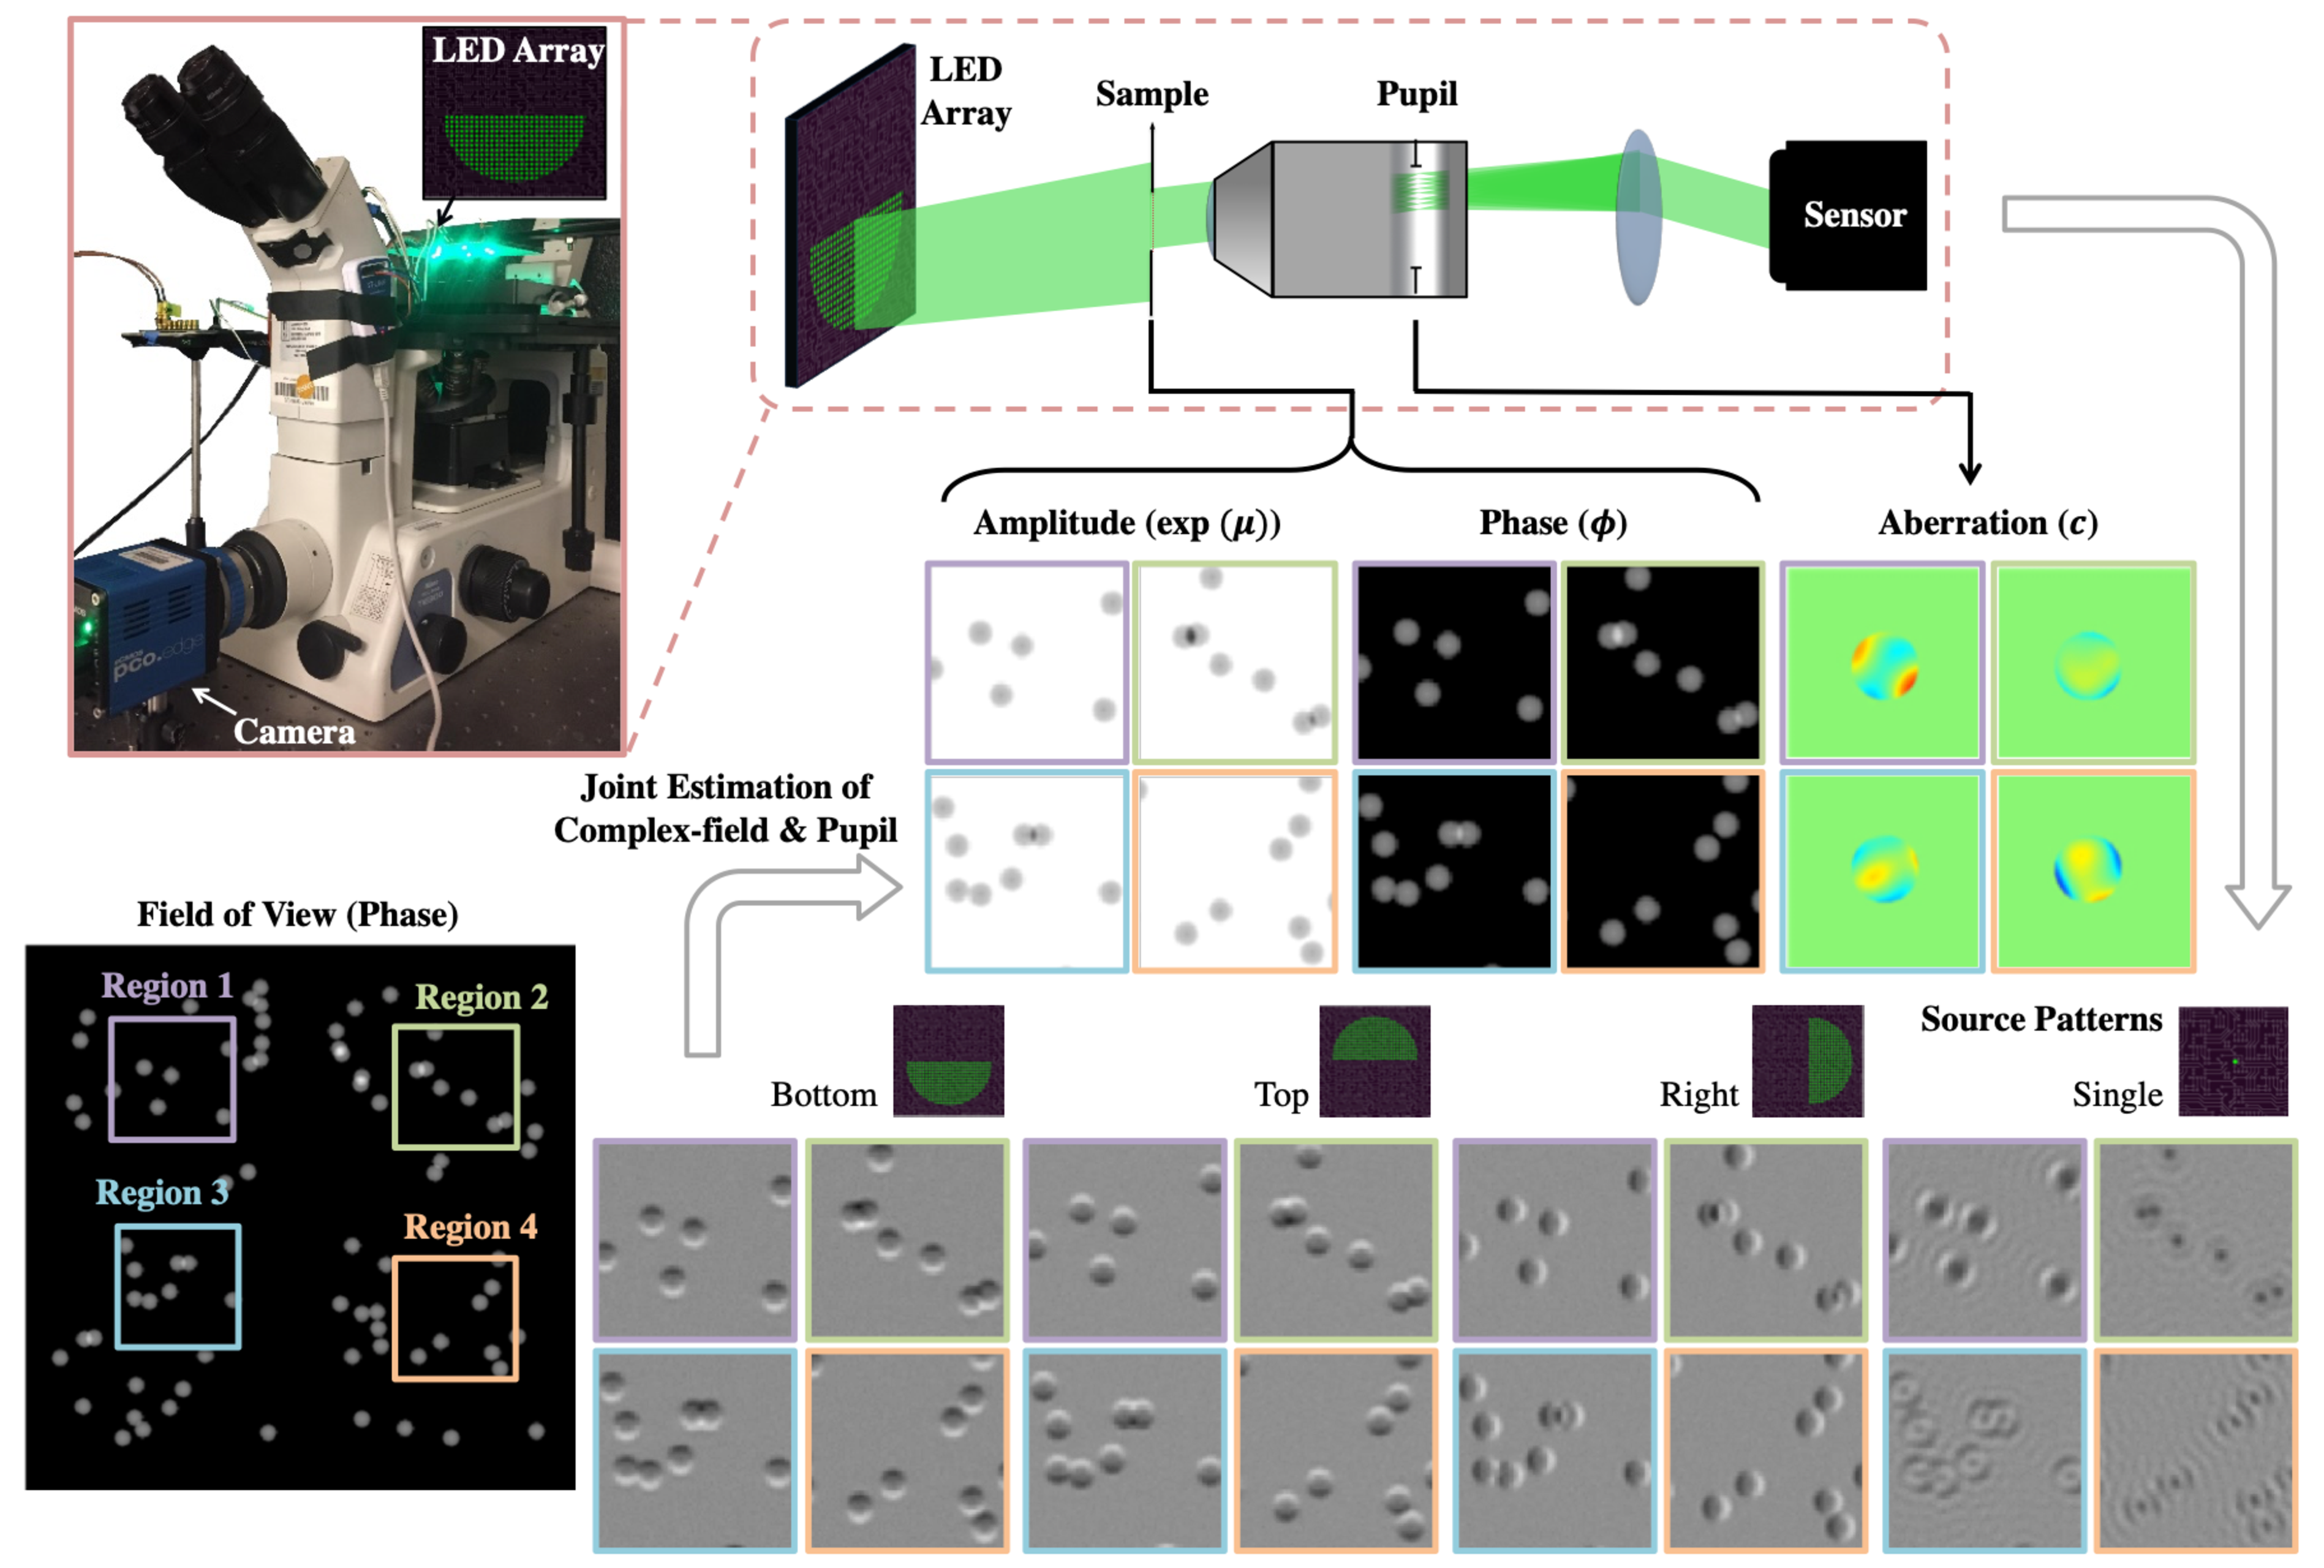
\includegraphics[width=0.9\textwidth]{fig_self_cal_dpc_joint_estimation.pdf}
\caption{\label{fig:self_cal_dpc_joint_estimation} Our LED array microscope captures 4 images with different illumination source patterns (three half-circles and one single LED). The intensity images are used to simultaneously reconstruct both amplitude and phase of the sample, and to estimate the pupil aberrations at each spatial location, which are then digitally corrected for. We show reconstructions for 4 regions with different spatially-varying aberrations.}
\end{figure}

\subsection{Joint Estimation of Complex-Field and Aberrations}

Our LED array microscope and data capture scheme is shown in Fig.~\ref{fig:self_cal_dpc_joint_estimation}. Quantitative DPC (without aberration correction) requires a minimum of 3 intensity measurements to reconstruct phase~\cite{PhillipsChen17cDPC}, though only two quantities (amplitude and phase) are reconstructed at each pixel. Hence, there is significant redundancy in the data which may, in principle, be used to solve for aberrations. Unfortunately, intensity images formed by partially-coherent illumination do not exhibit significant aberration contrast. Hence, we modify the capture scheme to add one additional measurement with spatially-coherent illumination (a single on-axis LED). The example in Fig.~\ref{fig:self_cal_dpc_joint_estimation} has a different aberration in each quadrant of the FOV, and only the single-LED image displays visible differences in contrast for each region. An off-axis LED would also provide the necessary coherent contrast, but the on-axis LED provides higher intensity and better signal-to-noise ratio (SNR). Having achieved both phase and aberration contrast with 1 on-axis and 3 half-circle sources, we use this dataset to jointly recover both spatially-varying aberrations and the complex-field of the sample (with resolution set by the incoherent diffraction limit).

The process of estimating the sample's complex-field and the system's aberrations simultaneously is a joint estimation large-scale nonlinear non-convex problem. To simplify, DPC typically makes a weak scattering approximation which linearizes the forward model. This approximation is generally valid for optically thin or index-matched samples, like biological cells. Intensity measurements can then be related to absorption ($\vec{\mu}$) and phase ($\vec{\phi}$) of the sample~\cite{tian2015quantitative,PhillipsChen17cDPC} by simple convolutions. As derived in Appendix A, the DPC forward model in matrix form is:
\begin{equation}
\label{eq:forwardmodel}
\vec{I}_{\mathrm{n}} = \boldsymbol{\mat{F}}^{-1}\left(\mathrm{diag}(\vec{H}_{\mu})\boldsymbol{\mat{F}}\vec{\mu} + \mathrm{i}\cdot\mathrm{diag}(\vec{H}_{\phi})\boldsymbol{\mat{F}}\vec{\phi}\right)\;.
\end{equation}

\noindent Here, $\mathrm{diag}(\vec{x})$ denotes a diagonal matrix with diagonal values $\vec{x}$, $\boldsymbol{\mat{F}}$ and $\boldsymbol{\mat{F}}^{-1}$ represent the DFT and inverse DFT matrices, $\vec{I}_{\mathrm{n}}$ is the vectorized normalized measured intensity (with the DC term subtracted), and $\vec{H}_{\mu}$ and $\vec{H}_{\phi}$ are vectorized transfer functions for absorption and phase. If the source satisfies the K\"{o}hler illumination configuration, the transfer functions can be numerically evaluated based on the cross-correlation property of Fourier transforms:

\begin{equation}
\label{eq:Hu_matrix}
\vec{H}_{\mu} = \frac{1}{\vec{I}_{\mathrm{o}}}\left[\boldsymbol{\mat{F}}^{-1}\mathrm{diag} (\vec{O}^{*}) \boldsymbol{\mat{F}} + \boldsymbol{\mat{F}}^{-1}\mathrm{diag} (\boldsymbol{\mat{F}}^{*}{\vec{P}}^{*})\boldsymbol{\mat{F}}\mathrm{diag}(\vec{S})\right]\vec{P}\;
\end{equation}

\begin{equation}
\label{eq:Hp_matrix}
\vec{H}_{\phi} = \frac{1}{\vec{I}_{\mathrm{o}}}\left[\boldsymbol{\mat{F}}^{-1}\mathrm{diag} (\vec{O}^{*}) \boldsymbol{\mat{F}} - \boldsymbol{\mat{F}}^{-1}\mathrm{diag} (\boldsymbol{\mat{F}}^{*}{\vec{P}}^{*})\boldsymbol{\mat{F}}\mathrm{diag}(\vec{S})\right]\vec{P}\;,
\end{equation}

\noindent where $*$ is the complex conjugate operation, $\vec{I}_{\mathrm{o}}$ is the total intensity of the source passing through the system, $\vec{S}$ and $\vec{P}$ are the vectorized source and pupil, and $\vec{O} = \boldsymbol{\mat{F}}\mathrm{diag}(\vec{S})\vec{P}$. Typically, the space-invariant exit pupil $\vec{P}$ is a circular function with its radius determined by numerical aperture ($\mathrm{NA}$), and wavelength, $\lambda$. The phase of $\vec{P}$ is the pupil aberration we wish to recover, modeled as a weighted sum of Zernike modes on spatial frequency coordinate ($\vec{u}$)~\cite{ZERNIKE1934689}:

\begin{equation}
\label{eq:Zernike}
\vec{P}(\vec{c}) = \mathrm{Circ}\Big(\frac{\lambda\vec{u}}{NA}\Big)\prod_{m=0}^{M} e^{\mathrm{i}c_{m}\vec{Z}_{m}}\; ,
\end{equation}

\noindent where $M$ is the total number of Zernike modes and $\vec{c}$ contains the coefficients, $c_{m}$, of each orthogonal mode $\vec{Z}_{m}$. To recover spatially-varying aberrations, we solve for individual pupil aberrations at different spatial regions across the FOV and assume the aberrations are locally space-invariant within each region. Given Eqs.~(\ref{eq:forwardmodel})-(\ref{eq:Zernike}), an objective function for the joint optimization of absorption, phase and pupil aberrations can be formulated as:

\begin{equation}
\label{eq:joint_optimization}
\underset{\vec{\mu},\vec{\phi},\vec{c}}{\mathrm{min}} \sum_{s = 1}^{N_{s}} \Big\|\boldsymbol{\mat{F}}\vec{I}_{\mathrm{n},s} - \mathrm{diag}\left(\vec{H}_{\mu,s}(\vec{c})\right)\boldsymbol{\mat{F}}\vec{\mu} -\mathrm{i}\cdot\mathrm{diag}\left(\vec{H}_{\phi,s}(\vec{c})\right)\boldsymbol{\mat{F}}\vec{\phi}\Big\|_{2}^{2} + \tau \op{R}(\vec{\mu},\vec{\phi})\;,
\end{equation}

\noindent where $s$ is the measurement index of each corresponding source pattern, $N_{s}$ is the total number of measurements, $\|\cdot\|_{2}$ represents an $\ell_{2}$ norm, $\tau$ is a regularization parameter and $R$ is a regularization term that helps mitigate noise artifacts. It is inferred from Eq.~(\ref{eq:joint_optimization}) that the aberration coefficients $\vec{c}$ are coupled with both $\vec{\mu}$ and $\vec{\phi}$, so simultaneously optimizing all variables does not guarantee convergence. An alternating projections update strategy instead provides a non-divergence guarantee, as was previously used for phase-from-focus joint source recovery~\cite{zhong2016nonlinear}. Similarly, we iteratively solve for both the complex object and system aberrations as two sub-problems.

Our alternating projections algorithm initializes $\vec{c}$ with zero. At the start of one iteration, the Zernike coefficients $\vec{c}$ are fixed and a DPC deconvolution sub-procedure (Section~\ref{sec:phase}) is performed in order to update the estimates of amplitude, $\exp(\vec{\mu})$, and phase, $\vec{\phi}$. This new complex-field estimate is then held fixed while an aberration estimation procedure (Section~\ref{sec:abber}) is performed. After updating the aberration estimate based on this procedure, a new iteration begins. Eventually, the objective function converges to a stationary point, giving the final estimates of amplitude, phase, and aberration coefficients. In general, this optimization strategy works as long as there exist enough diversity and redundancy in the measurements.

\subsection{DPC phase retrieval sub-procedure}\label{sec:phase}
The phase retrieval sub-procedure amounts to solving the conventional DPC inverse problem~\cite{tian2015quantitative,PhillipsChen17cDPC}, except that it incorporates the current estimate of the Zernike coefficients $\vec{c}_k$ at iteration $k$:

\begin{equation}
\label{eq:phaseretrieval}
\vec{\mu}_{k+1},\vec{\phi}_{k+1} = \underset{\vec{\mu},\vec{\phi}}{\mathrm{arg\; min}} \sum_{s = 1}^{N_{s}} \Big\|\boldsymbol{\mat{F}}\vec{I}_{\mathrm{n},s} - \mathrm{diag}\left(\vec{H}_{\mu,s}(\vec{c}_{k})\right)\boldsymbol{\mat{F}}\vec{\mu} -\mathrm{i}\cdot\mathrm{diag}\left(\vec{H}_{\phi,s}(\vec{c}_{k})\right)\boldsymbol{\mat{F}}\vec{\phi}\Big\|_{2}^{2} + \tau \op{R}(\vec{\mu},\vec{\phi})\; .
\end{equation}

\noindent The regularization term, $R$, should be chosen based on \textit{a priori} information about the sample. For instance, Tikhonov regularization can mitigate noise, and the solution of Eq.~(\ref{eq:phaseretrieval}) can then be found using a non-iterative deconvolution~\cite{PhillipsChen17cDPC}. If the gradients of the object are relatively sparse, the Total Variation (TV) regularizer can be used to reduce noise without degrading edges. Since the regularization term for TV is not differentiable, iterative algorithms for solving Eq.~(\ref{eq:phaseretrieval}) are needed. In this paper, we use the Alternating Direction Method of Multipliers (ADMM) to implement TV regularization~\cite{boyd2011distributed}, typically requiring about 20 iterations.

\subsection{Aberration recovery sub-procedure}\label{sec:abber}
The aberration recovery sub-procedure uses a nonlinear optimization algorithm to update the aberration estimate based on the newly updated complex-field, which is held fixed. The sub-procedure is initialized with the Zernike coefficients estimate from the previous iteration, $\vec{c}_{k}$. Mathematically, the sub-procedure problem is written as:

\begin{equation}
\label{eq:pupilrecovery}
\vec{c}_{k+1} = \underset{\vec{c}}{\mathrm{arg\; min}} \sum_{s = 1}^{N_{s}} \Big\|\boldsymbol{\mat{F}}\vec{I}_{\mathrm{n},s} - \mathrm{diag}\left(\vec{H}_{\mu,s}(\vec{c})\right)\boldsymbol{\mat{F}}\vec{\mu}_{k+1} -\mathrm{i}\cdot\mathrm{diag}\left(\vec{H}_{\phi,s}(\vec{c})\right)\boldsymbol{\mat{F}}\vec{\phi}_{k+1}\Big\|_{2}^{2}\; .
\end{equation}

\noindent Equation~({\ref{eq:pupilrecovery}}) may be solved by a gradient descent (first-order optimization) approach, or more sophisticated second-order optimization routines (\textit{e.g.} Newton's method~\cite{zhong2016nonlinear}). All of these require computation of the gradient of the objective function with respect to $\vec{c}$. If we define the cost function as $f = \sum_{s=1}^{N_{s}}\|\varepsilon_{s}\|^{2}_{2}$, in which $\varepsilon_{s} = \boldsymbol{\mat{F}}\vec{I}_{\mathrm{n},s}-\mathrm{diag}(\vec{H}_{\mu,s})\boldsymbol{\mat{F}}\vec{\mu}_{k+1}-\mathrm{i}\cdot\mathrm{diag}(\vec{H}_{\phi,s})\boldsymbol{\mat{F}}\vec{\phi}_{k+1}$ is the residual vector, the gradient becomes $\nabla_{\vec{c}} f =  \sum_{s=1}^{N_{s}}\left[\partial\varepsilon_{s}/\partial\vec{c}\right]^{\mathrm{H}}\varepsilon_{s}$, where $\mathrm{H}$ denotes Hermitian transpose. Using Eqs.~(\ref{eq:Hu_matrix})-(\ref{eq:Zernike}), the gradient can be calculated analytically as:

\begin{equation}
\label{eq:gradient}
\begin{split}
\nabla_{\vec{c}} f =  \frac{\mathrm{i}}{\vec{I}_{\mathrm{o}}}\boldsymbol{Z}^{\mathrm{T}}\mathrm{diag}(P^{*})\sum_{s=1}^{N_{s}} \Big[&\boldsymbol{\op{F}^{-1}}\mathrm{diag}(\vec{O}_{s})\boldsymbol{\mat{F}}\left[\mathrm{diag}(\boldsymbol{\mat{F}}^{*}\vec{\mu}^{*}_{k+1})-\mathrm{i}\ \mathrm{diag}(\boldsymbol{\mat{F}}^{*}\vec{\phi}^{*}_{k+1})\right]+\\
&\mathrm{diag}(\vec{S}_{s}) \boldsymbol{\op{F}^{-1}}\mathrm{diag}(\boldsymbol{\mat{F}}\vec{P})\boldsymbol{\mat{F}}\left[\mathrm{diag}(\boldsymbol{\mat{F}}^{*}\vec{\mu}^{*}_{k+1})+\mathrm{i}\ \mathrm{diag}(\boldsymbol{\mat{F}}^{*}\vec{\phi}^{*}_{k+1})\right]\Big]  \varepsilon_{s}\; .
\end{split}
\end{equation}

\noindent In this gradient, $\mathrm{T}$ denotes transpose and the Zernike basis, $\mat{Z}^{\mathrm{T}} = [\vec{Z}_{0},\vec{Z}_{1},\ldots,\vec{Z}_{M}]^{\mathrm{T}}$, contains a finite number of modes where $\vec{Z}_{0} \ldots \vec{Z}_{M}$ are the vectorized Zernike modes. For efficient computation, we adopt the L-BFGS algorithm~\cite{LBFGS} and use the gradient in Eq.~(\ref{eq:gradient}) to solve this nonlinear optimization problem, which generally takes $\sim10$ iterations to converge.

\subsection{Simulation results}
To verify the performance of our joint estimation framework, we show simulation results in Fig.~\ref{fig:self_cal_simulation}. The system parameters were chosen to match our experimental setup ($0.4 \mathrm{NA}$, wavelength $514nm$, 177 source LEDs), with the LED array placed sufficiently far away from the sample such that the illumination from each LED is effectively spatially coherent (plane wave)~\cite{Zheng2013,Ou:14,tian2015computational}.

We compare our results with joint phase and aberration recovery FPM in Fig.~\ref{fig:self_cal_simulation}. FPM captures a separate image for each of the 177 LEDs, whereas DPC requires only 4 images to reconstruct the same quantities. FPM intensity images are simulated by using different tilted plane wave illuminations corresponding to each single LED. All the intensity images contain the same pupil aberration, which is a weighted sum of the first 21 Zernike modes. Our simulated DPC measurements are the sum of the intensity images from half-circle blocks of LEDs on the top, bottom, or right regions of the LED array~\cite{tian2015quantitative}. For all measurements, we added synthesized noise using a Poisson distribution with a mean of $\sim$3000 photons per pixel. Equation~(\ref{eq:joint_optimization}) was then solved with $\ell_{2}$ regularization using the 4 DPC images, while we implemented the same algorithm in~\cite{Tian2014} to recover complex-field and aberrations using FPM with the full 177 image dataset. In this setup, FPM could use as few as 32 images (illuminations from the outer-most annular LEDs only) to achieve the same spatial frequency coverage as our DPC method. Therefore, we also include the results of FPM with 32 measurements for comparison.

\begin{figure}[ht!]
\centering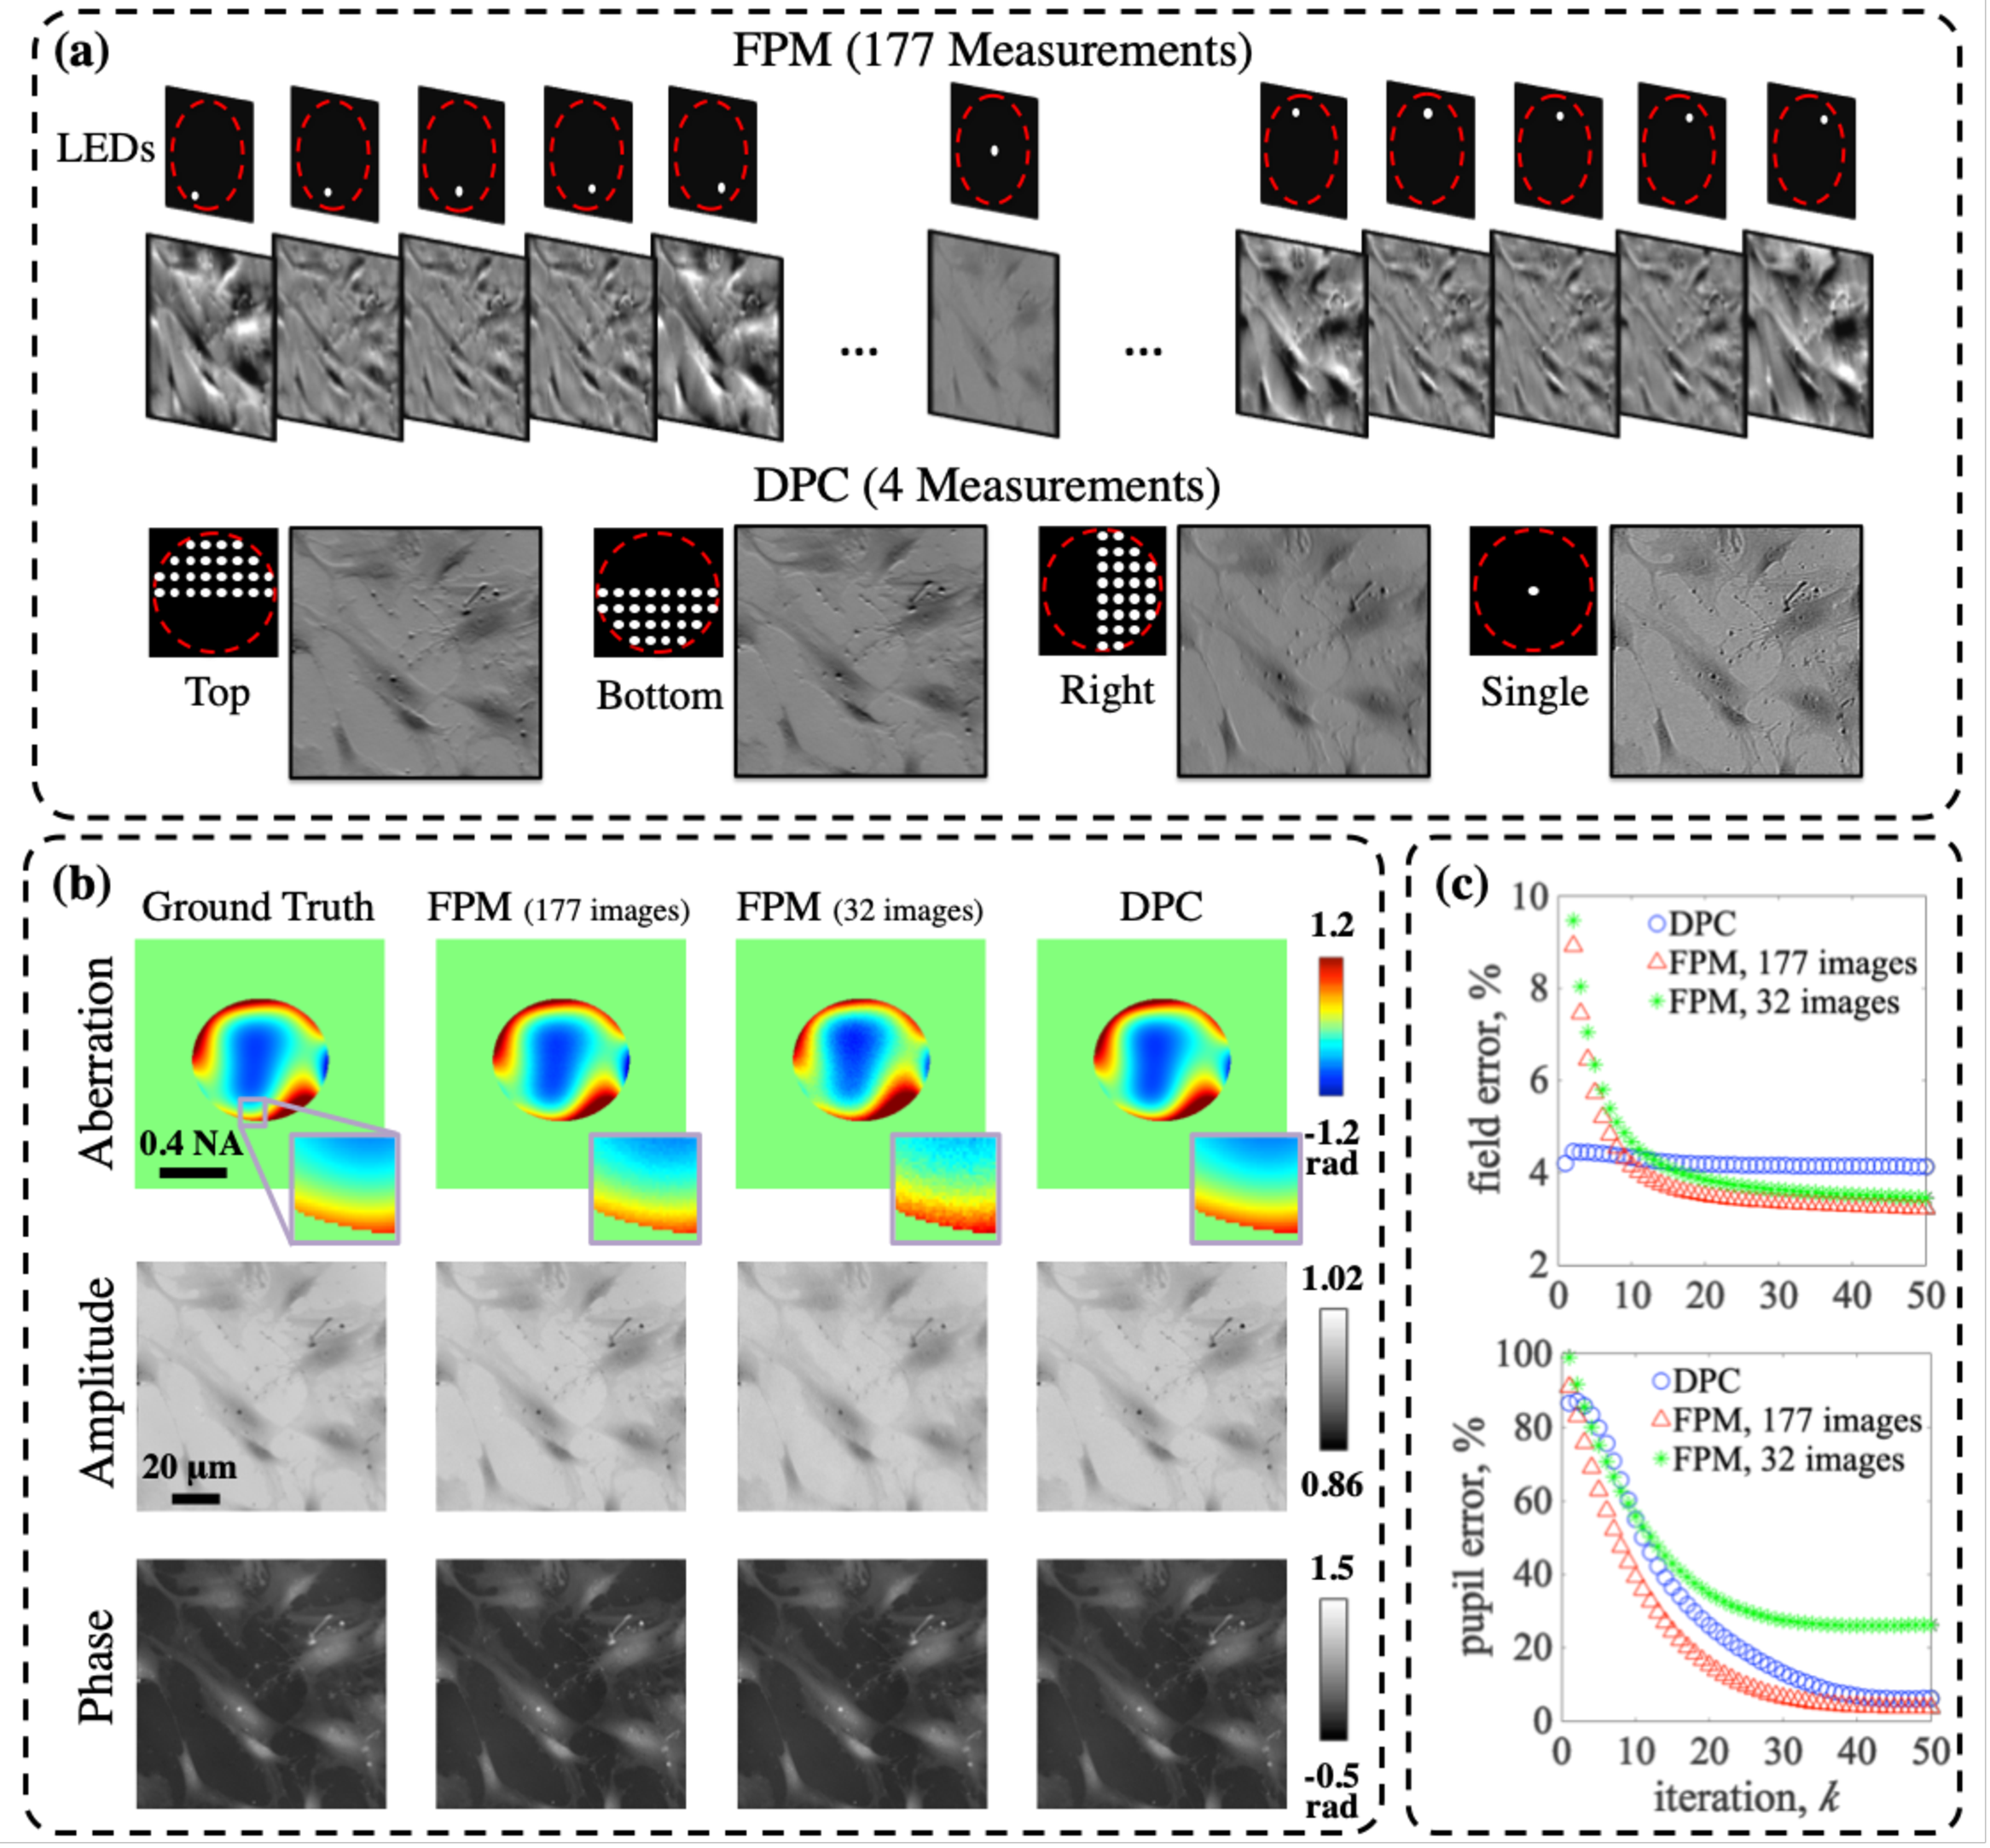
\includegraphics[width=1.0\textwidth]{fig_self_cal_dpc_sim.pdf}
\caption{\label{fig:self_cal_simulation} Performance of joint phase and aberrations estimation on a simulated dataset. (a) Simulated FPM and DPC measurements. Red dashed circles indicate the $\mathrm{NA}$ of the objective lens. (b) Joint estimation of optical field and pupil aberrations, comparing ground truth, FPM and DPC measurements. (c) Errors for complex-field and aberrations at each iteration.}
\end{figure}

Reconstructions from both FPM and our DPC algorithm match the ground truth (See Fig.~\ref{fig:self_cal_simulation}(b)); however, our method only requires 4 measurements, reducing acquisition time and memory requirements. Figure~\ref{fig:self_cal_simulation}(c) plots the normalized root-mean-square error ($\|\vec{x}-\vec{x}_{\mathrm{true}}\|_{2}/\|\vec{x}_{\mathrm{true}}\|_{2}$) at each iteration for both complex-field and pupil aberrations. FPM incurs lower complex-field error than DPC, likely due to both the weak scattering approximation and the larger dataset. As for the pupil aberration error, FPM performance varies significantly with dataset size. While FPM with the full dataset outperforms the proposed DPC framework, our method provides a better result than FPM with 32 images. This is because FPM with fewer measurements has lower effective SNR, adding noise to the recovered pupil aberration (inset of Fig.~\ref{fig:self_cal_simulation}(b)). Our method requires significant computation since it solves two optimization problems at each iteration, but the computation time is comparable to a sequential FPM reconstruction. Both methods were implemented in MATLAB on a desktop computer (Intel Core i7 CPU, Nvidia Tesla C2075 GPU). With a 650$\times$584 pixel object, each iteration took 2.2s for FPM and 2.5s for our DPC algorithm.

\subsection{Experimental results}

Experimentally, we use an LED array microscope with the illumination module replaced with a custom-built LED array ($\lambda = 0.514\mu m$)~\cite{tian2015quantitative, tian2015computational}. A phase target (Benchmark Technologies), which contains periodic patterns of continuous spatial frequencies, is imaged by a $20\times$ $0.4 \mathrm{NA}$ objective lens (Nikon, CFI Plan Achro) in a Nikon TE300 microscope and images are recorded by a PCO.edge 5.5 sCMOS camera on the front port of the microscope (which adds $2\times$ magnification). To test the weak phase gradient assumption, phase images of 6 resolution targets of different heights are recovered using DPC. After validating the reconstructed phase values against theoretical ones, we find that DPC provides accurate results when the phase of the sample is below $0.64$ radians, then underestimates the phase values due to breakdown of the approximation (see Visualization 1). We collect 177 measurements by scanning individual LEDs within a maximum $0.4 \mathrm{NA}$ illumination angle. To provide a fair comparison, we use the same measurements to synthesize the 4 images for our method. As shown in Fig.~\ref{fig:self_cal_dpc_experimentalresults1}(a), DPC measurements with half-circle source patterns have high resolution and qualitatively reveal the phase gradients of the sample, while measurements with single-LED illumination have lower resolution. Two single-LED image zoom-ins that contain the same structure at different orientations are shown in Fig.~\ref{fig:self_cal_dpc_experimentalresults1}(a). One has high contrast, while the other does not, because of directional aberrations. By processing the images using the FPM algorithm and the proposed method with TV regularization, we recover the phase of the sample as shown in Fig.~\ref{fig:self_cal_dpc_experimentalresults1}(b). The FPM and DPC reconstructions are similar, and can resolve features with period as small as $\lambda/\left(2\times NA\right) = 0.643\mu m$. In addition, both results provide reliable quantitative phase of the sample. The refractive index of the binary phase target is 1.52, with height of $100 nm$, resulting in $\sim$0.64 radians peak-to-valley. Looking at the 1D cut-lines (taken along dashed lines) in Fig.~\ref{fig:self_cal_dpc_experimentalresults1}(b), after subtracting the mean of each, the reconstructions show good agreement with the ideal height.

Pupil aberrations recovered by both FPM and DPC algorithms are in Fig.~\ref{fig:self_cal_dpc_experimentalresults1}(c). While we have no ground truth, aberrations estimated from FPM and DPC match well within the $4^{th}$ radial degree of Zernike modes. The dominant aberration in the objective lens is the $8^{th}$ Zernike mode (horizontal coma); this agrees with the evidence of directional aberration mentioned above. One reason causing a difference between the reconstructed pupils is the high-frequency fluctuation shown in the pupil aberration from FPM, which does not exist in the low-order Zernike modes. Although high-order aberrations might be estimated with more measurements to avoid overfitting, it's usually enough to improve image quality by correcting the low-order aberrations.

\begin{figure}[ht!]
\centering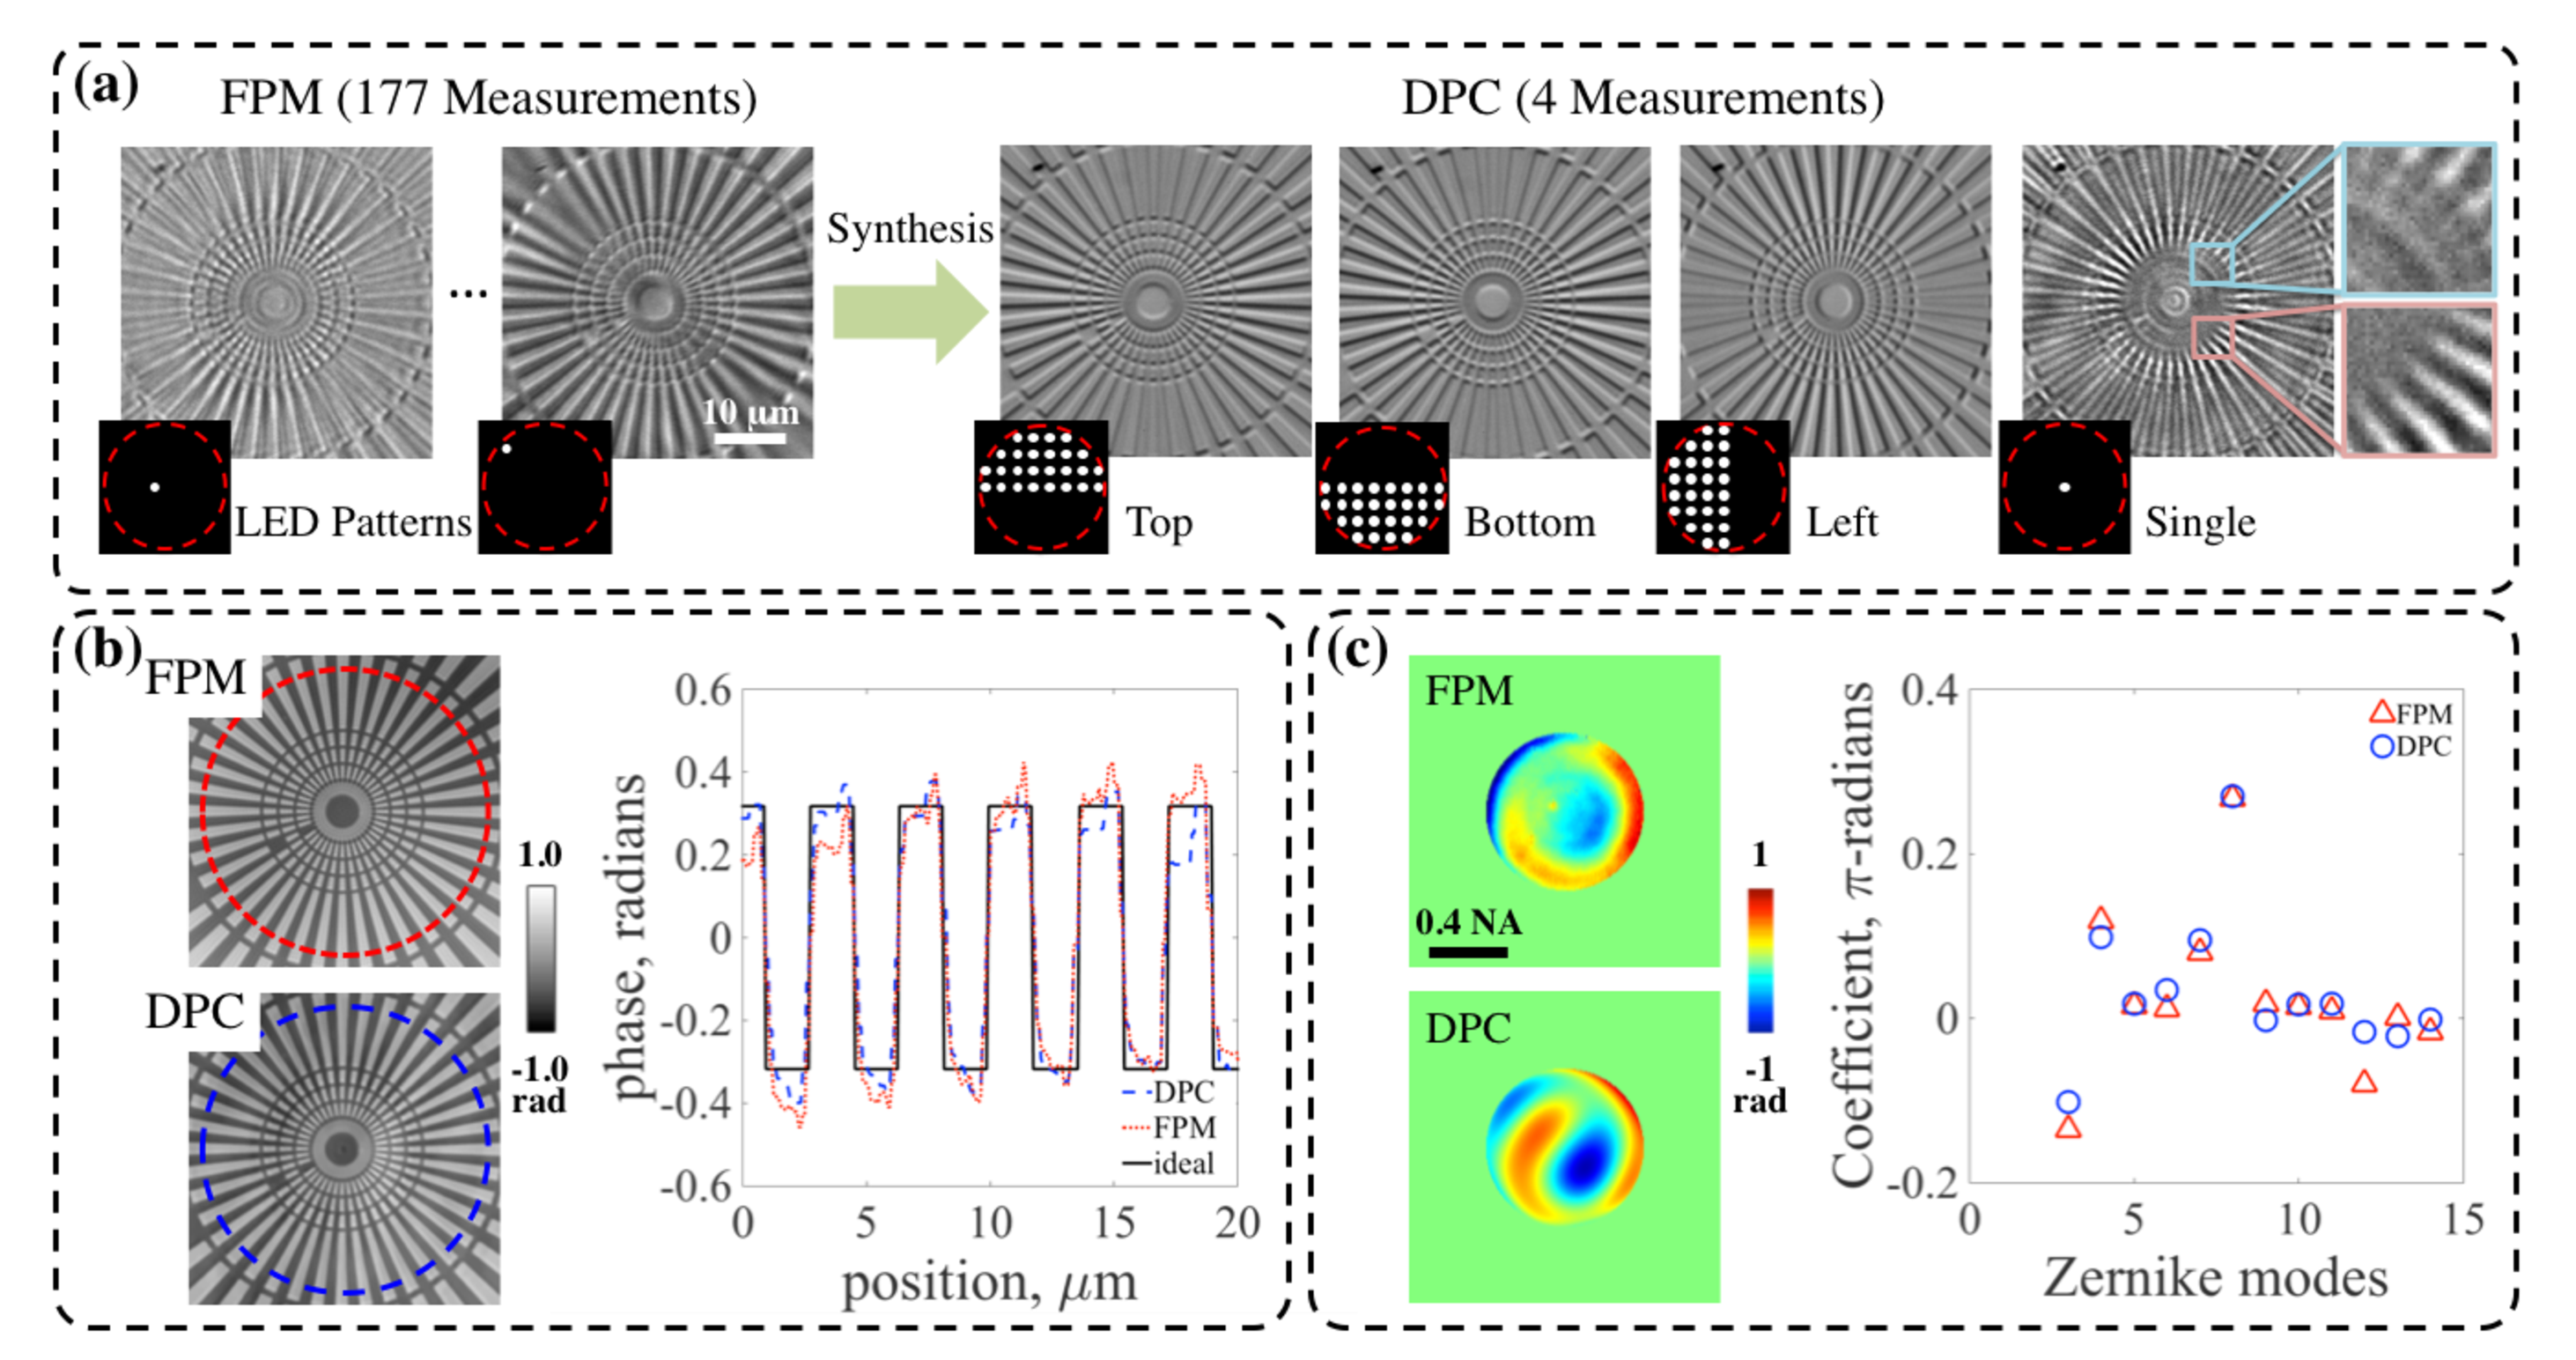
\includegraphics[width=1.0\textwidth]{fig_self_cal_dpc_results1.pdf}
\caption{\label{fig:self_cal_dpc_experimentalresults1} (a) Experimental FPM and DPC measurements for different LED source patterns. Zoomed regions at different orientations for coherent illumination are marked in cyan and pink boxes, respectively. (b) Quantitative phase of a star target using FPM and DPC, along with 1D cutlines for FPM (red) and DPC (blue) along the dashed lines. (c) Reconstructed wavefront error function and the weights of each Zernike mode up to the $4^{th}$ radial degree.}
\end{figure}

To quantify the performance of our method, we introduced known defocus aberrations using an axial motion stage (Thorlabs, MZS500-E). We translated the phase test target across a range of known axial steps over a total range of $40 \mu m$. Each $2 \mu m$ of translation, the 4 images for our method were acquired using a $10\times$ $0.25 \mathrm{NA}$ objective lens (Nikon, CFI Plan Achro) at an acquisition rate of 20Hz. Quantitative phase reconstructions assuming zero aberration, aberration-corrected phase images and the recovered aberrations are shown in Fig.~\ref{fig:self_cal_dpc_experimentalresults2}(a). With increased defocus, the uncorrected phase results degrade. Though our method also suffers from resolution degradation at large defocus distances ($\pm 20\mu m$), it provides better resolution than the uncorrected phase retrieval. For example, in Fig.~\ref{fig:self_cal_dpc_experimentalresults2}(b) the numbers in group 9 are resolved with pupil correction, while they are not readable in the uncorrected result.

We can also recover the focus distances from the defocus term of the Zernike modes and compare the estimated defocus values to known values (Fig.~\ref{fig:self_cal_dpc_experimentalresults2}(c)). Since the Zernike basis is normalized in a range from -1 to 1, the defocus value, $d$, at each time point, $t$, can be evaluated as $d(t) = c_{4}(t)\times\lambda/\pi/(1 - (1 - \mathrm{NA}^{2})^{0.5})$. As expected, the predicted pupil aberrations have quadratic form, which indicates that defocus dominates. Experimentally, our method overestimates defocus values by a factor of 1.16. This discrepancy might originate from mis-calibration of the experiment or parameters used in computation (\textit{e.g.} wavelength, $\mathrm{NA}$ of the objective lens, precision of the motion stage). This linear relationship between the predicted positions and the true focus holds when the magnitude of defocus is less than 16 $\mu m$, $\sim$2$\times$ Depth of Field (DoF). However, the accuracy of aberration correction drops as the defocus value exceeds 2$\times$ DoF, when the maximum phase difference in the pupil becomes larger than 2$\pi$ and the algorithm becomes more likely to converge to a local minimum. From these experiments, we conclude that our method accurately estimates time-varying aberrations within a total range of 4$\times$ DoF.

\begin{figure}[ht!]
\centering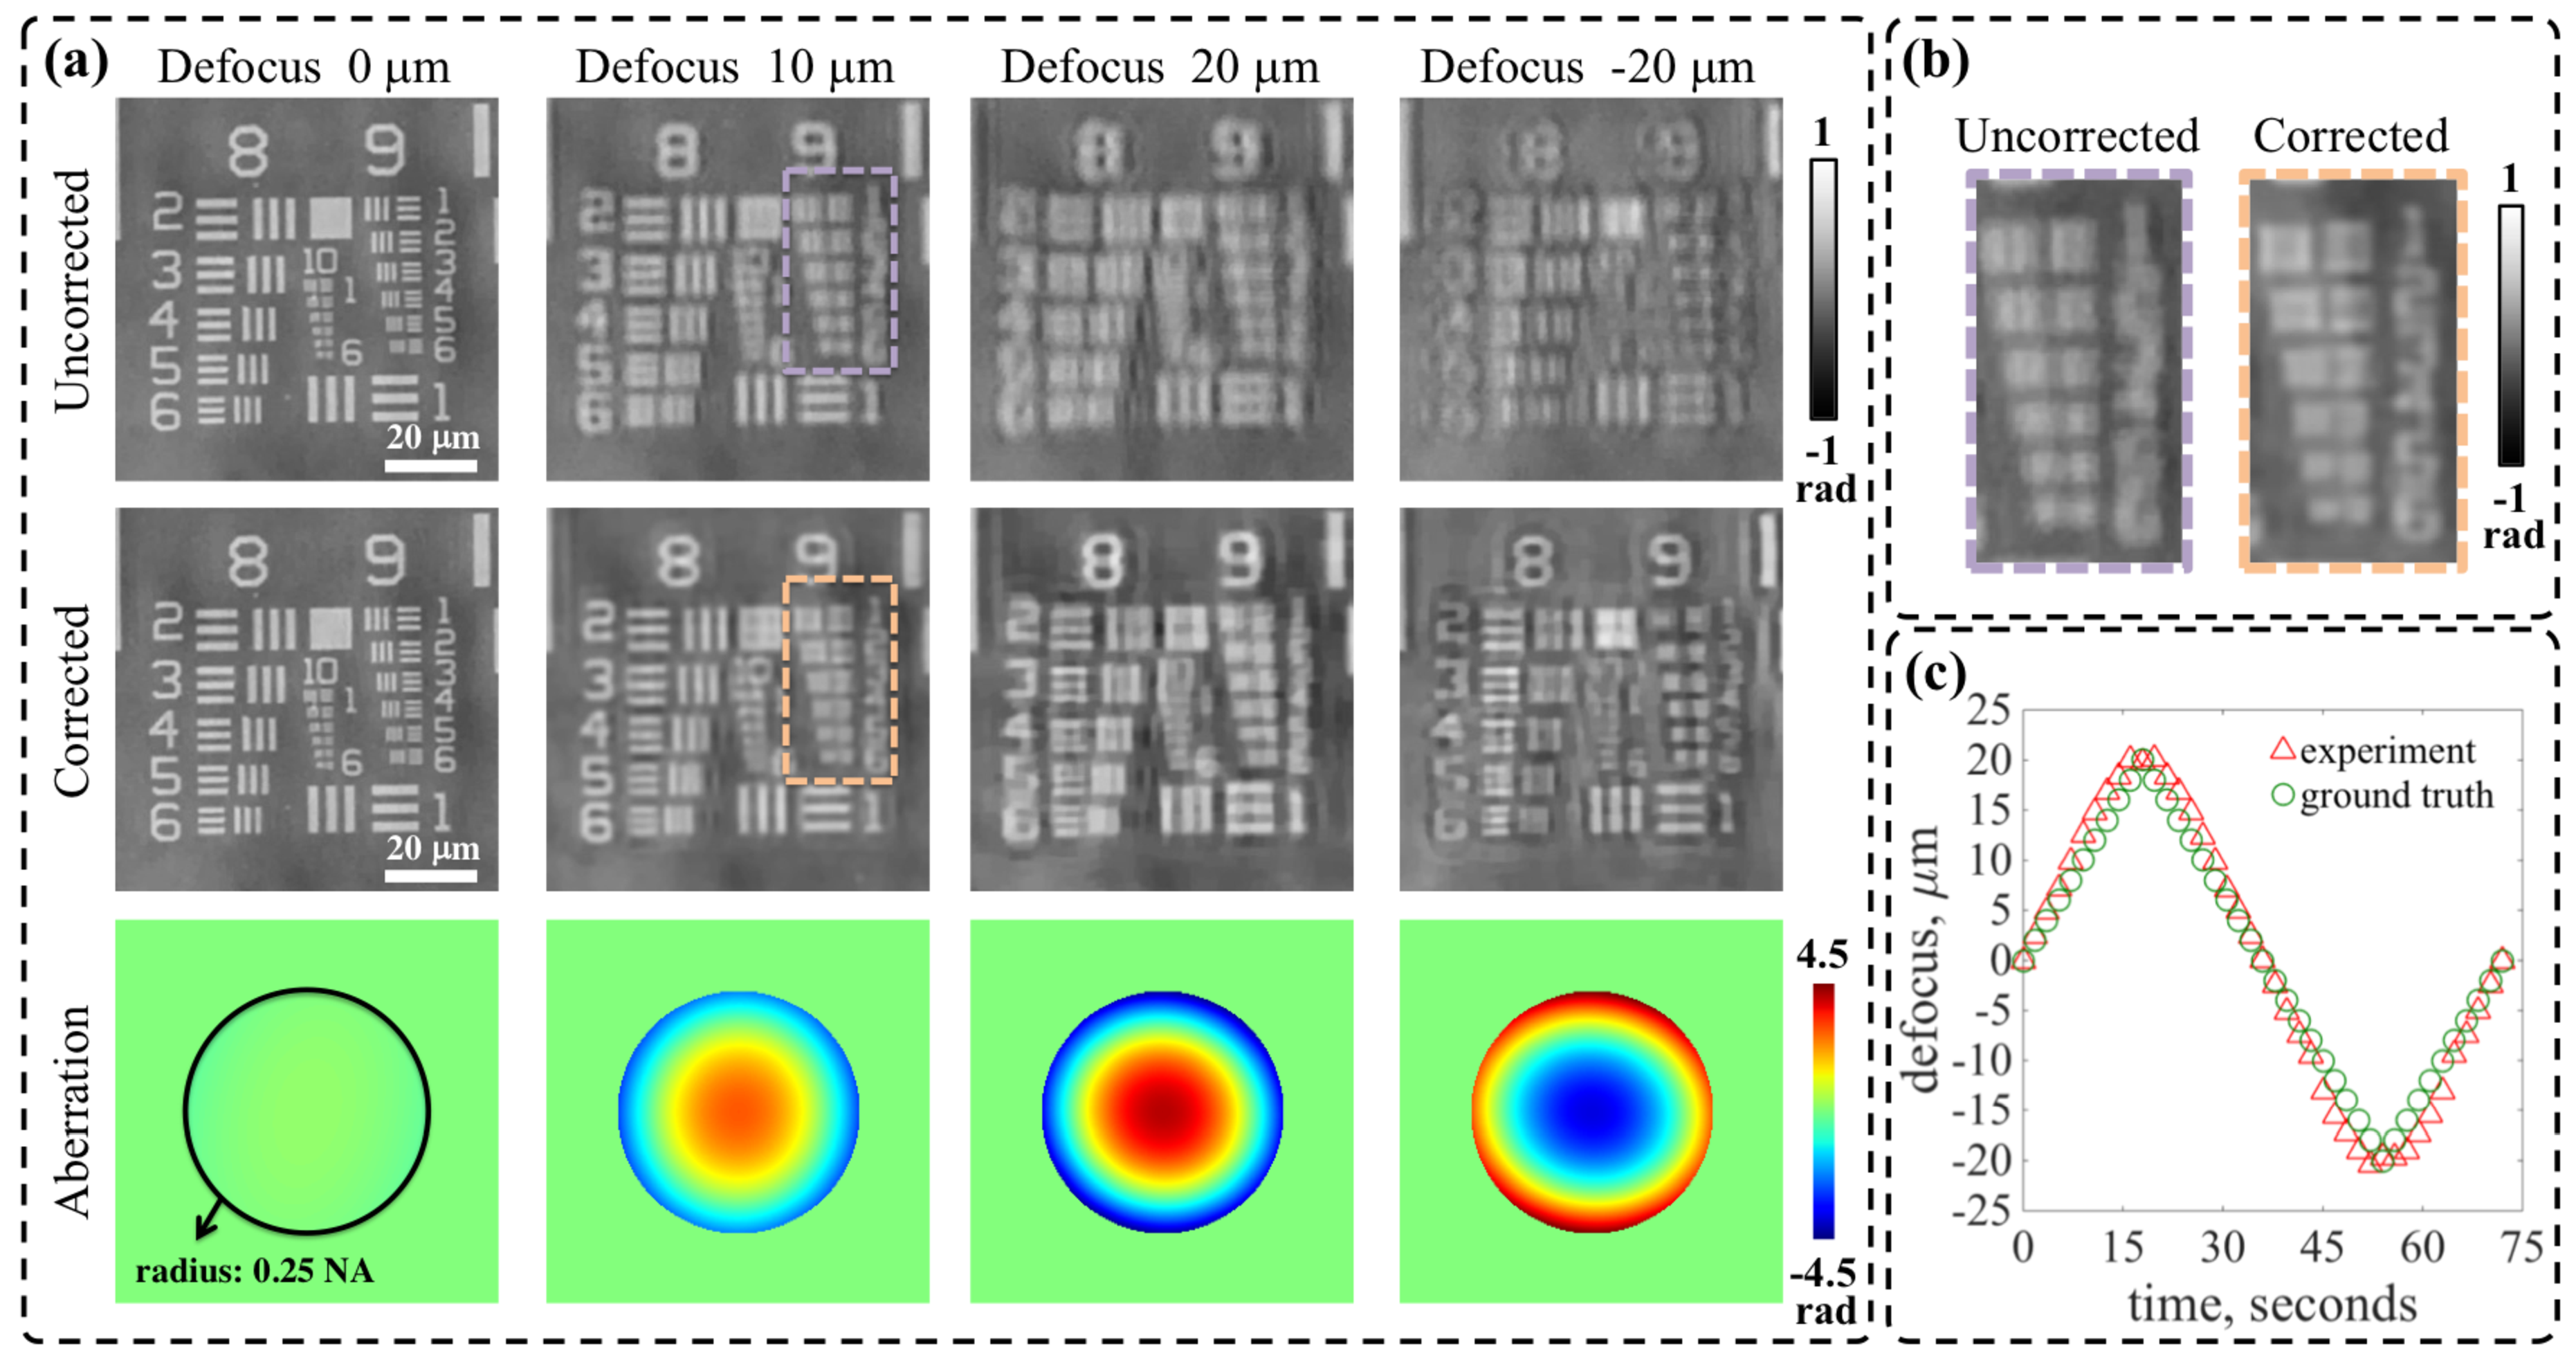
\includegraphics[width=1.0\textwidth]{fig_self_cal_dpc_results2.pdf}
\caption{\label{fig:self_cal_dpc_experimentalresults2} (a) Quantitative phase reconstructions of a USAF 1951 resolution target at various defocus distances with and without aberration correction, and the corresponding recovered aberrations (see Visualization 2). (b) Zoomed-in reconstructions at defocus of $10 \mu m$. (c) Known and experimentally-estimated defocus values from the $4^{th}$ Zernike mode over time.}
\end{figure}

Our method is easily extended to account for spatially-varying aberrations, simply by solving the joint estimation problem separately over different patches of the FOV. In order to visualize spatially-varying aberrations, we prepared oil (Cargille, $\mathrm{n}_{\mathrm{D}}=1.58$) immersed $10\mu m$ polystyrene beads (Sigma-Aldrich) as our sample, which is assumed to be nearly spatially invariant. The sample was imaged by a $4\times$ $0.2 \mathrm{NA}$ objective lens (Nikon, CFI Plan Apo Lambda) that has a FOV of 1.7 $\times$ 2.1mm. Four images were captured at 12.5Hz using the same source patterns as in Fig.~\ref{fig:self_cal_dpc_experimentalresults1}(a). Field-dependent aberrations are primarily caused by two types of system imperfections. First, the incident angle of individual LEDs changes from one FOV to another, since the relative position between the LEDs and the sample at each FOV varies. Second, thecd ..re exist spatially-varying aberrations native to the optical system. To accommodate this spatial variance, we break the full FOV into small patches, and apply the joint estimation algorithm on each patch independently. In this case, the incident angle of individual LEDs and the aberrations are assumed invariant within the patch, which is usually valid when the region is much smaller than the total FOV. In Fig.~\ref{fig:self_cal_dpc_experimentalresults3}(a), the full FOV is divided into 100 patches. Within each patch, the absorption, phase and pupil aberration were recovered independently before being stitched together to form the full FOV images. In practice, optimization for each patch converges in $20-30$ iterations.

Looking at the aberrations recovered, the center of the FOV is essentially aberration-free, which is consistent with the fact that optical systems are usually optimized there. Therefore, the absorption and phase images with pupil recovery are similar to that without aberration correction. Aberrations are much stronger along the edges of the FOV, where the field curvature blurs the image. Consequently, obvious differences occur between the normal DPC and aberration-corrected DPC reconstructions at those patches. The recovered amplitude (absorption) at the bottom right corner is dramatically changed after applying aberration correction. Qualitatively, the uncorrected absorption at the edge of the field appears to contain some phase information, leading to a shadow-like appearance; these artifacts are removed with pupil recovery. In addition, while aberrated phase evaluated with Tikhonov deconvolution suffered from high-frequency noise, phase with pupil correction shows reduced noise due to the use of TV regularization.

\begin{figure}[ht!]
\centering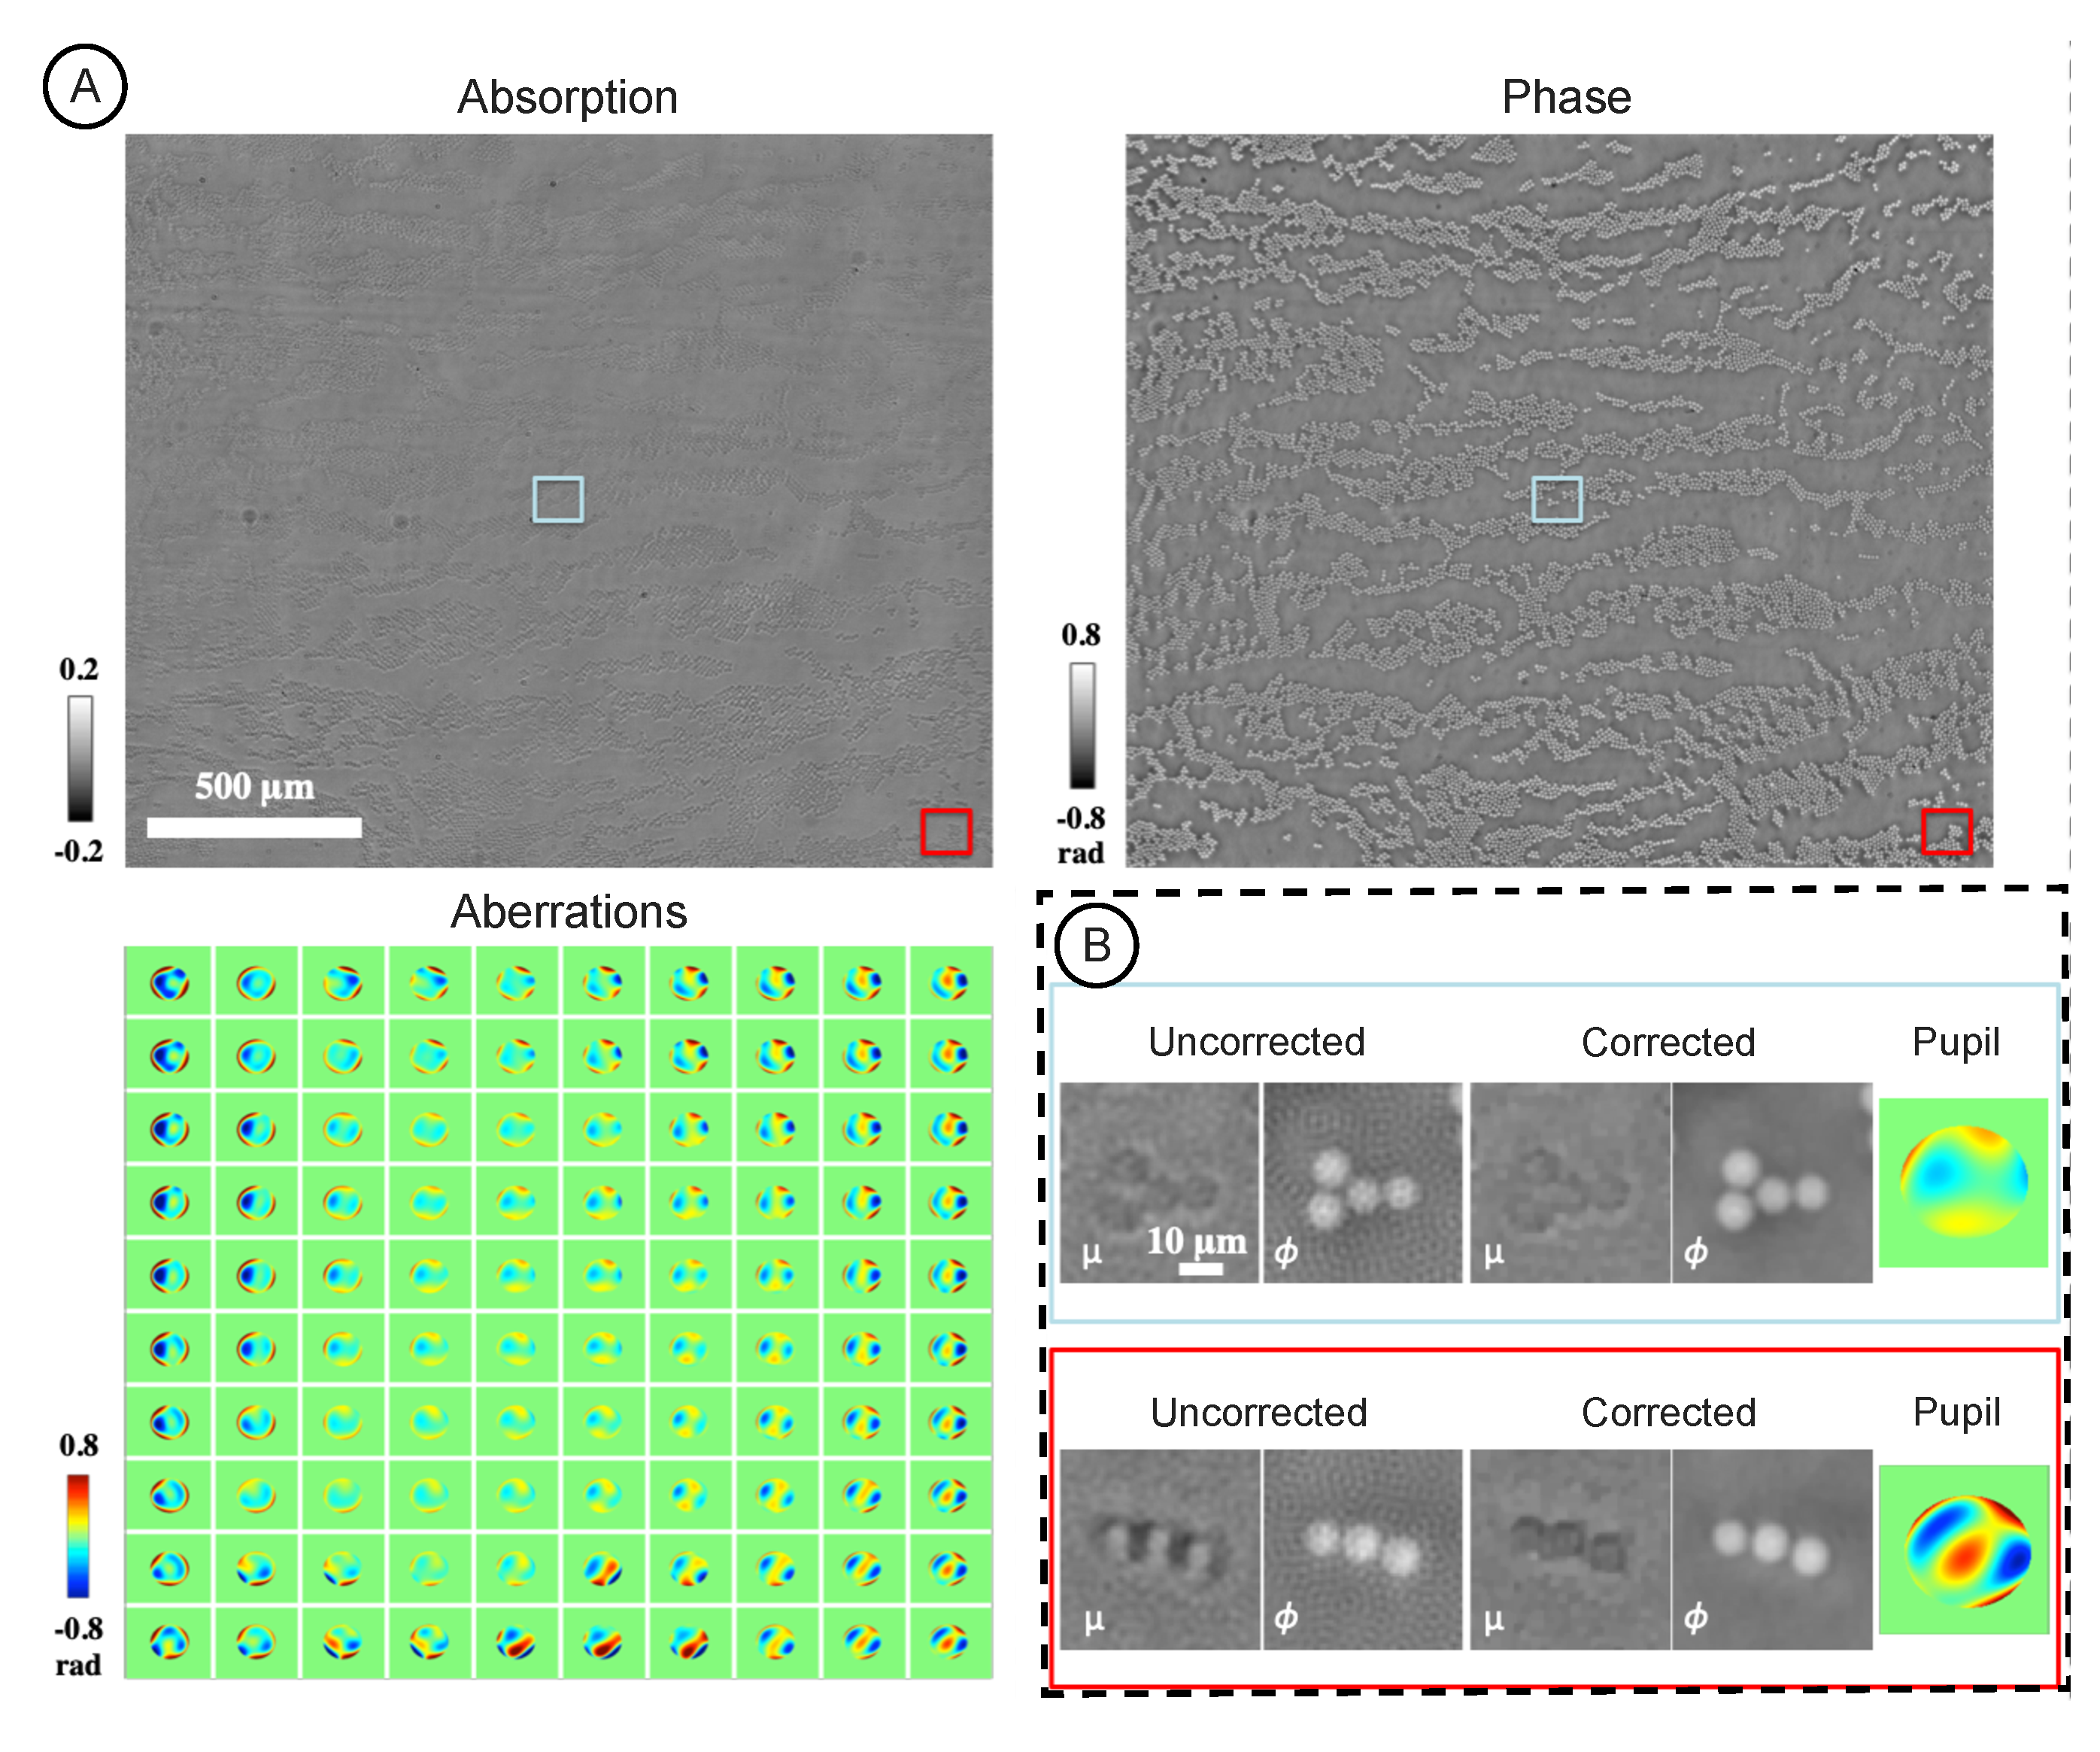
\includegraphics[width=0.9\textwidth]{fig_self_cal_dpc_results3.pdf}
\caption{\label{fig:self_cal_dpc_experimentalresults3} (a) Reconstructed absorption, phase and spatially-varying aberrations (recovered pupil wavefronts for different regions of the field-of-view). (b) Comparison of results with and without pupil estimation for central and edge regions of the field-of-view.}
\end{figure}

In computational imaging systems, system aberrations can significantly degrade quantitative phase and absorption reconstructions if not properly compensated. In order to correct the aberration without conducting additional measurements to calibrate the system, joint estimation of the sample and the pupil function is needed. While Fourier ptychography or coded aperture imaging provides pupil recovery, these methods often require many measurements. In this paper, we demonstrated a DPC-based phase retrieval technique that simultaneously recovers the system pupil function and quantitative phase and absorption of a sample with only 4 intensity images. By combining 3 DPC images as well as 1 measurement made under coherent illumination, diffraction-limited field and aberration with arbitrary Zernike orders were acquired through an alternating non-convex optimization. This method not only reduces the data acquisition time, but also increases signal-to-noise ratio due to higher light throughput compared to single-LED acquisition. The recovered system aberration are general to the system, and may be used for image correction in other imaging modalities, such as deconvolution of fluorescence images~\cite{Chung2016}.

\section{Source Self-Calibration using Fourier Ptychography}\label{sec:selfcal:fpm}

Computational imaging leverages the power of both optical hardware and computational algorithms to reconstruct images from indirect measurements. In optical microscopy, programmable sources have been used for computational illumination techniques including multi-contrast~\cite{Zheng2011,Liu2014}, quantitative phase~\cite{Zheng2013,Tian14,tian2015quantitative,Chen2016} and super-resolution~\cite{Zheng2013,ou2013quantitative,Dong:14,Tian2014}. Implementation is simple, requiring only an inexpensive source attachment for a commercial microscope. However, these methods are also sensitive to experimental misalignment errors and can suffer severe artifacts due to model mismatch. Extensive system calibration is needed to ensure that the inverse algorithm is consistent with the experimental setup, which can be time- and labor-intensive. This often requires significant user expertise, making the setup less accessible to reproduction by non-experts and undermining the simplicity of the scheme. Further, pre-calibration methods are not robust to changes in the system (e.g. bumping the setup, changing objectives, sample-induced aberrations) and require precise knowledge of a ground-truth test object.

Algorithmic self-calibration methods ~\cite{Thibault2009,Ou:14,Horstmeyer:14,Yeh2015,Sun:16LEDpos,Liu:17, maiden2012annealing, zhang2013translation,Bian:13,Bian:16,Dou2017,Eckert:16,Satat2016,Pan2017,Chung:16fluor} eliminate the need for pre-calibration and precise test objects by making calibration part of the inverse problem. These methods jointly solve two inverse problems: one for the reconstructed image of the object and the other for the calibration parameters. By recovering system calibration information directly from captured data, the system becomes robust to dynamic changes in the system.

\begin{figure*}[t]
	\centering
	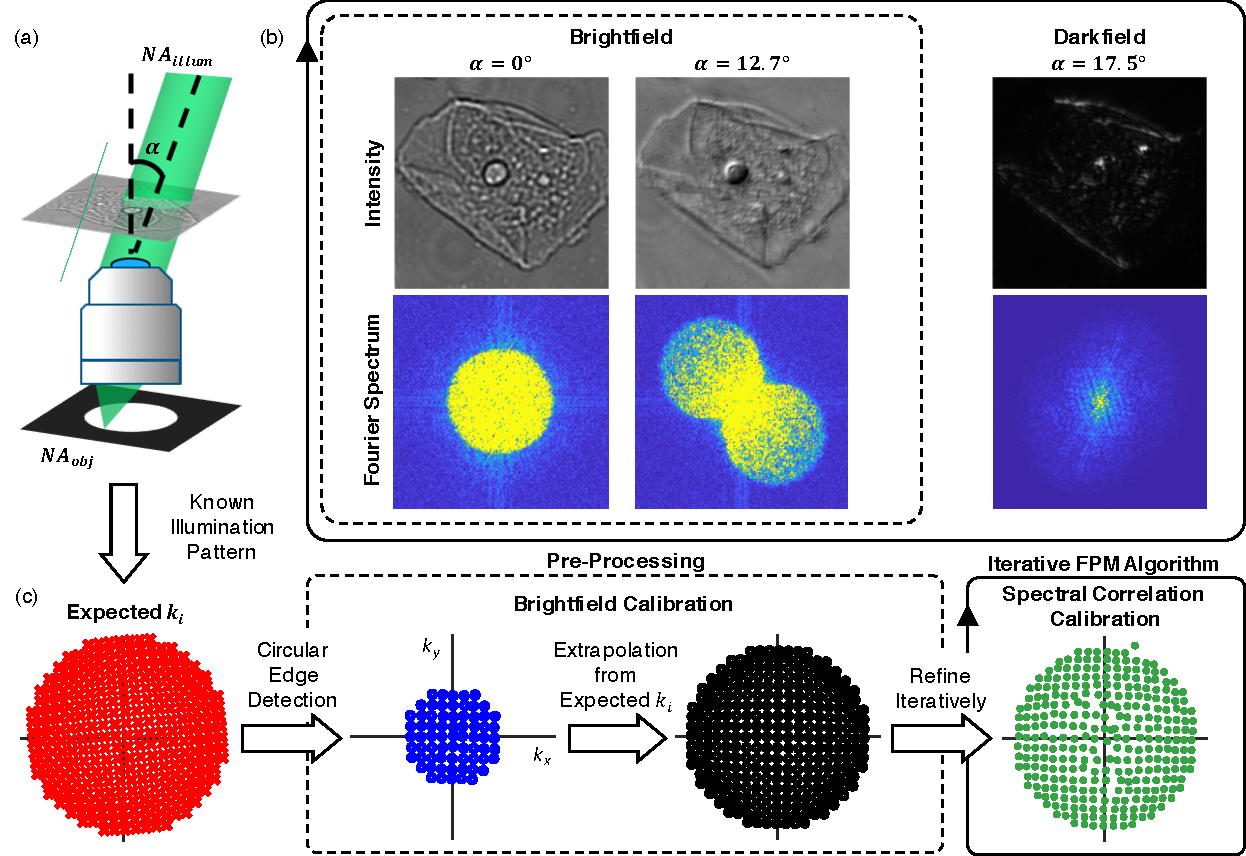
\includegraphics[width=0.85\textwidth]{figures/fig_selfcal_fpm_overview.pdf}
	\caption{Illumination angles are calibrated by analyzing Fourier spectra. (a) A cheek cell is illuminated at angle $\alpha$ and imaged with $NA_{obj}$. (b) Brightfield images contain overlapping circles in their Fourier spectra; darkfield images do not. (c) We perform a fast and efficient brightfield calibration in pre-processing, then extrapolate the correction to darkfield images and, finally, iteratively calibrate angles inside the FPM algorithm using a spectral correlation calibration.
		}
	\label{fig:self_cal_fpm_overview}
\end{figure*}

Here, we focus on \textit{illumination angle} self-calibration for Fourier Ptychographic Microscopy (FPM)~\cite{Zheng2013}. FPM is a coherent computational imaging method that reconstructs high-resolution amplitude and phase across a wide field-of-view (FOV) from intensity images captured with a low-resolution objective lens and a dynamically-coded illumination source. Images captured with different illumination angles are combined computationally in an iterative phase retrieval algorithm that constrains the measured intensity in the image domain and pupil support in the Fourier domain. This algorithm can be described as stitching together different sections of Fourier space (synthetic aperture imaging~\cite{Turpin:1995,Di:08}) coupled with iterative phase retrieval. FPM has enabled fast \textit{in vitro} capture via multiplexing~\cite{Tian2014,tian2015quantitative}, fluorescence imaging~\cite{Chung:16fluor}, and 3D microscopy~\cite{tian20153d,Horstmeyer:16}. It requires significant redundancy (pupil overlap) in the dataset~\cite{Dong:14,Sun:16}, making it suitable for joint estimation self-calibration.

Self-calibration routines have previously been developed to solve for pupil aberrations~\cite{Thibault2009,Ou:14,Horstmeyer:14}, illumination angles~\cite{Yeh2015,Sun:16LEDpos,Liu:17, maiden2012annealing, zhang2013translation}, LED intensity~\cite{Bian:13}, sample motion~\cite{Bian:16}, and auto-focusing~\cite{Dou2017} in FPM. The state-of-the-art self-calibration method for illumination angles is simulated annealing~\cite{Yeh2015,Sun:16LEDpos}, a joint estimation solution which (under proper initialization) removes LED misalignment artifacts that usually manifest as low-frequency noise. Unfortunately, because the simulated annealing procedure operates inside the FPM algorithm iterative loop, it slows the run-time of the solver by an order of magnitude or more. For 3D FPM (which is particularly sensitive to angle calibration~\cite{tian20153d}), the computational costs become infeasible.

Moreover, most self-calibration algorithms require a relatively close initial guess for the calibration parameters. This is especially true when the problem is non-convex or if multiple calibration variables are to be solved for (\textit{e.g.} object, pupil, and angles of illumination). Of the relevant calibration variables for FPM, illumination angles are the most prone to error, due to shifts or rotations of the LED array~\cite{Guo:15}, source instabilities~\cite{Kuang:15,Eckert:16}, non-planar illuminator arrangements~\cite{Chung2016,phillips2015multi,Sen:16,Phillips:17}, or sample-induced aberrations~\cite{Hell:1993,Kang:18}. Sample-induced aberrations can also change the effective illumination angles dynamically, such as when the sample is in a moving aqueous solution.

We propose here a two-pronged angle self-calibration method that uses both pre-processing (\textit{brightfield calibration}) and iterative joint estimation (\textit{spectral correlation calibration}) that is quicker and more robust to system changes than state-of-the-art calibration methods\footnote{This work was developed in close collaboration with fellow Ph.D. student Regina Eckert (Waller Lab, EECS, UC Berkeley)}. A circle-finding step prior to the FPM solver accurately identifies the angles of illumination in the brightfield (BF) region. A transformation between the expected and BF calibrated angles extrapolates the correction to illuminations in the darkfield (DF) region. Then, a local grid-search-based algorithm inside the FPM solver further refines the angle estimates, with an optional prior based on the illuminator geometry (Fig.~\ref{fig:self_cal_fpm_overview}). Our method is object-independent, robust to coherent noise, and time-efficient, adding only seconds to the processing time. We demonstrate on-line angle calibration for 2D and 3D FPM with 3 different source types: an LED array, a galvanometer-steered laser, and a high-NA (max $NA_{illum} = 0.98$) quasi-dome illuminator~\cite{Phillips:17}.

\subsection{Methods}
The image formation process for a thin sample under off-axis spatially coherent plane wave illumination can be described by:
\begin{equation}
\vec{I}_i(\vec{r}) = |\vec{O}(\vec{r})e^{-i2\pi \vec{k}_i\vec{r}} * \vec{P}(\vec{r})|^2 = |\mat{F}^{-1}(\tilde{\vec{O}}(\vec{k}-\vec{k}_i)\tilde{\vec{P}}(\vec{k}))|^2,
\label{eq:forwardModel}
\end{equation}

\noindent where $\vec{k}_i$ is the spatial frequency of the incident light, $\tilde{\vec{P}}(\vec{k})$ is the system pupil function, $\tilde{\vec{O}}(\vec{k})$ is the object Fourier spectrum, and $\mat{F}$ is the 2D Fourier transformation operation, valid for shift-invariant systems. Intensity images are captured at the sensor plane, corresponding to auto-correlation in the Fourier domain:

\begin{equation}
\begin{split}
\tilde{\vec{I}}_i(\vec{k}) &= \mat{F}(|\vec{O}(\vec{r})e^{-i2\pi \vec{k}_i\vec{r}} * \vec{P}(\vec{r})|^2) \\
&=\tilde{\vec{O}}(\vec{k}-\vec{k}_i)\tilde{\vec{P}}(\vec{k}) \star \tilde{\vec{O}}(\vec{k}-\vec{k}_i)\tilde{\vec{P}}(\vec{k}),
\end{split}
\label{eq:Fourier domain}
\end{equation}

\noindent where $*$ denotes convolution and $\star$ denotes auto-correlation. $\tilde{\vec{O}}(\vec{k}-\vec{k}_i)\tilde{\vec{P}}(\vec{k})$ corresponds to the shifted spectrum of the object within the circle $|\vec{k}| \leq \frac{NA_{obj}}{\lambda}$ and 0 everywhere else. The auto-correlation operation essentially scans two copies of $\tilde{\vec{O}}(\vec{k}-\vec{k}_i)\tilde{\vec{P}}(\vec{k})$ across each other, coherently summing at each shift to give $\tilde{\vec{I}}_i(\vec{k})$. Typically, the object spectrum has a large zero-order (DC) term that decays sharply towards higher frequencies. In the brightfield region, when the DC term at $\vec{k}_i$ is within the pupil's passband, the auto-correlation effectively scans this DC term across the conjugate spectrum, giving high values where the DC term overlaps with the conjugate pupil and negligible signal elsewhere. This interference between the DC term and pupil in the auto-correlation creates two distinct circles centered at $\vec{k}_i$ and $-\vec{k}_i$ in the intensity spectrum amplitude (Fig.~\ref{fig:self_cal_fpm_overview}). Hence, we can calibrate the illumination angle by finding these circle centers. For darkfield images, the DC term is outside $\frac{NA_{obj}}{\lambda}$ and so we do not observe clearly defined circles in $|\tilde{\vec{I}}_i|$ (Fig.\ref{fig:self_cal_fpm_overview}b), making calibration more complicated.

Our algorithm relies on analysis of the raw intensity Fourier transform to recover illumination angles. Fourier domain analysis of intensity images has been used previously to deduce aberrations~\cite{Shanker:16} and determine the center of diffraction patterns~\cite{DAMMER1997214,CAUCHIE2008567} for system calibration. We show here that the individual Fourier spectra can be used to accurately determine illumination angles in both the brightfield and darkfield regime.

\subsection{Brightfield Calibration}
Locating the center of the circles in the amplitude of a Fourier spectrum is an image processing problem. Previous work in finding circles in images uses the Hough transform, which relies on an accurate edge detector as an initial step~\cite{Yuen89,Davies:04}. In practice, however, we find that edge detectors do not function well on our datasets due to speckle noise, making the Hough transform an unreliable tool for our purpose.

\begin{figure} [tb]
	\centering
	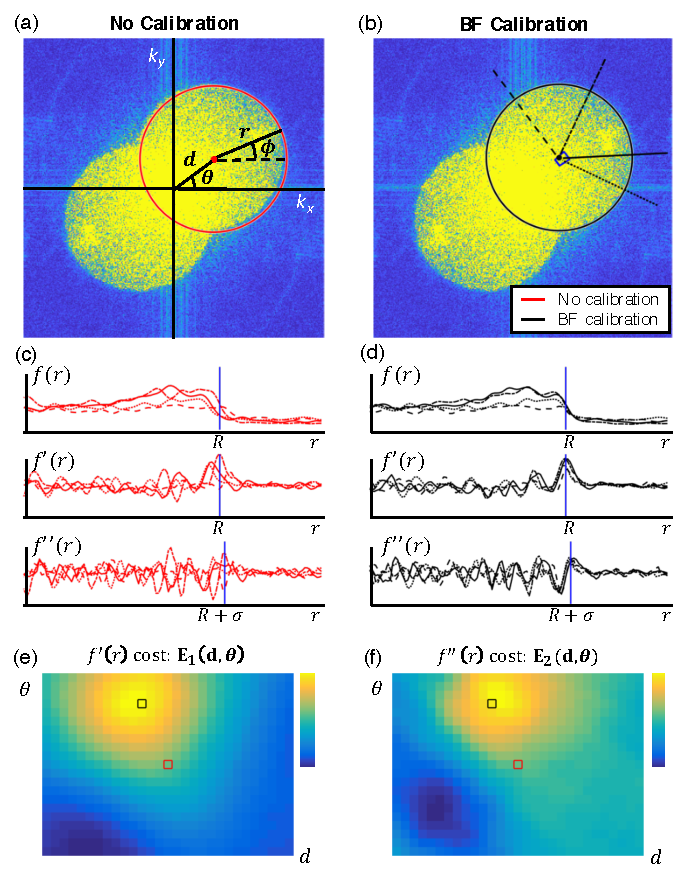
\includegraphics[width=0.6\textwidth]{figures/fig_selfcal_fpm_bf.pdf}
	\caption{Circular edge detection on brightfield images finds circle centers, giving illumination angle calibration. (a,b) Comparison of uncalibrated (red) and calibrated (black) illumination $\vec{k}_i$. The blue box in (b) indicates the search range for $\vec{k}_i$. (c,d) $\tilde{\vec{I}_i}$ along radial lines, $f(r,\phi_n)$, and derivatives with respect to $r$. (e,f) $\vec{E}_1$ and $\vec{E}_2$, sums of the derivatives at known radii $R$ and $R+\sigma$, peak near the correct center. Boxes show uncalibrated (red) and calibrated (black) $\vec{k}_i$ centers.
		}
	\label{fig:BF_calibration}
\end{figure}

Intuitively, circular edge detection can be understood as performing edge detection (\textit{i.e.} calculating image gradients) along a circular arc around a candidate center point in k-space (the Fourier domain). To first approximation, we assume $|\tilde{\vec{I}_i}|$ is a binary function that is 1 inside the two circles and 0 everywhere else. Our goal is to find the strong binary edge in order to locate the circle center.  We need only consider one of the circles, since the intensity image is real-valued and so its Fourier transform is symmetric. Based on information we have about our illumination set-up, we \textit{expect} the illumination spatial frequency (and therefore circle center) for spectrum $\tilde{\vec{I}_i}$ to be at $\vec{k}_{i,0} = (k_{x,i,0},k_{y,i,0})$ (polar coordinates $\vec{k}_{i,0} = (d_{i,0}, \theta_{i,0})$) (Fig.~\ref{fig:BF_calibration}a). If this is the \textit{correct} center  $\vec{k}_i'$, we expect there to be a sharp drop in $|\tilde{\vec{I}_i}|$ at radius $R$ along any radial line $f(r,\phi_n)$ out from $\vec{k}_i'$ (Fig.~\ref{fig:BF_calibration}b). This amplitude edge will appear as a peak at $r=R$ in the first derivative of each radial line with respect to $r$, $f'(r,\phi_n)$ (Fig.~\ref{fig:BF_calibration}d). Here $(r,\phi_n)$ are the polar coordinates of the radial line with respect to the center $\vec{k}_i$, considering the $n^{th}$ of $N$ radial lines.

We identify the correct $\vec{k}_i'$ by evaluating the summation of the first derivative around the circular arc at $r=R$ from several candidate $\vec{k}_i = (d_i,\theta_i)$ positions:

\begin{equation}
\vec{E}_1(R, d_i,\theta_i)=\sum_{n=1}^{N} f'(r = R,\phi_n,d_i,\theta_i).
\label{eq:eprime}
\end{equation}

\noindent When $\vec{k}_i$ is incorrect, the edges do not align and the derivative peaks do not add constructively at $R$ (Fig.~\ref{fig:BF_calibration}c). The derivatives at $R$ are all maximized \textit{only} at the correct center $\vec{k}_i'$ (Fig.~\ref{fig:BF_calibration}d), creating a peak in $\vec{E}_1$ (Fig.~\ref{fig:BF_calibration}e). This is analogous to applying a classic edge filter in the radial direction from a candidate center and accumulating the gradient values at radius $R$.

In order to bring our data closer to our binary image approximation, we divide out the average spectrum $\mathrm{mean}_i(|\tilde{\vec{I}_i}|)$ across all $i$ spectra. Because the object remains constant across images while the angles of illumination change, the average spectrum is similar in form to the object's auto-correlation spectrum, with a sharp central peak decaying towards higher frequencies. The resulting normalized spectra contain near-constant circles on top of background from higher-order terms. We then convolve with a Gaussian blur kernel with standard deviation $\sigma$ to remove speckle noise (Alg.~\ref{alg:BF}.\ref{alg:1}-\ref{alg:2}). Experi

mentally, we choose $\sigma = 2$ pixels, which balances blurring speckle noise and maintaining the circular edge. Under this model, the radial line $f(r,\phi_n)$ from our correct center $\vec{k}_i'$ can be modeled near the circular edge as a binary step function convolved with a Gaussian:

\begin{equation}
f(r,\phi_n,d_i',\theta_i') = \text{rect}(\frac{r}{2R}) * \frac{1}{\sqrt{2\pi}\sigma}e^{\frac{-r^2}{2\sigma^2}}.
\label{eq:spoke}
\end{equation}


\noindent By differentiating through $f'''(r,\phi_n)$ and setting equal to zero, we find the peak of $f'(r,\phi_n)$ still occurs at $r=R$. Additionally, we find that the second derivative $f''(r,\phi_n)$ has a maximum at $r=R+\sigma$. Experimentally, we have found that considering both the first \textit{and} second derivatives increases our accuracy and robustness to noise across a wide variety of datasets. We therefore calculate a second derivative metric,

\begin{equation}
\vec{E}_2(R+\sigma,d_i,\theta_i)=\sum_{n=1}^{N} f''(r = R+\sigma,\phi_n,d_i,\theta_i),
\label{eq:edoubleprime}
\end{equation}

\noindent which is jointly considered with Eq.~\ref{eq:eprime}. We identify candidate centers $\vec{k}_i$ that occur near the peak of \textit{both} $\vec{E}_1$ and $\vec{E}_2$ (Fig.~\ref{fig:BF_calibration}e-f), then use a least-squares error metric to determine the final calibrated $\vec{k}_i'$ (Alg.~\ref{alg:BF}.\ref{alg:5}-\ref{alg:8}). In practice, we also only consider the non-overlapping portion of the circle's edge, bounding $\vec{\phi}$.

Until now, we have assumed that the precise radius $R$ of the pupil is known. However, in pixel units, $R$ is dependent on the pixel size of the sensor, $p_s$, and the system magnification, $mag$:

\begin{equation}
R = \frac{NA_{obj}}{\lambda} \frac{p_s*M}{mag},
\end{equation}

\noindent as well as $NA_{obj}$ and $\lambda$, where $\tilde{\vec{I}_i}$ is dimension $M\times M$. Given that $mag$ and $NA_{obj}$ are often imprecisely known but are unchanged across all images, we calibrate the radius by finding the $R'$ which gives the maximum gradient peak $\vec{E}_1$ across multiple images before calibrating $\vec{k}_i'$ (Alg.~\ref{alg:BF}.\ref{alg:3}). A random subset of images may be used to decrease computation time.

\begin{algorithm}
\caption{Brightfield Calibration}\label{alg:BF}
\begin{algorithmic}[1]
\State $\tilde{\vec{I}}_f \gets |\tilde{\vec{I}}|/\textrm{mean}_i(|\tilde{\vec{I}_i}|)$\Comment{Divide out mean spectrum}\label{alg:1}
\State $\tilde{\vec{I}}_f \gets \textrm{gauss}(\tilde{\vec{I}}_f,\sigma)$\Comment{Smooth speckle}\label{alg:2}
\State $R' \gets \argmax_R \vec{E}_1(R,d_i,\theta_i), \textrm{subset }(\tilde{\vec{I}}_{f,i})$\Comment{Calibrate radius}\label{alg:3}
\For{$i^{th}$ image}
\Comment{Circular edge detection}
\State $\vec{k}_{i,1} \gets (d_i,\theta_i) \textrm{ where } \vec{E}_1 \textrm{ near max (within 0.1 std)}$\label{alg:5}
\State $\vec{k}_{i,2} \gets (d_i,\theta_i) \textrm{ where } \vec{E}_2 \textrm{ near max}$
\State $\vec{k}_{i} \gets \vec{k}_{i,1} \cap \vec{k}_{i,2}$\Comment{Consider both metrics}
\State $\vec{k}_i' \gets \argmin_{\vec{k}_i} ||\vec{I}_i - \mat{F}(\tilde{\vec{I}_i}\cdot\tilde{\vec{P}}(\vec{k}-\vec{k_i}))||_2$ \Comment{Evaluate $\vec{k}_i$}
\EndFor \label{alg:8}
\State $\mat{A}, i_{outliers} \gets \textrm{RANSAC}(\mat{A}=\vec{k}_i'/\vec{k}_{i,0})$\Comment{Identify outliers} \label{alg:9}
\State $\vec{k}_{inliers}^{(0)} \gets \vec{k}_{inliers}'$\Comment{Initialize for FPM}
\State $\vec{k}_{outliers}^{(0)} \gets \mat{A}\vec{k}_{outliers,0}$
\State $\vec{k}_{darkfield}^{(0)} \gets \mat{A}\vec{k}_{darkfield,0}$ \label{alg:12}

\end{algorithmic}
\end{algorithm}

\subsection{Spectral Correlation Calibration}
While the brightfield (BF) calibration method localizes illumination angles using intrinsic contrast from each measurement, this contrast is not present in high-angle (darkfield) measurements (Fig.~\ref{fig:self_cal_fpm_overview}b). Therefore, we additionally solve a more general joint estimation problem to refine the initialization provided by BF calibration, where the object $\vec{O}(\vec{r})$, pupil $\vec{P}(\vec{k})$, and illumination angles $\vec{k_i}$ are optimized within the FPM algorithm. At each inner iteration, we estimate the $i^{th}$ illumination angle by minimizing the FPM objective function with respect to illumination angle (Fig.~\ref{fig:DF_calibration}a). This step finds the relative k-space location of the current spectrum $\tilde{\vec{I}_i}$ relative to the overall object, providing an estimate $\vec{k}_i^{(m)}$ relative to the other illuminator angles $\vec{k}^{(m)}_j$, $j\neq i$. We call this the spectral correlation method because this optimization implicitly finds $\vec{k}_i^{(m)}$ which best aligns the $i^{th}$ spectrum with the estimated object spectrum $\tilde{\vec{O}}(\vec{k})^{(m)}$.

\begin{figure*}[hbt]
	\centering
	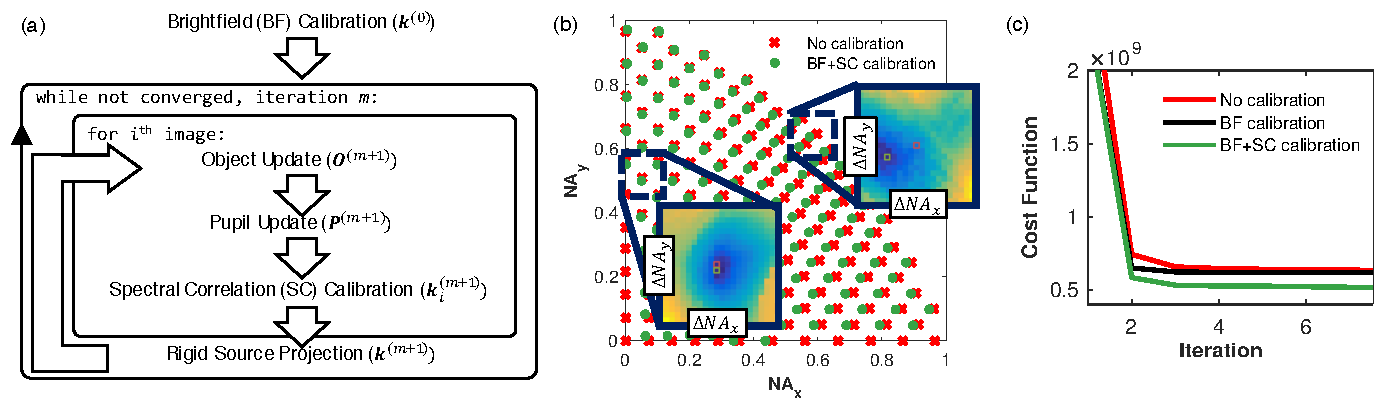
\includegraphics[width=0.97\textwidth]{figures/fig_selfcal_fpm_df.pdf}
	\caption{BF calibration uses a fast pre-processing step to estimate illumination angles, then SC calibration iteratively refines them within the FPM solver. (a) Algorithm block diagram, (b) uncalibrated (red) and BF + SC calibrated (green) illumination angle map. Insets are example search spaces, showing local convexity. (d) FPM convergence plot for different methods.
		}
	\label{fig:DF_calibration}
\end{figure*}

Unlike previous joint estimation methods~\cite{Yeh2015,Sun:16LEDpos}, we constrain $\vec{k}_i$ to exist on the k-space grid defined by the our image sampling. Our k-space resolution is band-limited by the size of the image patch, $\vec{s}=(s_x,s_y)$, across which the illumination can be assumed coherent. This coherent area size is determined by the van Cittert-Zernike theorem, which can be simplified~\cite{BornWolf} to show that the coherence length $l_c$ of illumination with mean source wavelength $\bar{\lambda}$ produced by a source of size $\rho$ at a distance $R$ is determined by:

\begin{equation}\label{eq:vancittert_zernike}
l_c = \frac{0.61 R \bar{\lambda}}{\rho}.
\end{equation}

\noindent For example, a $300\mu m$ wide LED placed $50 mm$ above the sample with $\bar{\lambda} = 530nm$ gives $l_c = 53.8\mu m$, which provides an upper bound on the size of image patch used in the FPM reconstruction, $(s_x,s_y) \leq l_c$. This limitation imposes a minimum resolvable discretization of illumination angles $\Delta{\vec{k}} = \frac{2}{\vec{s}}$ due to the Nyquist criterion. Since we cannot resolve finer angle changes, we need only perform a local grid search over integer multiples of $\Delta{\vec{k}}$, which makes our joint estimation SC method much faster than previous methods.

SC calibration is cast as an iterative optimization of discrete perturbations of the estimated angle using a local grid search. At each FPM iteration, we solve for the optimal perturbation of illumination angle  $\vec{{k}}_i^{(m)}$ over integer multiples $\vec{n} = (n_x, n_y)$ of k-space resolution-limited steps $\Delta \vec{k}$ such that the updated illumination position $\vec{k}_i^{(m+1)} = \vec{{k}}_i^{(m)} + \vec{n} \cdot \vec{\Delta {k}}$ minimizes the $\ell 2$ distance between the object and illumination angle estimates and measurements,

\begin{equation}\label{Eq:positionOpt}
    \begin{aligned}
    & \underset{\vec{n}}{\text{argmin}}
    & & ||\vec{I}_{i}- |\vec{O}^{(m+1)} e^{-i2\pi (\vec{{k}}_i^{(m)} + \vec{n} \Delta\vec{{k}})\vec{\vec{r}}} * \vec{P}^{(m+1)}|^2||_2^2 \\
    & \text{subject to}
    & &  \vec{n} = (n_x, n_y), \qquad (n_x, n_y) \in [-1, 0 ,1].
    \end{aligned}
\end{equation}

\noindent This grid search is performed iteratively within each sequential iteration of an FPM reconstruction until $\vec{k}_i$ converges, giving a lower reconstruction cost than BF calibration alone (Fig.~\ref{fig:DF_calibration}b-c).

The choice of $\vec{n} = (n_x, n_y)$ to search can be tuned to match the problem. In most experimental cases, we find that a search of the immediate locality of the current estimate ($(n_x, n_y) \in [-1, 0 ,1]$) gives a good balance between speed and gradient performance when paired with the close initialization from our BF calibration. A larger search range (e.g. $(n_x, n_y) \in [-2, -1, 0, 1, 2]$) may be required in the presence of noise or without a close initialization, but the number of points searched will increase with the square of the search range, causing the algorithm to slow considerably.



\begin{figure*} [htb]
	\centering
	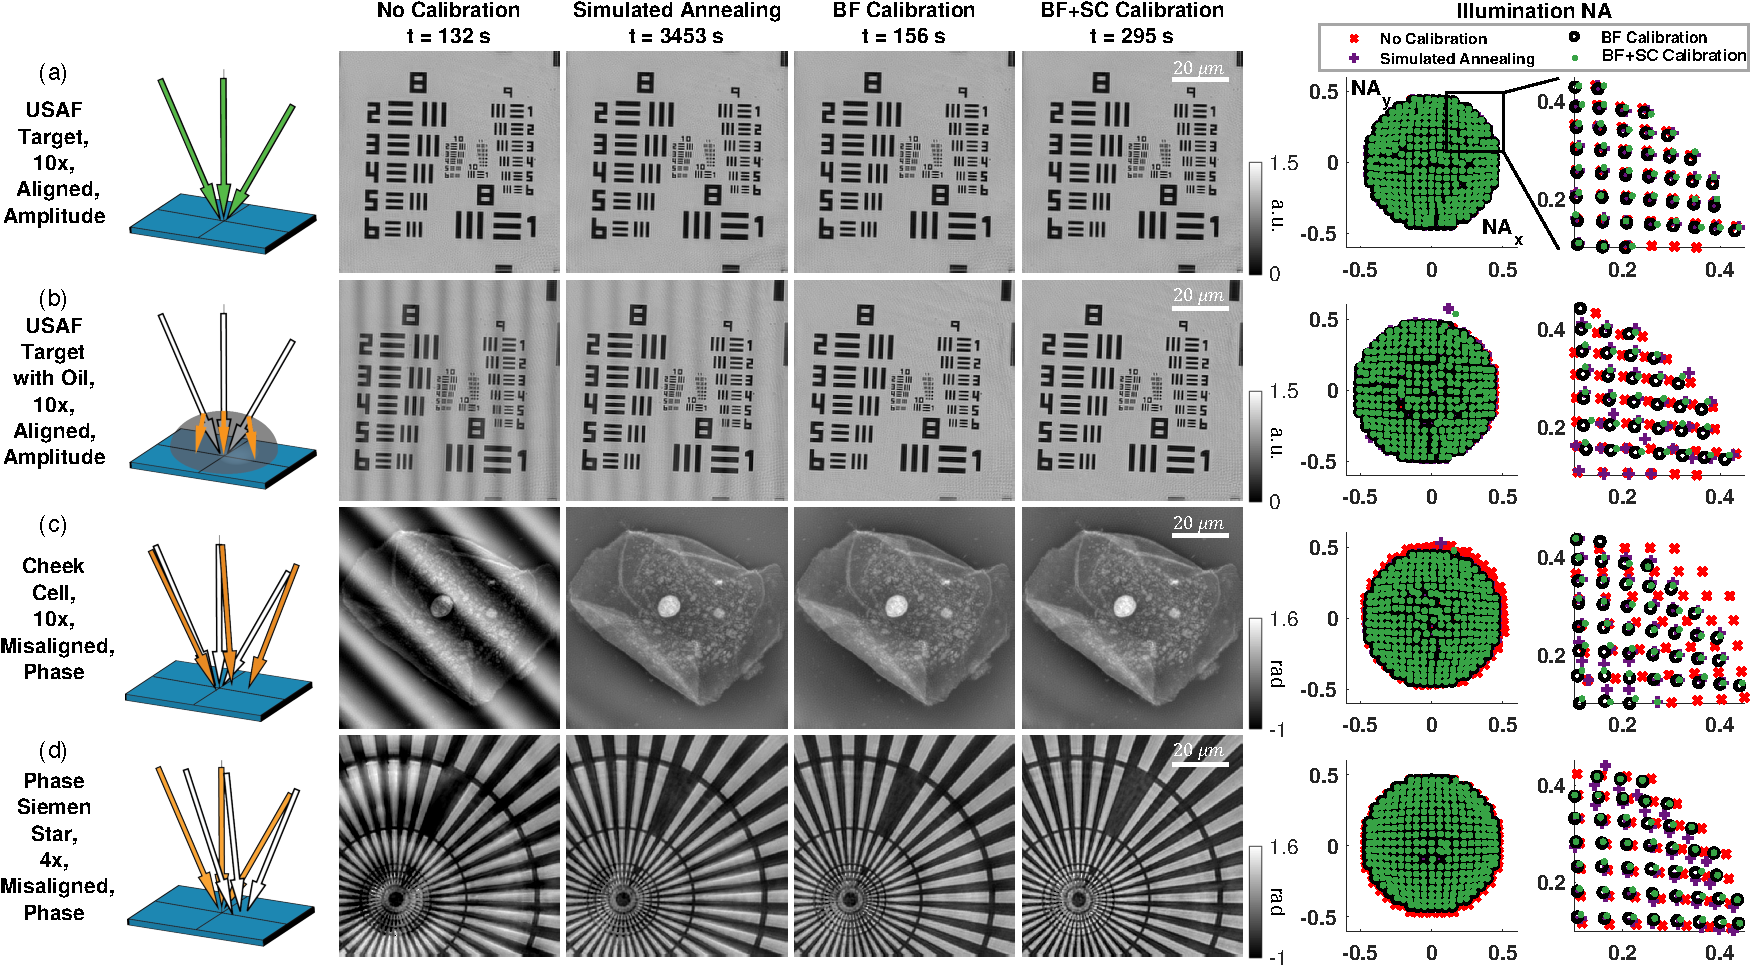
\includegraphics[width=1\textwidth]{figures/fig_selfcal_fpm_mosaic.pdf}
	\caption{Experimental results with an LED array microscope, comparing reconstructions with no calibration (average reconstruction time 132 seconds), simulated annealing (3453 s), our BF calibration (156 s), and our BF + SC calibration (295 s). (a) Amplitude reconstructions of a USAF target in a well-aligned system. (b) Amplitude reconstructions of the same USAF target with a drop of oil placed on top of the sample to simulate sample-induced aberrations. (c) Phase reconstructions of a human cheek cell with computationally misaligned illumination, and (d) a Siemens star phase target with experimentally misaligned illumination.
		}
	\label{Fig:results}
\end{figure*}



Including prior information about the design of the illumination source can make our calibration problem more well-posed. For example, we can include knowledge that an LED array is a rigid, planar illuminator in our initial guess of the illumination angle map, $\vec{k}_{i,0}$. By forcing the current estimates $\vec{k}_i^{(m)}$ to fit a transformation of this initial angle map at the end of each FPM sub-iteration, we can use this knowledge to regularize our optimization (Fig.~\ref{fig:DF_calibration}a). The transformation model used depends on the specific illuminator. For example, our quasi-dome LED array is composed of five circuit boards with precise LED positioning within each board but variable board position relative to each other. Thus, imposing an affine transformation from the angle map of each board to the current estimates $\vec{k}_i^{(m)}$ significantly reduces the problem dimensionality and mitigates noise across LEDs, making the reconstruction more stable.

\subsection{Results}

\begin{figure*} [t]
	\centering
	\includegraphics[width=1\textwidth]{figures/fig_selfcal_fpm_system.pdf}
	\caption{Experimental angle calibration in laser and high-NA quasi-dome illumination systems. (a) Laser illumination is steered by a dual-axis galvanometer. The angled beam is relayed to the sample by 4", 80 mm focal length lenses. (b) Our calibration method removes low-frequency reconstruction artifacts. (c) The quasi-dome illuminator enables up to 0.98 $NA_{illum}$ using programmable LEDs. (d) Our 1.23 NA reconstruction provides isotropic 425 $nm$ resolution with BF + SC calibration.
		}
	\label{Fig:laserDome}
\end{figure*}

\subsubsection{Planar LED Array}
We first show experimental results from a conventional LED array illumination system with a 10$\times$, 0.25 NA and a 4$\times$, 0.1 NA objective lens at $\lambda = 514 nm$ and $NA_{illum} \leq 0.455$ (Fig.~\ref{Fig:results}). We compare reconstructions with simulated annealing, our BF pre-processing alone, and our combined BF+SC calibration method. All methods were run in conjunction with EPRY pupil reconstruction~\cite{Ou:14}. We include results with and without the SC calibration to illustrate that the BF calibration is sufficient to correct for most misalignment of the LED array since we can accurately extrapolate LED positions to the darkfield region when the LEDs fall on a planar grid. However, when using a low NA objective ($NA_{obj} \leq 0.1$), as in Fig.~\ref{Fig:results}d, the SC method becomes necessary because the BF calibration is only able to use 9 images (compared to 69 brightfield images with a 10$\times$, 0.25 NA objective, as in Fig.~\ref{Fig:results}a-c).

Our method is object-independent, so can be used for phase and amplitude targets as well as biological samples. All methods reconstruct similar quality results for the well-aligned LED array with the USAF resolution target (Fig.~\ref{Fig:results}a). To simulate an aqueous sample, we place a drop of oil on top of the resolution target. The drop causes uneven changes in the illumination, giving low-frequency artifacts in the uncalibrated and simulated annealing cases which are corrected by our method (Fig.~\ref{Fig:results}b). Our method is also able to recover a $5^{\circ}$ rotation, 0.02 NA shift, and 1.1$\times$ scaled computationally-imposed misalignment on well-aligned LED array data for a cheek cell (Fig.~\ref{Fig:results}c), and gives a good reconstruction of an experimentally misaligned LED array for a phase Siemens star (Benchmark Technologies, Inc.) (Fig.~\ref{Fig:results}d). In contrast to simulated annealing, which on average takes $26 \times$ as long to process as FPM without calibration, our brightfield calibration only takes an additional 24 seconds of processing time and the combined calibration takes roughly only $2.25 \times$ as long as no calibration.

\subsubsection{Steered Laser}
Laser illumination can be used instead of LED arrays to increase the coherence and light efficiency of FPM~\cite{Kuang:15,Chung2016}. In practice, laser systems are typically less rigidly aligned than LED arrays, making them more difficult to calibrate. To verify the performance of our method, we constructed a laser-based FPM system using a dual-axis galvanometer to steer a 532 $nm$, 5 mW laser, which is focused on the sample by large condenser lenses (Fig.~\ref{Fig:laserDome}a). This laser illumination system allows finer, more agile illumination control than an LED array, as well as higher light throughput. However, the laser illumination angle varies from the expected value due to offsets in the dual-axis galvonometer mirrors, relay lens aberrations, and mirror position mis-estimations when run at high speeds. Our method can correct for these problems in a fraction of the time of previous methods (Fig.~\ref{Fig:laserDome}b).

\subsubsection{Quasi-Dome}

Since the FPM resolution limit is set by $NA_{obj} + NA_{illum}$, high-NA illuminators are needed for large space-bandwidth product imaging~\cite{Sun2017,Phillips:17}. To achieve high-angle illumination with sufficient signal-to-noise ratio in the darkfield region, the illuminators must become more dome-like, rather than planar~\cite{phillips2015multi}. We previously developed a novel programmable quasi-dome array made of five separate planar LED arrays that can illuminate up to 0.98 NA~\cite{Phillips:17}. This device uses discrete LED control with RGB emitters ($\bar{\lambda}=[475nm, 530nm, 630nm]$) and can be easily attached to most commercial inverted microscopes (Fig.~\ref{Fig:laserDome}c).

As with conventional LED arrays, we assume that the LEDs on each board are rigidly placed as designed. However, each circuit board may have some relative shift, tilt, or rotation since the final mating of the 5 boards is performed by hand. LEDs with high-angle incidence are both harder to calibrate and more likely to suffer from mis-estimation due to the dome geometry, so the theoretical reconstruction NA would be nearly impossible to reach without self-calibration. Using our method, we obtain the theoretical resolution limit available to the quasi-dome (Fig.~\ref{Fig:laserDome}d). The SC calibration is especially important in the quasi-dome case since it usually has many darkfield LEDs.

\subsection{Discussion}
\begin{figure} [t]
	\centering
	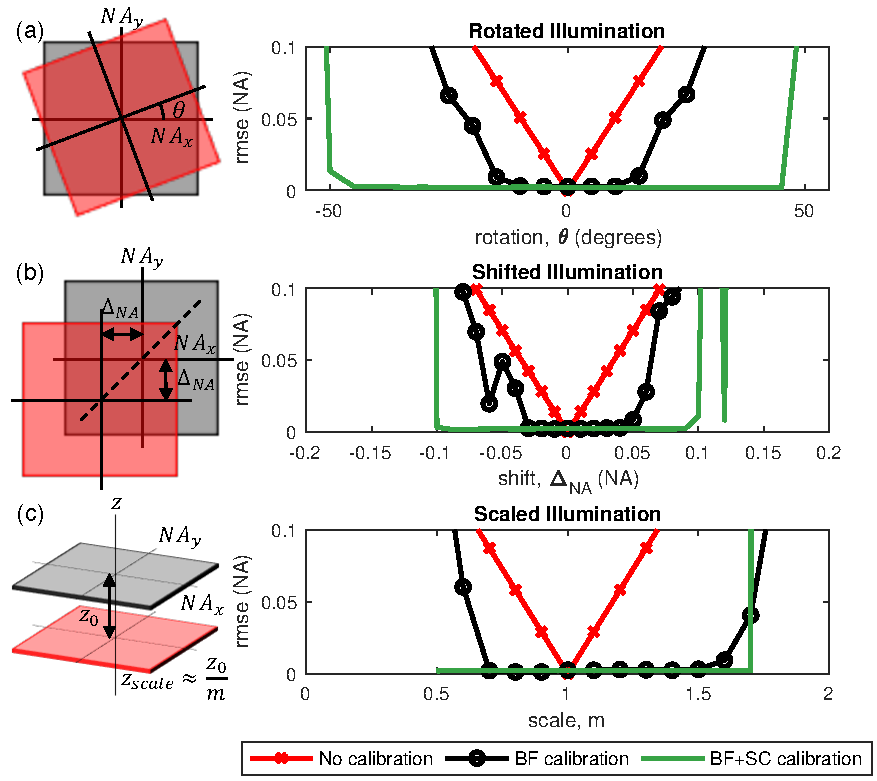
\includegraphics[width=0.5\textwidth]{figures/fig_selfcal_fpm_accuracy.pdf}
	\caption{Our calibration methods are robust to large mismatches between estimated and actual LED array position. Simulation of misaligned illumination by (a) rotation, (b) shift, and (c) scale. Our calibration recovers the illumination with <0.005 NA error for rotations of $-45^{\circ}$ to $45^{\circ}$, shifts of -0.1 to 0.1 NA, and scalings of 0.5$\times$ to 1.75$\times$ before diverging.
		}
	\label{Fig:self_cal_fpm_accuracy}
\end{figure}

Our calibration method offers significant gains in speed and robustness as compared to previous methods. BF calibration enables these capabilities by obtaining a good calibration that needs to be calculated only once in pre-processing, reducing computation. Since an estimation of a global shift in the illuminator based only on the brightfield images provides such a close initialization for the rest of the illumination angles, we can use a quicker, easier joint estimation computation in our SC calibration than would be otherwise possible. Jointly, these two methods work together to create fast and accurate reconstructions.

We analyze the robustness of our method to illumination changes by simulating an object illuminated by a grid of LEDs with $NA_{illum}<0.41$, with LEDs spaced at $0.041 NA$ intervals. We define the system to have $\lambda = 532 nm$, with a 10$\times$, 0.25 NA objective, a 2$\times$ system magnification, and a camera with $6.5 {\mu}m$ pixels. While the actual illumination angles in the simulated data remain fixed, we perturb the expected angle of illumination in typical misalignment patterns for LED arrays: rotation, shift, and scale (analogous to LED array distance from sample). We then calibrate the unperturbed data with the perturbed expected angles of illumination as our initial guess.

Our method recovers the actual illumination angles with error less than 0.005 NA for rotations of $-45^{\circ}$ to $45^{\circ}$ (Fig.~\ref{Fig:self_cal_fpm_accuracy}a); shifts of -0.1 to 0.1 NA, or approximately a displacement of +/- 2 LEDs (Fig.~\ref{Fig:self_cal_fpm_accuracy}b); and scalings of 0.5$\times$ to 1.75$\times$ (or LED array height between 40-140 $cm$ if the actual LED array height is 70 $cm$) (Fig.~\ref{Fig:self_cal_fpm_accuracy}c). In these ranges, the average error is 0.0024 NA, less than the k-space resolution of 0.0032 NA. Hence, our calibrated angles are very close to the actual angles even when the input expected angles are extremely far off. This result demonstrates that our method is robust to most mis-alignments in the illumination scheme.

In summary, we have presented a novel two-part calibration method for recovering the illumination angles of a computational illumination system for Fourier ptychography. We have demonstrated how this self-calibrating method makes Fourier ptychographic microscopes more robust to system changes and aberrations introduced by the sample. The method also makes it possible to use high-angle illuminators, such as the quasi-dome, and non-rigid illuminators, such as laser-based systems, to their full potential. Our pre-processing brightfield calibration further enables 3D multislice Fourier ptychography to reconstruct high-resolution features across larger volumes than previously possible. These gains were all made with minimal additional computation, especially when compared to current state-of-the-art methods. Efficient self-calibrating methods such as these are important to make computational imaging methods more robust and available for broad use in the future.

\section{Summary}

In computational imaging systems, mis-calibrations can significantly degrade reconstructions if not properly compensated for. Here, we have presented two frameworks for algorithmic self-calibration. In Section~\ref{sec:selfcal:dpc}, we presented a novel method for performing self-calibration of system aberrations using just four measurements - three half-circle (DPC) measurements and one coherent (single-LED) measurement. These four measurements enable the recovery of \textit{both} the compelx field of the object as well as spatially-varinat system aberrations. These aberrations can be acquired quickly and reconstructed using standard reconstruction techniques such as ADMM. In Section~\ref{sec:selfcal:fpm}, we presented a novel method for recovering source illumination angles of planar, quasi-domed, and steered laser sources using an offline (image-based) self-calibration algorithm, which is then refined using an online (FPM-based) self-calibration algorithm. For devices subject to manufacturing variations (such as the quasi-dome), these techniques are absolutely essential for high-resolution FPM reconstructions.

Owing to their non-convex formulations, self-calibration will never be as good as proper physical calibration of the systems, when such calibration is possible. However, when mis-calibration is suspected, these methods will always improve reconstruction quality compared to the uncorrected case, and therefore should be used whenever possible. Practically, the performance Quasi-dome presented in Section~\ref{sec:fabrication:quasidome} is significantly improved using self-calibration due to positioning error between printed circuit boards it is composed of. The open-source code used in these sections is provided in the Appendix~\ref{ch:appendix}, Section~\ref{sec:appendix:opensource}.

\chapter{Conclusion}\label{ch:conclusion}
Driving the performance limits of optical microscopy systems requires a unique blend of both hardware and software innovations. Among a wide variety of techniques for probing a sample, coded illumination using a programmable light source is advantageous due to its simplicity and wide utility for various computational imaging techniques. In this work, we proposed a variety of techniques which take advantage of programmable illumination to enable label-free contrast, quantitative imaging, and high-throughput imaging at relatively low cost and complexity on existing optical systems. We have leveraged novel hardware and computational techniques to push performance boundaries in critical areas, such as label-free imaging and neuropathology. Further, we have put significant effort towards quantifying when computational techniques do not provide benefit, acknowledging limiting cases where conventional methods are still state-of-the-art. Taken together, the methods presented in this work illustrate the capabilities of a computational imaging system, and offer evidence of the impact these systems could have on the broader microscopy community.

\begin{wrapfigure}{R}{15em}
  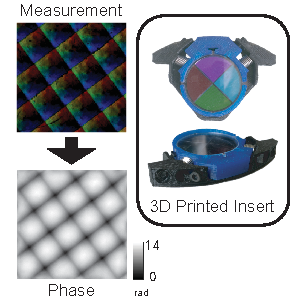
\includegraphics[width=\linewidth]{avatar_phase}
\end{wrapfigure}

In Chapter~\ref{ch:phase} we described differential phase contrast (DPC), a quantitative phase imaging method which uses partially coherent illumination to recover the complex field of a thin (weak) object. We then introduced a single-shot variant of DPC which uses  color-multiplexed illumination to recover the linearized optical field from a single measurement. Our hardware requirements are simple, inexpensive, and compatible with most commercial microscopes through of the use of a color camera and a simple color filter insert placed at the back focal plane of the condenser lens, the same position as many removable phase contrast annulus rings. Unlike phase contrast and DIC, our method does not require special objectives or prisms, which reduces our hardware costs to that of the 3D printed filter itself. In addition, we can use our quantitative phase and amplitude methods to synthesize phase contrast and DIC images digitally, matching the functionality of existing phase imaging systems at a fraction of the cost. Finally, we presented a framework for analyzing the source design for DPC-based system in terms of SNR and explored source calibration and measurement count as examples of this analysis.

\begin{wrapfigure}{L}{15em}
  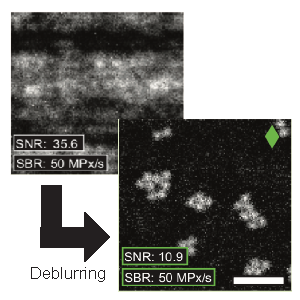
\includegraphics[width=\linewidth]{avatar_highthroughput}
\end{wrapfigure}

In Chapter~\ref{ch:highthroughput}, we introduced the concept of high-throughput imaging, and described conventional methods for obtaining images with a wide field-of-view and high resolution. After discussing the limitations of existing methods, we proposed a novel coded illumination technique where measurements are acquired while the sample is in motion, which is synchronized with multiple illumination pulses during each exposure to introduce a known motion blur. These images, which have higher SNR than images captured at the same speed under strobed illumination, are then computationally deblurred to recover the static object at high speed while maintaining the SNR of much slower acquisition methods. We compare our technique to existing methods, stop-and-stare and strobed illumination, which require a significantly longer acquisition time or produce images with significantly lower SNR, respectively. Using a generalized framework for predicting the reconstruction SNR of measurements acquired using each method, we show, through both theory and experiment, that our coded illumination technique can produce images with up to 10$\times$ the SNR of strobed acquisitions, at significantly faster acquisition rates than images captured under strobed illumination.

\begin{wrapfigure}{R}{12em}
  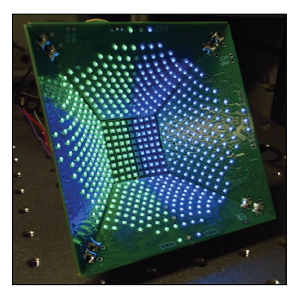
\includegraphics[width=\linewidth]{avatar_fabrication}
\end{wrapfigure}

\noindent of this benefit is not constant across system parameters such as camera readout noise and illumination power. To quantify how our method compares to existing methods, we perform an analysis of the relative performance of our method compared to conventional high-throughput imaging techniques such as strobed illumination or stop-and-stare. For low-light situations such as fluorescence imaging, our method is uniquely suited to provide faster imaging at higher SNR than existing methods.


In Chapter~\ref{ch:fabrication}, we detail the design and fabrication of coded illumination devices for the computational microscopy applications presented in this dissertation. We begin by defining the common design requirements of programmable illumination devices, focusing on programmable LED arrays as our primary application due to their low cost and wide availability. We then describe several design iterations of a programmable LED dome which enables high-angle coded illumination. In the first design iteration, we designed and fabricated a 3D-printed LED dome which was carefully assembled by hand, requiring several months of fabrication. This device was intended to be used with CellScope, a portable microscope platform which uses a smartphone to capture and process images for telemedicine applications. In the second design iteration, we designed and developed a LED quasi-dome which uses 5 printed-circuit boards arranged in a dome-like structure. This device requires significantly less time and effort to assemble and provides RGB illumination across 581 LEDs up to 0.9NA. The ease of manufacturing has enabled the wide distribution of these devices to collaborators around the world. Finally, we describe the Computational CellScope platform in greater detail, which implements coded illumination on a portable platform to perform digital refocusing using light-field methods, quantitative phase imaging, and multi-contrast imaging.


\begin{wrapfigure}{L}{15em}
  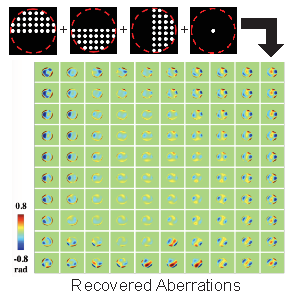
\includegraphics[width=\linewidth]{avatar_selfcal}
\end{wrapfigure}


In Chapter ~\ref{ch:selfcal}, two methods for self-calibration of computational imaging systems are described. Computational imaging methods are uniquely susceptible to mis-calibration since the inferred forward model is often assumed to be ideally calibrated. In reality, the forward model is a function of the optical physics and optical design (which can be inferred), as well as mis-calibration, which cannot be assumed to be negligible in many systems. We first discuss a technique for performing aberration self-calibration using differential phase contrast. Our method employs an alternating-minimization approach to solve for both the complex field of the object as well as the aberrations, which are projected into a Zernike basis. This method is non-convex, but is differentiable, and guaranteed not to diverge so long as an appropriate step size is used. Further, we use a patch-wise solver to solve for aberrations across the field, revealing spatially variant aberration functions. We verify our method by solving for the defocus aberration when introducing a known defocus term. Our method requires only a single coherent measurement, in addition to three DPC measurements for recovering the object's complex field. Next, we presented a method for performing self-calibration of LED positions in both the brightfield and darkfield regions for Fourier ptychography. After performing a brightfield calibration method, we employ a novel gradient-based technique for solving for the homography between printed circuit boards in a quasi-dome device. This technique makes the alternating minimization process much more stable and enables high-NA Fourier ptychography with resolution below 450nm. While a good hardware system alignment is most effective, these self-calibration techniques can mitigate mis-calibration when this is not possible.
\clearpage

\section{Entrepreneurship in Computational Microscopy}
During my time at Berkeley I was fortunate to benefit from the many resources for entrepreneurship on campus. Along with fellow lab member Michael Chen and my advisor Laura Waller, I founded Spectral Coded Illumination, Inc. in early 2017 with the purpose of bridging the gap between the scientific publication of our prototypes and the large-scale distribution of LED dome prototypes. The initial motivation to form this venture came from the early Quasi-dome prototype presented in Chapter~\ref{ch:ch:fabrication}, Section~\ref{sec:sec:fabrication:quasidome}, which brought significant interest from both collaborators and visitors from industry. After quickly distributing our initial production run of 10 Quasi-domes through the Waller Lab, we saw a need in both industry and academia for functional LED dome prototypes and sought to use our knowledge in this area to drive progress in our research field at a larger scale. We began by getting involved on through campus programs, including the NSF I-Corps program, the Citris Foundry, Berkeley Skydeck, and the Bakar Innovation Fellows program, which allowed us to meet other entrepreneurs in the sciences and better understand how to build a successful scientific venture. For the past 2.5 years we have continued to sell LED domes and provide consulting services in areas related to our research for the past two and a half years, selling over 15 LED arrays across the United States and in Europe, to customers in both industry and academia.

I view this experience as a critical component of my education at Berkeley, as it allowed me to view my research with a broader view, and to understand the effort and technical challenges which come with commercializing and scaling up a research proposal. While the direct motivations for forming a corporation can be quite different from academic research, I have found that my underlying motivation for both ventures has been the same: to accelerate the pace of scientific discovery through the development of novel imaging methods and hardware. Having a start-up motivated me to align my research to be more useful for the field at-large, which has been very useful in the later stages of my education.

\section{Proposed Future Work}
As my time at Berkeley comes to a close, there are still many open questions which I find interesting and would like to pursue, given the opportunity. In the future, I hope that myself or someone else will have the time and a motivation to explore a few of the following proposals.

The first, and most general, is the application of a task-based imaging paradigm to the applications discussed in this work. In each of the previous chapters, we have quantified the quality of our reconstructions using system parameters such as signal-to-noise ratio, acquisition throughput (space-bandwidth rate), resolving power and field of view. Rarely is emphasis placed on the quality of these images towards a specific task, such as cell counting, pathogen recognition, or disease diagnosis. Conventionally the field of computational imaging has tended to focus on imaging system performance, but I believe that defining a differentiable performance metric (cost function) which is relevant to the imaging task would be extremely interesting. As a first step, I would propose cell-counting as a metric. Recent work from the machine learning community has proposed optimizing network layers for the counting and classification of cells~\cite{falk2019unet, xue2017cell}. Including programmable hardware elements (such as LED arrays which could introduce different contrast) into the learning pipeline could provide significant improvements in counting accuracy and performance.

A second, more specific future direction, is the application of compressed sensing to solve under-determined motion deblurring problems for slide-scanning and digital pathology applications. Currently, the volume of data required for large-scale imaging (e.g. neuropathology) can make acquisition times and data storage difficult or infeasible. If data acquisition processing requirements were lower, acquisitions could be made much faster, and large-scale imaging analysis could be more readily performed. For a compressed-sensing acquisition to perform well, the aliasing introduced by undersampling should be incoherent with a domain in which the sample is sparse. An acquisition with a random forward operator is one example of such a forward model, because this matrix is incoherent with every other matrix. While it is very difficult to design a truly random forward operator in this problem, we have control over the structure of our forward operator through the illumination sequence as well as the motion pathway. So long as this acquisition introduces incoherent aliasing, we have some hope of reconstructing a sparse object from an under-determined system. To accomplish this, I would propose optimizing the entire pipeline using an unrolled network, which allows us to differentiate with simple parameters such as step size as well as more complicated parameters, such as the sparsifying operator or acquisition strategy. Using large amounts of training data, we could then generate a principled acquisition and reconstruction strategy together which would enhance the capabilities of high-throughput acquisitions well-beyond those presented in this work.

A third future direction is active imaging, or the active determination of acquisition trajectories based on current image data. These trajectories need not span Cartesian space, but could also include LED angle, defocused positions, or other metrics. A key component to these methods being advantageous would be that the sample should be localized, meaning that most of the densely sampled data is unnecessary, and that the learning process should be fast, so that the compute + scan time does not exceed the time to densely scan a sample. An obvious example of this would be multi-well plates, where a microscope may perform a fast scan over many wells which aliases them together, then uses this blurred data to determine which wells are worth imaging more closely at high-resolution for quantification. Such a technique could speed up acquisitions significantly for many applications.

In terms of fabrication of LED devices, I believe that engineering improvements in the power supply of the devices as well as a more careful layout of the high-speed traces (such as serial clock and pulse-width-modulation clock) would enable imaging with shorter exposure times. In addition, a more compact portable microscope device incorporating a PCB-based LED array would be much more robust than the current Computational CellScope device, enabling wider distribution to collaborators around the world.

I have made much of my existing code available under the BSD open-source license at repositories listed in Appendix, Section~\ref{sec:appendix:opensource}. I hope that these examples and this dissertation will inspire others to iterate and advance the field of computational imaging.

\chapter{Appendix} \label{ch:appendix}

\section{Open-Source Code} \label{sec:appendix:opensource}
Open-source availability
\section{High-Throughput System Analysys}  \label{sec:appendix:highthroughput}
\subsection{Derivation of SNR Expression}
\label{sec:snr_derivation}

In this section we derive the expression for the SNR of a recovered image. Considering the additive noise acquisition model, $\y = \A\x + \noise$, 
the recovered image $\widehat \x$ is given by:
\[\widehat \x =  \A^\dagger  \y = \x +  \A^\dagger  \noise\:.\]
In what follows, we assume only that $\noise$ is zero mean with covariance $\sigma_\noise^2 \I$,

Defining the mean of the recovered object $\mu = \mathbb{E}[\widehat \x]$, as well as the covariance $\mat\Sigma = \mathbb{E}[(\widehat \x-\x) (\widehat \x-\x)^\top]$, we calculate the imaging SNR using the root mean squared error (RMSE):
\[SNR = \frac{\frac{1}{m}\sum_{i=1}^m\mu_i}{\sqrt{\frac{1}{m}\mathrm{Tr}(\mat\Sigma)}}\:.\]
Assuming zero-mean noise, the numerator is simply the average object signal $\bar s$.
Expanding the covariance term in the denominator,
\begin{align*}
    \Sigma &= \mathbb{E}[ \A^\dagger  \noise( \A^\dagger  \noise)^\top]
    %\\
    %&= \mathbb{E}[ A^\dagger  \eta\eta ^\top ( A^\dagger)^\top] 
    = \sigma_{ \noise}^2  \A^\dagger ( \A^\dagger)^\top\:,
\end{align*}
where we apply the assumption that the covariance of $\noise$ is $\sigma_\noise^2 \I$. Then,
\[\mathrm{Tr}( \A^\dagger ( \A^\dagger)^\top ) = \sum_{i=1}^m \frac{1}{\sigma_i( \A)^2} = \frac{1}{\sigma_1(\A)^2} \sum_{i=1}^m \frac{\sigma_1(\A)^2}{\sigma_i(\A)^2} \:.\]
Thus we have that
\[SNR = \frac{\bar s}{\frac{1}{\sigma_1(\A)} \sqrt{\frac{1}{m}\sum_{i=1}^m \frac{\sigma_1(\A)}{\sigma_i(\A)}} \cdot\sigma_\eta} := \frac{\sigma_1(\A) \bar s }{ f\sigma_\eta }\:,\]
where $f$ is the general definition of the deconvolution noise factor. This expression is consistent with the definition in~\eqref{eq:DNF} for convolutional operators, where we note that the singular values are given by the power spectrum of the kernel $\h$. Further, we note that in this case $\sigma_1(\A)=\gamma$ since that is the DC component of a non-negative signal.

\subsection{Multi-frame Decomposition}\label{sec:multiframe_app}

We consider the case of a multiframe operator with the same blur kernel $\h$ used in every frame. In this case, the forward operator has the form
\begin{equation*}
\A =  \begin{bmatrix}\W_1 \\ \vdots \\ \W_n \end{bmatrix}\B := \W\B\:.
\end{equation*}
 Following the derivation of SNR from the previous section, we compute $\mathrm{Tr}(\A^\dagger (\A^\dagger)^\top)$. First,
\[\A^\dagger = (\B^\top {\W}^\top{\W} \B)^{-1} \B^\top {\W}^\top =
\B^{-1} ({\W}^\top{\W} )^{-1} {\W}^\top\:,\]
assuming that $\B$ and $\W^\top \W$ are invertible.
Then we have that
\begin{align*}
    \mathrm{Tr}(\A^\dagger &(\A^\dagger)^\top) = \mathrm{Tr}(\B^{-1} ({\W}^\top{\W} )^{-1} {\W}^\top {\W} ({\W}^\top{\W} )^{-\top}
    \B^{-\top}) \\
    &= \mathrm{Tr}(\B^{-1} ({\W}^\top{\W} )^{-1}
    \B^{-1}) = \mathrm{Tr}(({\W}^\top{\W} )^{-1} \B^{-2} )\:.
\end{align*}
We now consider the form of ${\W}^\top{\W} = \sum_{j=1}^n \W_j^\top \W_j$. Each $\W_j^\top \W_j$ is a square diagonal matrix with either a $0$ or $1$ for each diagonal entry, depending on whether the corresponding pixel is included in the window. Thus the sum ${\W}^\top {\W}$ is a diagonal matrix with the $i$th diagonal value given by the number of times pixel $i$ is included in the windows $\{\W_1,...,\W_n\}$, a quantity we denote as $c_i = \sum_{j=1}^n \W_j \e_i$ where $\{\e_i\}$ are the standard basis vectors.
% \begin{align*}
%     \mathrm{Tr}(A^\dagger &(A^\dagger)^\top) = \mathrm{Tr}(B^{-2} \mathrm{diag}(c_1^{-1},...,c_m^{-1}))\:.
% \end{align*}

Before we proceed further, note that for any matrices $\M$ and $\D$ with non-negative entries and $\D$ diagonal,
\[\mathrm{Tr}(\D\M) = \sum_{i} D_{ii} M_{ii}  \leq \max_{i} D_{ii} \cdot \mathrm{Tr}(\M)\:.\]
% Then we have that
% \begin{align*}
% \kappa(A) &= \kappa({W} B) \\&\leq \kappa({W}) \cdot \kappa(B) = \frac{\max_{j}c_j}{\min_{j}c_j} \cdot \frac{\max_i |\tilde h|_i}{\min_i |\tilde h|_i}\:.
% \end{align*}
% Since the condition number is an upper bound on the DNF, this provides a lower bound on SNR for this multiframe case.
We can therefore conclude that
\begin{align*}
    \mathrm{Tr}(\A^\dagger (\A^\dagger)^\top)&\leq \max_{i}\frac{1}{c_i}\cdot \mathrm{Tr}(\B^{-2})
    =
    \frac{1}{\min_{i} c_i}   \cdot \sum_{i=1}^m \frac{1}{|\tilde \h|_i^2}\:.
\end{align*}
Thus we see that the expression for the covariance is decreased by a factor of at least the square root of minimum coverage. This corresponds to the lower bound on the SNR:
\[SNR \geq \sqrt{{\min_{i} c_i}}\cdot \frac{ \gamma\bar s}{ f \sigma_\eta  }\:.\]
Where $f$ is defined as in~\eqref{eq:DNF}.



\subsection{Blur Kernel Optimization} \label{sec:optimization_app}

In this section we discuss the reformulation of
the optimization problem in~\eqref{eq:illum_opt_single} as a smooth objective with convex constraints.
Recall that the optimization problem has the form
\begin{align*}
\min_{\h}&~~ \sqrt{\frac{1}{m} \sum_{i=0}^m \frac{\max_i{|\tilde{\h}|_i^2}}{|\tilde{\h}|_i^2}} \\
  s.t. &~~0 \leq h_i \leq 1 \; \forall \; i, \quad
  \sum_{i} h_i = \gamma \:.
\end{align*}
First, note that by definition $\tilde \h=\F\h$ where $\F$ represents the discrete Fourier transform (DFT) matrix.
Then, we know that $\max_i{|\tilde{\h}|_i^2}$ is the DC component of the signal, which is equal to $\gamma$ and therefore fixed for any feasible $\h$.
Therefore, the blur kernel which maximizes~\eqref{eq:illum_opt_single} is the same as the one that maximizes
\begin{align*}
\label{eq:opt_smooth}
\min_{\h}&~~ \sum_{i=0}^m \frac{1}{(\F_i^\top\h)^2} ~~
  s.t. ~~0 \leq h_i \leq 1, ~
  \sum_{i} h_i = \gamma \:,
\end{align*}
where $\F_i$ represents columns of the DFT matrix.

It is possible to use projected gradient methods because the objective function is smooth nearly everywhere and the constraints are convex. At each iteration, there is a gradient step followed by a projection step.
The gradient step is defined as
\begin{align*}
    \tilde \h^{k+1} = \h^k + \alpha^k \sum_{i=0}^m   \frac{2}{(\F_i^\top \h^k)^{3}} \cdot \F_i\:,
\end{align*}
for potentially changing step size $\alpha^k$.
%\nabla \sum_{i=0}^m \frac{1}{(F_i^\top h)^2} = \sum_{i=0}^m   -2(F_i^\top h)^{-3} \cdot \nabla (F_i^\top h)= 
The projection step is defined as
\begin{align*}
    \h^{k+1} = \Pi_{\mathcal{S}}(\tilde \h_{k+1})\:,
\end{align*}
where $\mathcal{S}$ is the intersection of the box constraint $\{0\leq h_i\leq 1\}$ and the simplex constraint $\{\sum_i h_i = \gamma\}$. Efficent methods for this projection exist~\cite{,gupta2010l1}.

\subsection{Fundamental DNF Limits}\label{sec:dnf_limit}

There are fundamental limits on how SNR can be improved by coded illumination.
We examine a fundamental lower bound on the DNF to demonstrate this.

Recall that
\[f^2 = \max_i |\tilde \h|_i^2\cdot \frac{1}{m} \sum_{i=1}^m \frac{1}{|\tilde \h|_i^2}\:.\]
Then, note that $\frac{1}{m} \sum_{i=1}^m \frac{1}{|\tilde \h|_i^2}$ is the reciprocal of the {harmonic mean} of $\{|\tilde \h|_1^2,...,|\tilde \h|_m^2\}$. Since the harmonic mean is always less than the {arithmetic mean}, we have that
$$ \frac{1}{m} \sum_{i=1}^m \frac{1}{|\tilde \h|_i^2}\geq \frac{1}{\frac{1}{m}\sum_{i=1}^m |\tilde \h|_i^2}\:. $$

Next, we apply Parseval's and have $\frac{1}{m}\sum_{i=1}^m |\tilde \h|_i^2 = \sum_{i=1}^m h_i^2$.
Additionally, $\max_i |\tilde \h|_i$ is the DC component of the signal, which is specified by the constraint $\sum_{i=1}^m h_i = \gamma$.
As a result, $$ f^2 \geq \frac{\gamma^2}{\sum_{i=1}^m h_i^2}\:.$$
Finally, we see that
$$\max_{\h\in[0,1]^m} \sum_{i=1}^m h_i^2~:~ \sum_{i=1}^m h_i=\gamma$$
is achieved for binary $h$ and has the maximum value $\gamma$. Therefore, 
\[f^2 \geq \frac{\gamma^2}{\sum_{i=1}^m h_i^2} \geq \frac{\gamma^2}{\gamma} = \gamma\:.\]
% \begin{lem}
% We have the following relationship between average squared singular value and illumination values, $\frac{1}{m}\sum_{i=1}^m |\tilde h|_i^2 = \sum_{j=1}^d v_j^2$.
% \end{lem}
% \begin{proof}
% First, note that $\tilde h = Fh = F\sum_{j=1}^d v_j \delta_j$. Then the average squared singular values is given by the inner product
% $$\frac{1}{m} \sum_{i=1}^m |\tilde h|_i^2 = \frac{1}{m} (Fh)^H Fh =  \frac{1}{m} \sum_{j=1}^n \sum_{\ell=1}^n v_jv_\ell \delta_j^H F^H F\delta_\ell =  \sum_{j=1}^n  v_j^2 $$
% where the final simplification comes from noting that $F^H F = mI$ (since we use un-normalized DFT matrices, TODO) and $\delta_j^H\delta_\ell = \mathbf{1}\{j=\ell\}$.
% \end{proof}
That is, the DNF grows at a rate of at least $\sqrt{\gamma}$. As a result,  the best achievable SNR (using~\eqref{eq:snr_coded}) is
$$ SNR  \leq \frac{\sqrt{\gamma}\bar{s}_0}{\sqrt{\gamma\bar{s}_0 + \sigma^2_{r}}}
=\sqrt{\bar{s}_0}\sqrt{\frac{\gamma \bar{s}_0 }{\gamma\bar{s}_0 + \sigma^2_{r}}}\:,
$$
This upper bound on SNR increases with ${\gamma}$.
In Methods Section~\ref{sec:illum_opt}, we discuss an exact closed form for $f(\gamma)$ that yields an expression for optimal multiplexing.

However, if $\sigma_r$ is much smaller than the total captured signal, i.e. $\sigma_r \ll \gamma \bar{s}_0 $, the SNR will not increase with $\gamma$, and in fact its maximum value,
$$SNR \leq \sqrt{\bar{s}_0}$$
is achieved by strobed illumination (i.e. $\gamma=1$). In other words, when signal is large compared with readout noise, strobed will be optimal, regardless of the illumination optimization method.


\subsection{Derivation of Illumination Throughput}\label{sec:app_throughput}

\subsubsection{Stop-and-Stare}
In the stop-and-stare acquisition strategy, the sample is illuminated for the full dwell time ($t_{sns}$), which is set by motion stage parameters such as maximum velocity, acceleration, and the necessary stage settle time ($v_{stage}$, $a_{stage}$, and $t_{settle}$ respectively), as well as camera readout ($t_{readout}$). These parameters are related to frame rate $r_{frame}$ by the following relationship:
\begin{equation*}
t_{sns} = \frac{1}{r_{frame}} - \max (t_{readout}, 2t_{accel} + t_{move})
\end{equation*}

Note that this equation assumes perfect hardware synchronization and instantaneous acceleration ($\frac{\partial a}{\partial t} = \infty$). The variables $t_{accel}$ and $t_{move}$ are defined as:

\begin{equation*}
t_{accel} = \frac{v_{stage}}{a_{stage}}
\end{equation*}

\begin{equation*}
t_{move} = \frac{d_{frame} - 0.5 * a_{stage} * t_{accel}^2}{v_{stage}}
\end{equation*}

Here the expression $d_{frame} = FOV * (1-O)$ is the distance between frames, which is determined by the field-of-view of a single frame ($FOV$) and inter-frame overlap fraction $O$.

Combining terms, we arrive at an expression for $t_{sns}$:
\begin{equation*}
t_{sns} = \frac{1}{r_{frame}} - \max (t_{readout}, 2\frac{v_{stage}}{a_{stage}} - \frac{d_{frame} - 0.5 * a_{stage} * t_{accel}^2}{v_{stage}})
\end{equation*}

When camera readout time $t_{readout}$ is short, $t_{sns}$ can be simplified to:

\begin{equation*}
t_{sns} = \frac{1}{r_{frame}} - 2\frac{v_{stage}}{a_{stage}} - \frac{d_{frame} - 0.5 * \frac{v_{stage}^2}{a_{stage}}}{v_{stage}}
\end{equation*}

\subsubsection{Strobed Illumination}

The maximum pulse duration for strobed illumination is related to the time required to move a distance of one effective pixel size $\frac{\Delta}{M}$ at a velocity $v_{stage}$:
\begin{equation*}
t_{strobe} = \frac{\frac{\Delta}{M}}{v_{stage}}
\end{equation*}

The stage velocity $v_{stage}$ may be bounded by the motion stage hardware ($v_{max}$) or by the field of view of the microscope ($FOV$):

\begin{equation*}
v_{stage} = \min (v_{max}, r_{frame}FOV)
\end{equation*}

\subsubsection{Coded Illumination}
The calculation of $t_{coded}$ for coded illumination is synonymous to the strobed illumination case, weighted by the multiplexing coefficient used to generate the illumination sequence ($\gamma$), and using the $v_{stage}$ calculation from the strobed subsection:
\begin{equation*}
t_{coded} = \frac{\frac{\gamma \Delta}{M}}{v_{stage}}
\end{equation*}

\subsection{System Parameters}\label{sec:sys_param}
    \begin{center}
    \begin{tabular}{ | c | c |}
    \hline
    \textbf{Parameter} & \textbf{Value} \\ 
    \hline
    Maximum Motion Stage Velocity & $40\frac{m}{s}$ \\ 
    \hline
    Motion Stage Acceleration & $400 \frac{m}{s^2}$\\
    \hline
    Motion Stage Settle Time & $0.1s$\\
    \hline
    Objective Mag / NA& $10\times / 0.25NA$\\
    \hline
    Frame Overlap & $20\%$ \\
    \hline
    Illumination Power & $600$ \\
    \hline
    Camera Readout Time & 26ms\\
    \hline
    Camera Readout Noise & 3.7 $e^-$ \\
    \hline
    Camera Quantum Efficiency & $60\%$ \\
    \hline
    Camera Pixel Size & $6.5\mu m$\\
    \hline
    Fluorophore Quantum Yield& $79\%$ lux\\
    \hline
    Illumination repetition Rate & $250 kHz$\\
     \hline
    \end{tabular}
\end{center}


\bibstyle{osajnl}
\bibliography{references}

\end{document}
